\documentclass[a4paper, 10pt] {report}
% general packages
\usepackage{html}
\usepackage{tabularx}
\usepackage{multirow}
\usepackage{graphicx}
\usepackage{hyperref}
\usepackage{color}
\usepackage{listings}
\definecolor{AliceBlue}{rgb}{0.94,0.97,1.00}
\definecolor{AntiqueWhite1}{rgb}{1.00,0.94,0.86}
\definecolor{AntiqueWhite2}{rgb}{0.93,0.87,0.80}
\definecolor{AntiqueWhite3}{rgb}{0.80,0.75,0.69}
\definecolor{AntiqueWhite4}{rgb}{0.55,0.51,0.47}
\definecolor{AntiqueWhite}{rgb}{0.98,0.92,0.84}
\definecolor{BlanchedAlmond}{rgb}{1.00,0.92,0.80}
\definecolor{BlueViolet}{rgb}{0.54,0.17,0.89}
\definecolor{CadetBlue1}{rgb}{0.60,0.96,1.00}
\definecolor{CadetBlue2}{rgb}{0.56,0.90,0.93}
\definecolor{CadetBlue3}{rgb}{0.48,0.77,0.80}
\definecolor{CadetBlue4}{rgb}{0.33,0.53,0.55}
\definecolor{CadetBlue}{rgb}{0.37,0.62,0.63}
\definecolor{CornflowerBlue}{rgb}{0.39,0.58,0.93}
\definecolor{DarkBlue}{rgb}{0.00,0.00,0.55}
\definecolor{DarkCyan}{rgb}{0.00,0.55,0.55}
\definecolor{DarkGoldenrod1}{rgb}{1.00,0.73,0.06}
\definecolor{DarkGoldenrod2}{rgb}{0.93,0.68,0.05}
\definecolor{DarkGoldenrod3}{rgb}{0.80,0.58,0.05}
\definecolor{DarkGoldenrod4}{rgb}{0.55,0.40,0.03}
\definecolor{DarkGoldenrod}{rgb}{0.72,0.53,0.04}
\definecolor{DarkGray}{rgb}{0.66,0.66,0.66}
\definecolor{DarkGreen}{rgb}{0.00,0.39,0.00}
\definecolor{DarkGrey}{rgb}{0.66,0.66,0.66}
\definecolor{DarkKhaki}{rgb}{0.74,0.72,0.42}
\definecolor{DarkMagenta}{rgb}{0.55,0.00,0.55}
\definecolor{DarkOliveGreen1}{rgb}{0.79,1.00,0.44}
\definecolor{DarkOliveGreen2}{rgb}{0.74,0.93,0.41}
\definecolor{DarkOliveGreen3}{rgb}{0.64,0.80,0.35}
\definecolor{DarkOliveGreen4}{rgb}{0.43,0.55,0.24}
\definecolor{DarkOliveGreen}{rgb}{0.33,0.42,0.18}
\definecolor{DarkOrange1}{rgb}{1.00,0.50,0.00}
\definecolor{DarkOrange2}{rgb}{0.93,0.46,0.00}
\definecolor{DarkOrange3}{rgb}{0.80,0.40,0.00}
\definecolor{DarkOrange4}{rgb}{0.55,0.27,0.00}
\definecolor{DarkOrange}{rgb}{1.00,0.55,0.00}
\definecolor{DarkOrchid1}{rgb}{0.75,0.24,1.00}
\definecolor{DarkOrchid2}{rgb}{0.70,0.23,0.93}
\definecolor{DarkOrchid3}{rgb}{0.60,0.20,0.80}
\definecolor{DarkOrchid4}{rgb}{0.41,0.13,0.55}
\definecolor{DarkOrchid}{rgb}{0.60,0.20,0.80}
\definecolor{DarkRed}{rgb}{0.55,0.00,0.00}
\definecolor{DarkSalmon}{rgb}{0.91,0.59,0.48}
\definecolor{DarkSeaGreen1}{rgb}{0.76,1.00,0.76}
\definecolor{DarkSeaGreen2}{rgb}{0.71,0.93,0.71}
\definecolor{DarkSeaGreen3}{rgb}{0.61,0.80,0.61}
\definecolor{DarkSeaGreen4}{rgb}{0.41,0.55,0.41}
\definecolor{DarkSeaGreen}{rgb}{0.56,0.74,0.56}
\definecolor{DarkSlateBlue}{rgb}{0.28,0.24,0.55}
\definecolor{DarkSlateGray1}{rgb}{0.59,1.00,1.00}
\definecolor{DarkSlateGray2}{rgb}{0.55,0.93,0.93}
\definecolor{DarkSlateGray3}{rgb}{0.47,0.80,0.80}
\definecolor{DarkSlateGray4}{rgb}{0.32,0.55,0.55}
\definecolor{DarkSlateGray}{rgb}{0.18,0.31,0.31}
\definecolor{DarkSlateGrey}{rgb}{0.18,0.31,0.31}
\definecolor{DarkTurquoise}{rgb}{0.00,0.81,0.82}
\definecolor{DarkViolet}{rgb}{0.58,0.00,0.83}
\definecolor{DeepPink1}{rgb}{1.00,0.08,0.58}
\definecolor{DeepPink2}{rgb}{0.93,0.07,0.54}
\definecolor{DeepPink3}{rgb}{0.80,0.06,0.46}
\definecolor{DeepPink4}{rgb}{0.55,0.04,0.31}
\definecolor{DeepPink}{rgb}{1.00,0.08,0.58}
\definecolor{DeepSkyBlue1}{rgb}{0.00,0.75,1.00}
\definecolor{DeepSkyBlue2}{rgb}{0.00,0.70,0.93}
\definecolor{DeepSkyBlue3}{rgb}{0.00,0.60,0.80}
\definecolor{DeepSkyBlue4}{rgb}{0.00,0.41,0.55}
\definecolor{DeepSkyBlue}{rgb}{0.00,0.75,1.00}
\definecolor{DimGray}{rgb}{0.41,0.41,0.41}
\definecolor{DimGrey}{rgb}{0.41,0.41,0.41}
\definecolor{DodgerBlue1}{rgb}{0.12,0.56,1.00}
\definecolor{DodgerBlue2}{rgb}{0.11,0.53,0.93}
\definecolor{DodgerBlue3}{rgb}{0.09,0.45,0.80}
\definecolor{DodgerBlue4}{rgb}{0.06,0.31,0.55}
\definecolor{DodgerBlue}{rgb}{0.12,0.56,1.00}
\definecolor{FloralWhite}{rgb}{1.00,0.98,0.94}
\definecolor{ForestGreen}{rgb}{0.13,0.55,0.13}
\definecolor{GhostWhite}{rgb}{0.97,0.97,1.00}
\definecolor{GreenYellow}{rgb}{0.68,1.00,0.18}
\definecolor{HotPink1}{rgb}{1.00,0.43,0.71}
\definecolor{HotPink2}{rgb}{0.93,0.42,0.65}
\definecolor{HotPink3}{rgb}{0.80,0.38,0.56}
\definecolor{HotPink4}{rgb}{0.55,0.23,0.38}
\definecolor{HotPink}{rgb}{1.00,0.41,0.71}
\definecolor{IndianRed1}{rgb}{1.00,0.42,0.42}
\definecolor{IndianRed2}{rgb}{0.93,0.39,0.39}
\definecolor{IndianRed3}{rgb}{0.80,0.33,0.33}
\definecolor{IndianRed4}{rgb}{0.55,0.23,0.23}
\definecolor{IndianRed}{rgb}{0.80,0.36,0.36}
\definecolor{LavenderBlush1}{rgb}{1.00,0.94,0.96}
\definecolor{LavenderBlush2}{rgb}{0.93,0.88,0.90}
\definecolor{LavenderBlush3}{rgb}{0.80,0.76,0.77}
\definecolor{LavenderBlush4}{rgb}{0.55,0.51,0.53}
\definecolor{LavenderBlush}{rgb}{1.00,0.94,0.96}
\definecolor{LawnGreen}{rgb}{0.49,0.99,0.00}
\definecolor{LemonChiffon1}{rgb}{1.00,0.98,0.80}
\definecolor{LemonChiffon2}{rgb}{0.93,0.91,0.75}
\definecolor{LemonChiffon3}{rgb}{0.80,0.79,0.65}
\definecolor{LemonChiffon4}{rgb}{0.55,0.54,0.44}
\definecolor{LemonChiffon}{rgb}{1.00,0.98,0.80}
\definecolor{LightBlue1}{rgb}{0.75,0.94,1.00}
\definecolor{LightBlue2}{rgb}{0.70,0.87,0.93}
\definecolor{LightBlue3}{rgb}{0.60,0.75,0.80}
\definecolor{LightBlue4}{rgb}{0.41,0.51,0.55}
\definecolor{LightBlue}{rgb}{0.68,0.85,0.90}
\definecolor{LightCoral}{rgb}{0.94,0.50,0.50}
\definecolor{LightCyan1}{rgb}{0.88,1.00,1.00}
\definecolor{LightCyan2}{rgb}{0.82,0.93,0.93}
\definecolor{LightCyan3}{rgb}{0.71,0.80,0.80}
\definecolor{LightCyan4}{rgb}{0.48,0.55,0.55}
\definecolor{LightCyan}{rgb}{0.88,1.00,1.00}
\definecolor{LightGoldenrod1}{rgb}{1.00,0.93,0.55}
\definecolor{LightGoldenrod2}{rgb}{0.93,0.86,0.51}
\definecolor{LightGoldenrod3}{rgb}{0.80,0.75,0.44}
\definecolor{LightGoldenrod4}{rgb}{0.55,0.51,0.30}
\definecolor{LightGoldenrodYellow}{rgb}{0.98,0.98,0.82}
\definecolor{LightGoldenrod}{rgb}{0.93,0.87,0.51}
\definecolor{LightGray}{rgb}{0.83,0.83,0.83}
\definecolor{LightGreen}{rgb}{0.56,0.93,0.56}
\definecolor{LightGrey}{rgb}{0.83,0.83,0.83}
\definecolor{LightPink1}{rgb}{1.00,0.68,0.73}
\definecolor{LightPink2}{rgb}{0.93,0.64,0.68}
\definecolor{LightPink3}{rgb}{0.80,0.55,0.58}
\definecolor{LightPink4}{rgb}{0.55,0.37,0.40}
\definecolor{LightPink}{rgb}{1.00,0.71,0.76}
\definecolor{LightSalmon1}{rgb}{1.00,0.63,0.48}
\definecolor{LightSalmon2}{rgb}{0.93,0.58,0.45}
\definecolor{LightSalmon3}{rgb}{0.80,0.51,0.38}
\definecolor{LightSalmon4}{rgb}{0.55,0.34,0.26}
\definecolor{LightSalmon}{rgb}{1.00,0.63,0.48}
\definecolor{LightSeaGreen}{rgb}{0.13,0.70,0.67}
\definecolor{LightSkyBlue1}{rgb}{0.69,0.89,1.00}
\definecolor{LightSkyBlue2}{rgb}{0.64,0.83,0.93}
\definecolor{LightSkyBlue3}{rgb}{0.55,0.71,0.80}
\definecolor{LightSkyBlue4}{rgb}{0.38,0.48,0.55}
\definecolor{LightSkyBlue}{rgb}{0.53,0.81,0.98}
\definecolor{LightSlateBlue}{rgb}{0.52,0.44,1.00}
\definecolor{LightSlateGray}{rgb}{0.47,0.53,0.60}
\definecolor{LightSlateGrey}{rgb}{0.47,0.53,0.60}
\definecolor{LightSteelBlue1}{rgb}{0.79,0.88,1.00}
\definecolor{LightSteelBlue2}{rgb}{0.74,0.82,0.93}
\definecolor{LightSteelBlue3}{rgb}{0.64,0.71,0.80}
\definecolor{LightSteelBlue4}{rgb}{0.43,0.48,0.55}
\definecolor{LightSteelBlue}{rgb}{0.69,0.77,0.87}
\definecolor{LightYellow1}{rgb}{1.00,1.00,0.88}
\definecolor{LightYellow2}{rgb}{0.93,0.93,0.82}
\definecolor{LightYellow3}{rgb}{0.80,0.80,0.71}
\definecolor{LightYellow4}{rgb}{0.55,0.55,0.48}
\definecolor{LightYellow}{rgb}{1.00,1.00,0.88}
\definecolor{LimeGreen}{rgb}{0.20,0.80,0.20}
\definecolor{MediumAquamarine}{rgb}{0.40,0.80,0.67}
\definecolor{MediumBlue}{rgb}{0.00,0.00,0.80}
\definecolor{MediumOrchid1}{rgb}{0.88,0.40,1.00}
\definecolor{MediumOrchid2}{rgb}{0.82,0.37,0.93}
\definecolor{MediumOrchid3}{rgb}{0.71,0.32,0.80}
\definecolor{MediumOrchid4}{rgb}{0.48,0.22,0.55}
\definecolor{MediumOrchid}{rgb}{0.73,0.33,0.83}
\definecolor{MediumPurple1}{rgb}{0.67,0.51,1.00}
\definecolor{MediumPurple2}{rgb}{0.62,0.47,0.93}
\definecolor{MediumPurple3}{rgb}{0.54,0.41,0.80}
\definecolor{MediumPurple4}{rgb}{0.36,0.28,0.55}
\definecolor{MediumPurple}{rgb}{0.58,0.44,0.86}
\definecolor{MediumSeaGreen}{rgb}{0.24,0.70,0.44}
\definecolor{MediumSlateBlue}{rgb}{0.48,0.41,0.93}
\definecolor{MediumSpringGreen}{rgb}{0.00,0.98,0.60}
\definecolor{MediumTurquoise}{rgb}{0.28,0.82,0.80}
\definecolor{MediumVioletRed}{rgb}{0.78,0.08,0.52}
\definecolor{MidnightBlue}{rgb}{0.10,0.10,0.44}
\definecolor{MintCream}{rgb}{0.96,1.00,0.98}
\definecolor{MistyRose1}{rgb}{1.00,0.89,0.88}
\definecolor{MistyRose2}{rgb}{0.93,0.84,0.82}
\definecolor{MistyRose3}{rgb}{0.80,0.72,0.71}
\definecolor{MistyRose4}{rgb}{0.55,0.49,0.48}
\definecolor{MistyRose}{rgb}{1.00,0.89,0.88}
\definecolor{NavajoWhite1}{rgb}{1.00,0.87,0.68}
\definecolor{NavajoWhite2}{rgb}{0.93,0.81,0.63}
\definecolor{NavajoWhite3}{rgb}{0.80,0.70,0.55}
\definecolor{NavajoWhite4}{rgb}{0.55,0.47,0.37}
\definecolor{NavajoWhite}{rgb}{1.00,0.87,0.68}
\definecolor{NavyBlue}{rgb}{0.00,0.00,0.50}
\definecolor{OldLace}{rgb}{0.99,0.96,0.90}
\definecolor{OliveDrab1}{rgb}{0.75,1.00,0.24}
\definecolor{OliveDrab2}{rgb}{0.70,0.93,0.23}
\definecolor{OliveDrab3}{rgb}{0.60,0.80,0.20}
\definecolor{OliveDrab4}{rgb}{0.41,0.55,0.13}
\definecolor{OliveDrab}{rgb}{0.42,0.56,0.14}
\definecolor{OrangeRed1}{rgb}{1.00,0.27,0.00}
\definecolor{OrangeRed2}{rgb}{0.93,0.25,0.00}
\definecolor{OrangeRed3}{rgb}{0.80,0.22,0.00}
\definecolor{OrangeRed4}{rgb}{0.55,0.15,0.00}
\definecolor{OrangeRed}{rgb}{1.00,0.27,0.00}
\definecolor{PaleGoldenrod}{rgb}{0.93,0.91,0.67}
\definecolor{PaleGreen1}{rgb}{0.60,1.00,0.60}
\definecolor{PaleGreen2}{rgb}{0.56,0.93,0.56}
\definecolor{PaleGreen3}{rgb}{0.49,0.80,0.49}
\definecolor{PaleGreen4}{rgb}{0.33,0.55,0.33}
\definecolor{PaleGreen}{rgb}{0.60,0.98,0.60}
\definecolor{PaleTurquoise1}{rgb}{0.73,1.00,1.00}
\definecolor{PaleTurquoise2}{rgb}{0.68,0.93,0.93}
\definecolor{PaleTurquoise3}{rgb}{0.59,0.80,0.80}
\definecolor{PaleTurquoise4}{rgb}{0.40,0.55,0.55}
\definecolor{PaleTurquoise}{rgb}{0.69,0.93,0.93}
\definecolor{PaleVioletRed1}{rgb}{1.00,0.51,0.67}
\definecolor{PaleVioletRed2}{rgb}{0.93,0.47,0.62}
\definecolor{PaleVioletRed3}{rgb}{0.80,0.41,0.54}
\definecolor{PaleVioletRed4}{rgb}{0.55,0.28,0.36}
\definecolor{PaleVioletRed}{rgb}{0.86,0.44,0.58}
\definecolor{PapayaWhip}{rgb}{1.00,0.94,0.84}
\definecolor{PeachPuff1}{rgb}{1.00,0.85,0.73}
\definecolor{PeachPuff2}{rgb}{0.93,0.80,0.68}
\definecolor{PeachPuff3}{rgb}{0.80,0.69,0.58}
\definecolor{PeachPuff4}{rgb}{0.55,0.47,0.40}
\definecolor{PeachPuff}{rgb}{1.00,0.85,0.73}
\definecolor{PowderBlue}{rgb}{0.69,0.88,0.90}
\definecolor{RosyBrown1}{rgb}{1.00,0.76,0.76}
\definecolor{RosyBrown2}{rgb}{0.93,0.71,0.71}
\definecolor{RosyBrown3}{rgb}{0.80,0.61,0.61}
\definecolor{RosyBrown4}{rgb}{0.55,0.41,0.41}
\definecolor{RosyBrown}{rgb}{0.74,0.56,0.56}
\definecolor{RoyalBlue1}{rgb}{0.28,0.46,1.00}
\definecolor{RoyalBlue2}{rgb}{0.26,0.43,0.93}
\definecolor{RoyalBlue3}{rgb}{0.23,0.37,0.80}
\definecolor{RoyalBlue4}{rgb}{0.15,0.25,0.55}
\definecolor{RoyalBlue}{rgb}{0.25,0.41,0.88}
\definecolor{SaddleBrown}{rgb}{0.55,0.27,0.07}
\definecolor{SandyBrown}{rgb}{0.96,0.64,0.38}
\definecolor{SeaGreen1}{rgb}{0.33,1.00,0.62}
\definecolor{SeaGreen2}{rgb}{0.31,0.93,0.58}
\definecolor{SeaGreen3}{rgb}{0.26,0.80,0.50}
\definecolor{SeaGreen4}{rgb}{0.18,0.55,0.34}
\definecolor{SeaGreen}{rgb}{0.18,0.55,0.34}
\definecolor{SkyBlue1}{rgb}{0.53,0.81,1.00}
\definecolor{SkyBlue2}{rgb}{0.49,0.75,0.93}
\definecolor{SkyBlue3}{rgb}{0.42,0.65,0.80}
\definecolor{SkyBlue4}{rgb}{0.29,0.44,0.55}
\definecolor{SkyBlue}{rgb}{0.53,0.81,0.92}
\definecolor{SlateBlue1}{rgb}{0.51,0.44,1.00}
\definecolor{SlateBlue2}{rgb}{0.48,0.40,0.93}
\definecolor{SlateBlue3}{rgb}{0.41,0.35,0.80}
\definecolor{SlateBlue4}{rgb}{0.28,0.24,0.55}
\definecolor{SlateBlue}{rgb}{0.42,0.35,0.80}
\definecolor{SlateGray1}{rgb}{0.78,0.89,1.00}
\definecolor{SlateGray2}{rgb}{0.73,0.83,0.93}
\definecolor{SlateGray3}{rgb}{0.62,0.71,0.80}
\definecolor{SlateGray4}{rgb}{0.42,0.48,0.55}
\definecolor{SlateGray}{rgb}{0.44,0.50,0.56}
\definecolor{SlateGrey}{rgb}{0.44,0.50,0.56}
\definecolor{SpringGreen1}{rgb}{0.00,1.00,0.50}
\definecolor{SpringGreen2}{rgb}{0.00,0.93,0.46}
\definecolor{SpringGreen3}{rgb}{0.00,0.80,0.40}
\definecolor{SpringGreen4}{rgb}{0.00,0.55,0.27}
\definecolor{SpringGreen}{rgb}{0.00,1.00,0.50}
\definecolor{SteelBlue1}{rgb}{0.39,0.72,1.00}
\definecolor{SteelBlue2}{rgb}{0.36,0.67,0.93}
\definecolor{SteelBlue3}{rgb}{0.31,0.58,0.80}
\definecolor{SteelBlue4}{rgb}{0.21,0.39,0.55}
\definecolor{SteelBlue}{rgb}{0.27,0.51,0.71}
\definecolor{VioletRed1}{rgb}{1.00,0.24,0.59}
\definecolor{VioletRed2}{rgb}{0.93,0.23,0.55}
\definecolor{VioletRed3}{rgb}{0.80,0.20,0.47}
\definecolor{VioletRed4}{rgb}{0.55,0.13,0.32}
\definecolor{VioletRed}{rgb}{0.82,0.13,0.56}
\definecolor{WhiteSmoke}{rgb}{0.96,0.96,0.96}
\definecolor{YellowGreen}{rgb}{0.60,0.80,0.20}
\definecolor{aliceblue}{rgb}{0.94,0.97,1.00}
\definecolor{antiquewhite}{rgb}{0.98,0.92,0.84}
\definecolor{aquamarine1}{rgb}{0.50,1.00,0.83}
\definecolor{aquamarine2}{rgb}{0.46,0.93,0.78}
\definecolor{aquamarine3}{rgb}{0.40,0.80,0.67}
\definecolor{aquamarine4}{rgb}{0.27,0.55,0.45}
\definecolor{aquamarine}{rgb}{0.50,1.00,0.83}
\definecolor{azure1}{rgb}{0.94,1.00,1.00}
\definecolor{azure2}{rgb}{0.88,0.93,0.93}
\definecolor{azure3}{rgb}{0.76,0.80,0.80}
\definecolor{azure4}{rgb}{0.51,0.55,0.55}
\definecolor{azure}{rgb}{0.94,1.00,1.00}
\definecolor{beige}{rgb}{0.96,0.96,0.86}
\definecolor{bisque1}{rgb}{1.00,0.89,0.77}
\definecolor{bisque2}{rgb}{0.93,0.84,0.72}
\definecolor{bisque3}{rgb}{0.80,0.72,0.62}
\definecolor{bisque4}{rgb}{0.55,0.49,0.42}
\definecolor{bisque}{rgb}{1.00,0.89,0.77}
\definecolor{black}{rgb}{0.00,0.00,0.00}
\definecolor{blanchedalmond}{rgb}{1.00,0.92,0.80}
\definecolor{blue1}{rgb}{0.00,0.00,1.00}
\definecolor{blue2}{rgb}{0.00,0.00,0.93}
\definecolor{blue3}{rgb}{0.00,0.00,0.80}
\definecolor{blue4}{rgb}{0.00,0.00,0.55}
\definecolor{blueviolet}{rgb}{0.54,0.17,0.89}
\definecolor{blue}{rgb}{0.00,0.00,1.00}
\definecolor{brown1}{rgb}{1.00,0.25,0.25}
\definecolor{brown2}{rgb}{0.93,0.23,0.23}
\definecolor{brown3}{rgb}{0.80,0.20,0.20}
\definecolor{brown4}{rgb}{0.55,0.14,0.14}
\definecolor{brown}{rgb}{0.65,0.16,0.16}
\definecolor{burlywood1}{rgb}{1.00,0.83,0.61}
\definecolor{burlywood2}{rgb}{0.93,0.77,0.57}
\definecolor{burlywood3}{rgb}{0.80,0.67,0.49}
\definecolor{burlywood4}{rgb}{0.55,0.45,0.33}
\definecolor{burlywood}{rgb}{0.87,0.72,0.53}
\definecolor{cadetblue}{rgb}{0.37,0.62,0.63}
\definecolor{chartreuse1}{rgb}{0.50,1.00,0.00}
\definecolor{chartreuse2}{rgb}{0.46,0.93,0.00}
\definecolor{chartreuse3}{rgb}{0.40,0.80,0.00}
\definecolor{chartreuse4}{rgb}{0.27,0.55,0.00}
\definecolor{chartreuse}{rgb}{0.50,1.00,0.00}
\definecolor{chocolate1}{rgb}{1.00,0.50,0.14}
\definecolor{chocolate2}{rgb}{0.93,0.46,0.13}
\definecolor{chocolate3}{rgb}{0.80,0.40,0.11}
\definecolor{chocolate4}{rgb}{0.55,0.27,0.07}
\definecolor{chocolate}{rgb}{0.82,0.41,0.12}
\definecolor{coral1}{rgb}{1.00,0.45,0.34}
\definecolor{coral2}{rgb}{0.93,0.42,0.31}
\definecolor{coral3}{rgb}{0.80,0.36,0.27}
\definecolor{coral4}{rgb}{0.55,0.24,0.18}
\definecolor{coral}{rgb}{1.00,0.50,0.31}
\definecolor{cornflowerblue}{rgb}{0.39,0.58,0.93}
\definecolor{cornsilk1}{rgb}{1.00,0.97,0.86}
\definecolor{cornsilk2}{rgb}{0.93,0.91,0.80}
\definecolor{cornsilk3}{rgb}{0.80,0.78,0.69}
\definecolor{cornsilk4}{rgb}{0.55,0.53,0.47}
\definecolor{cornsilk}{rgb}{1.00,0.97,0.86}
\definecolor{cyan1}{rgb}{0.00,1.00,1.00}
\definecolor{cyan2}{rgb}{0.00,0.93,0.93}
\definecolor{cyan3}{rgb}{0.00,0.80,0.80}
\definecolor{cyan4}{rgb}{0.00,0.55,0.55}
\definecolor{cyan}{rgb}{0.00,1.00,1.00}
\definecolor{darkblue}{rgb}{0.00,0.00,0.55}
\definecolor{darkcyan}{rgb}{0.00,0.55,0.55}
\definecolor{darkgoldenrod}{rgb}{0.72,0.53,0.04}
\definecolor{darkgray}{rgb}{0.66,0.66,0.66}
\definecolor{darkgreen}{rgb}{0.00,0.39,0.00}
\definecolor{darkgrey}{rgb}{0.66,0.66,0.66}
\definecolor{darkkhaki}{rgb}{0.74,0.72,0.42}
\definecolor{darkmagenta}{rgb}{0.55,0.00,0.55}
\definecolor{darkolive}{rgb}{0.33,0.42,0.18}
\definecolor{darkorange}{rgb}{1.00,0.55,0.00}
\definecolor{darkorchid}{rgb}{0.60,0.20,0.80}
\definecolor{darkred}{rgb}{0.55,0.00,0.00}
\definecolor{darksalmon}{rgb}{0.91,0.59,0.48}
\definecolor{darksea}{rgb}{0.56,0.74,0.56}
\definecolor{darkslate}{rgb}{0.18,0.31,0.31}
\definecolor{darkslate}{rgb}{0.18,0.31,0.31}
\definecolor{darkslate}{rgb}{0.28,0.24,0.55}
\definecolor{darkturquoise}{rgb}{0.00,0.81,0.82}
\definecolor{darkviolet}{rgb}{0.58,0.00,0.83}
\definecolor{deeppink}{rgb}{1.00,0.08,0.58}
\definecolor{deepsky}{rgb}{0.00,0.75,1.00}
\definecolor{dimgray}{rgb}{0.41,0.41,0.41}
\definecolor{dimgrey}{rgb}{0.41,0.41,0.41}
\definecolor{dodgerblue}{rgb}{0.12,0.56,1.00}
\definecolor{firebrick1}{rgb}{1.00,0.19,0.19}
\definecolor{firebrick2}{rgb}{0.93,0.17,0.17}
\definecolor{firebrick3}{rgb}{0.80,0.15,0.15}
\definecolor{firebrick4}{rgb}{0.55,0.10,0.10}
\definecolor{firebrick}{rgb}{0.70,0.13,0.13}
\definecolor{floralwhite}{rgb}{1.00,0.98,0.94}
\definecolor{forestgreen}{rgb}{0.13,0.55,0.13}
\definecolor{gainsboro}{rgb}{0.86,0.86,0.86}
\definecolor{ghostwhite}{rgb}{0.97,0.97,1.00}
\definecolor{gold1}{rgb}{1.00,0.84,0.00}
\definecolor{gold2}{rgb}{0.93,0.79,0.00}
\definecolor{gold3}{rgb}{0.80,0.68,0.00}
\definecolor{gold4}{rgb}{0.55,0.46,0.00}
\definecolor{goldenrod1}{rgb}{1.00,0.76,0.15}
\definecolor{goldenrod2}{rgb}{0.93,0.71,0.13}
\definecolor{goldenrod3}{rgb}{0.80,0.61,0.11}
\definecolor{goldenrod4}{rgb}{0.55,0.41,0.08}
\definecolor{goldenrod}{rgb}{0.85,0.65,0.13}
\definecolor{gold}{rgb}{1.00,0.84,0.00}
\definecolor{gray0}{rgb}{0.00,0.00,0.00}
\definecolor{gray100}{rgb}{1.00,1.00,1.00}
\definecolor{gray10}{rgb}{0.10,0.10,0.10}
\definecolor{gray11}{rgb}{0.11,0.11,0.11}
\definecolor{gray12}{rgb}{0.12,0.12,0.12}
\definecolor{gray13}{rgb}{0.13,0.13,0.13}
\definecolor{gray14}{rgb}{0.14,0.14,0.14}
\definecolor{gray15}{rgb}{0.15,0.15,0.15}
\definecolor{gray16}{rgb}{0.16,0.16,0.16}
\definecolor{gray17}{rgb}{0.17,0.17,0.17}
\definecolor{gray18}{rgb}{0.18,0.18,0.18}
\definecolor{gray19}{rgb}{0.19,0.19,0.19}
\definecolor{gray1}{rgb}{0.01,0.01,0.01}
\definecolor{gray20}{rgb}{0.20,0.20,0.20}
\definecolor{gray21}{rgb}{0.21,0.21,0.21}
\definecolor{gray22}{rgb}{0.22,0.22,0.22}
\definecolor{gray23}{rgb}{0.23,0.23,0.23}
\definecolor{gray24}{rgb}{0.24,0.24,0.24}
\definecolor{gray25}{rgb}{0.25,0.25,0.25}
\definecolor{gray26}{rgb}{0.26,0.26,0.26}
\definecolor{gray27}{rgb}{0.27,0.27,0.27}
\definecolor{gray28}{rgb}{0.28,0.28,0.28}
\definecolor{gray29}{rgb}{0.29,0.29,0.29}
\definecolor{gray2}{rgb}{0.02,0.02,0.02}
\definecolor{gray30}{rgb}{0.30,0.30,0.30}
\definecolor{gray31}{rgb}{0.31,0.31,0.31}
\definecolor{gray32}{rgb}{0.32,0.32,0.32}
\definecolor{gray33}{rgb}{0.33,0.33,0.33}
\definecolor{gray34}{rgb}{0.34,0.34,0.34}
\definecolor{gray35}{rgb}{0.35,0.35,0.35}
\definecolor{gray36}{rgb}{0.36,0.36,0.36}
\definecolor{gray37}{rgb}{0.37,0.37,0.37}
\definecolor{gray38}{rgb}{0.38,0.38,0.38}
\definecolor{gray39}{rgb}{0.39,0.39,0.39}
\definecolor{gray3}{rgb}{0.03,0.03,0.03}
\definecolor{gray40}{rgb}{0.40,0.40,0.40}
\definecolor{gray41}{rgb}{0.41,0.41,0.41}
\definecolor{gray42}{rgb}{0.42,0.42,0.42}
\definecolor{gray43}{rgb}{0.43,0.43,0.43}
\definecolor{gray44}{rgb}{0.44,0.44,0.44}
\definecolor{gray45}{rgb}{0.45,0.45,0.45}
\definecolor{gray46}{rgb}{0.46,0.46,0.46}
\definecolor{gray47}{rgb}{0.47,0.47,0.47}
\definecolor{gray48}{rgb}{0.48,0.48,0.48}
\definecolor{gray49}{rgb}{0.49,0.49,0.49}
\definecolor{gray4}{rgb}{0.04,0.04,0.04}
\definecolor{gray50}{rgb}{0.50,0.50,0.50}
\definecolor{gray51}{rgb}{0.51,0.51,0.51}
\definecolor{gray52}{rgb}{0.52,0.52,0.52}
\definecolor{gray53}{rgb}{0.53,0.53,0.53}
\definecolor{gray54}{rgb}{0.54,0.54,0.54}
\definecolor{gray55}{rgb}{0.55,0.55,0.55}
\definecolor{gray56}{rgb}{0.56,0.56,0.56}
\definecolor{gray57}{rgb}{0.57,0.57,0.57}
\definecolor{gray58}{rgb}{0.58,0.58,0.58}
\definecolor{gray59}{rgb}{0.59,0.59,0.59}
\definecolor{gray5}{rgb}{0.05,0.05,0.05}
\definecolor{gray60}{rgb}{0.60,0.60,0.60}
\definecolor{gray61}{rgb}{0.61,0.61,0.61}
\definecolor{gray62}{rgb}{0.62,0.62,0.62}
\definecolor{gray63}{rgb}{0.63,0.63,0.63}
\definecolor{gray64}{rgb}{0.64,0.64,0.64}
\definecolor{gray65}{rgb}{0.65,0.65,0.65}
\definecolor{gray66}{rgb}{0.66,0.66,0.66}
\definecolor{gray67}{rgb}{0.67,0.67,0.67}
\definecolor{gray68}{rgb}{0.68,0.68,0.68}
\definecolor{gray69}{rgb}{0.69,0.69,0.69}
\definecolor{gray6}{rgb}{0.06,0.06,0.06}
\definecolor{gray70}{rgb}{0.70,0.70,0.70}
\definecolor{gray71}{rgb}{0.71,0.71,0.71}
\definecolor{gray72}{rgb}{0.72,0.72,0.72}
\definecolor{gray73}{rgb}{0.73,0.73,0.73}
\definecolor{gray74}{rgb}{0.74,0.74,0.74}
\definecolor{gray75}{rgb}{0.75,0.75,0.75}
\definecolor{gray76}{rgb}{0.76,0.76,0.76}
\definecolor{gray77}{rgb}{0.77,0.77,0.77}
\definecolor{gray78}{rgb}{0.78,0.78,0.78}
\definecolor{gray79}{rgb}{0.79,0.79,0.79}
\definecolor{gray7}{rgb}{0.07,0.07,0.07}
\definecolor{gray80}{rgb}{0.80,0.80,0.80}
\definecolor{gray81}{rgb}{0.81,0.81,0.81}
\definecolor{gray82}{rgb}{0.82,0.82,0.82}
\definecolor{gray83}{rgb}{0.83,0.83,0.83}
\definecolor{gray84}{rgb}{0.84,0.84,0.84}
\definecolor{gray85}{rgb}{0.85,0.85,0.85}
\definecolor{gray86}{rgb}{0.86,0.86,0.86}
\definecolor{gray87}{rgb}{0.87,0.87,0.87}
\definecolor{gray88}{rgb}{0.88,0.88,0.88}
\definecolor{gray89}{rgb}{0.89,0.89,0.89}
\definecolor{gray8}{rgb}{0.08,0.08,0.08}
\definecolor{gray90}{rgb}{0.90,0.90,0.90}
\definecolor{gray91}{rgb}{0.91,0.91,0.91}
\definecolor{gray92}{rgb}{0.92,0.92,0.92}
\definecolor{gray93}{rgb}{0.93,0.93,0.93}
\definecolor{gray94}{rgb}{0.94,0.94,0.94}
\definecolor{gray95}{rgb}{0.95,0.95,0.95}
\definecolor{gray96}{rgb}{0.96,0.96,0.96}
\definecolor{gray97}{rgb}{0.97,0.97,0.97}
\definecolor{gray98}{rgb}{0.98,0.98,0.98}
\definecolor{gray99}{rgb}{0.99,0.99,0.99}
\definecolor{gray9}{rgb}{0.09,0.09,0.09}
\definecolor{gray}{rgb}{0.75,0.75,0.75}
\definecolor{green1}{rgb}{0.00,1.00,0.00}
\definecolor{green2}{rgb}{0.00,0.93,0.00}
\definecolor{green3}{rgb}{0.00,0.80,0.00}
\definecolor{green4}{rgb}{0.00,0.55,0.00}
\definecolor{greenyellow}{rgb}{0.68,1.00,0.18}
\definecolor{green}{rgb}{0.00,1.00,0.00}
\definecolor{grey0}{rgb}{0.00,0.00,0.00}
\definecolor{grey100}{rgb}{1.00,1.00,1.00}
\definecolor{grey10}{rgb}{0.10,0.10,0.10}
\definecolor{grey11}{rgb}{0.11,0.11,0.11}
\definecolor{grey12}{rgb}{0.12,0.12,0.12}
\definecolor{grey13}{rgb}{0.13,0.13,0.13}
\definecolor{grey14}{rgb}{0.14,0.14,0.14}
\definecolor{grey15}{rgb}{0.15,0.15,0.15}
\definecolor{grey16}{rgb}{0.16,0.16,0.16}
\definecolor{grey17}{rgb}{0.17,0.17,0.17}
\definecolor{grey18}{rgb}{0.18,0.18,0.18}
\definecolor{grey19}{rgb}{0.19,0.19,0.19}
\definecolor{grey1}{rgb}{0.01,0.01,0.01}
\definecolor{grey20}{rgb}{0.20,0.20,0.20}
\definecolor{grey21}{rgb}{0.21,0.21,0.21}
\definecolor{grey22}{rgb}{0.22,0.22,0.22}
\definecolor{grey23}{rgb}{0.23,0.23,0.23}
\definecolor{grey24}{rgb}{0.24,0.24,0.24}
\definecolor{grey25}{rgb}{0.25,0.25,0.25}
\definecolor{grey26}{rgb}{0.26,0.26,0.26}
\definecolor{grey27}{rgb}{0.27,0.27,0.27}
\definecolor{grey28}{rgb}{0.28,0.28,0.28}
\definecolor{grey29}{rgb}{0.29,0.29,0.29}
\definecolor{grey2}{rgb}{0.02,0.02,0.02}
\definecolor{grey30}{rgb}{0.30,0.30,0.30}
\definecolor{grey31}{rgb}{0.31,0.31,0.31}
\definecolor{grey32}{rgb}{0.32,0.32,0.32}
\definecolor{grey33}{rgb}{0.33,0.33,0.33}
\definecolor{grey34}{rgb}{0.34,0.34,0.34}
\definecolor{grey35}{rgb}{0.35,0.35,0.35}
\definecolor{grey36}{rgb}{0.36,0.36,0.36}
\definecolor{grey37}{rgb}{0.37,0.37,0.37}
\definecolor{grey38}{rgb}{0.38,0.38,0.38}
\definecolor{grey39}{rgb}{0.39,0.39,0.39}
\definecolor{grey3}{rgb}{0.03,0.03,0.03}
\definecolor{grey40}{rgb}{0.40,0.40,0.40}
\definecolor{grey41}{rgb}{0.41,0.41,0.41}
\definecolor{grey42}{rgb}{0.42,0.42,0.42}
\definecolor{grey43}{rgb}{0.43,0.43,0.43}
\definecolor{grey44}{rgb}{0.44,0.44,0.44}
\definecolor{grey45}{rgb}{0.45,0.45,0.45}
\definecolor{grey46}{rgb}{0.46,0.46,0.46}
\definecolor{grey47}{rgb}{0.47,0.47,0.47}
\definecolor{grey48}{rgb}{0.48,0.48,0.48}
\definecolor{grey49}{rgb}{0.49,0.49,0.49}
\definecolor{grey4}{rgb}{0.04,0.04,0.04}
\definecolor{grey50}{rgb}{0.50,0.50,0.50}
\definecolor{grey51}{rgb}{0.51,0.51,0.51}
\definecolor{grey52}{rgb}{0.52,0.52,0.52}
\definecolor{grey53}{rgb}{0.53,0.53,0.53}
\definecolor{grey54}{rgb}{0.54,0.54,0.54}
\definecolor{grey55}{rgb}{0.55,0.55,0.55}
\definecolor{grey56}{rgb}{0.56,0.56,0.56}
\definecolor{grey57}{rgb}{0.57,0.57,0.57}
\definecolor{grey58}{rgb}{0.58,0.58,0.58}
\definecolor{grey59}{rgb}{0.59,0.59,0.59}
\definecolor{grey5}{rgb}{0.05,0.05,0.05}
\definecolor{grey60}{rgb}{0.60,0.60,0.60}
\definecolor{grey61}{rgb}{0.61,0.61,0.61}
\definecolor{grey62}{rgb}{0.62,0.62,0.62}
\definecolor{grey63}{rgb}{0.63,0.63,0.63}
\definecolor{grey64}{rgb}{0.64,0.64,0.64}
\definecolor{grey65}{rgb}{0.65,0.65,0.65}
\definecolor{grey66}{rgb}{0.66,0.66,0.66}
\definecolor{grey67}{rgb}{0.67,0.67,0.67}
\definecolor{grey68}{rgb}{0.68,0.68,0.68}
\definecolor{grey69}{rgb}{0.69,0.69,0.69}
\definecolor{grey6}{rgb}{0.06,0.06,0.06}
\definecolor{grey70}{rgb}{0.70,0.70,0.70}
\definecolor{grey71}{rgb}{0.71,0.71,0.71}
\definecolor{grey72}{rgb}{0.72,0.72,0.72}
\definecolor{grey73}{rgb}{0.73,0.73,0.73}
\definecolor{grey74}{rgb}{0.74,0.74,0.74}
\definecolor{grey75}{rgb}{0.75,0.75,0.75}
\definecolor{grey76}{rgb}{0.76,0.76,0.76}
\definecolor{grey77}{rgb}{0.77,0.77,0.77}
\definecolor{grey78}{rgb}{0.78,0.78,0.78}
\definecolor{grey79}{rgb}{0.79,0.79,0.79}
\definecolor{grey7}{rgb}{0.07,0.07,0.07}
\definecolor{grey80}{rgb}{0.80,0.80,0.80}
\definecolor{grey81}{rgb}{0.81,0.81,0.81}
\definecolor{grey82}{rgb}{0.82,0.82,0.82}
\definecolor{grey83}{rgb}{0.83,0.83,0.83}
\definecolor{grey84}{rgb}{0.84,0.84,0.84}
\definecolor{grey85}{rgb}{0.85,0.85,0.85}
\definecolor{grey86}{rgb}{0.86,0.86,0.86}
\definecolor{grey87}{rgb}{0.87,0.87,0.87}
\definecolor{grey88}{rgb}{0.88,0.88,0.88}
\definecolor{grey89}{rgb}{0.89,0.89,0.89}
\definecolor{grey8}{rgb}{0.08,0.08,0.08}
\definecolor{grey90}{rgb}{0.90,0.90,0.90}
\definecolor{grey91}{rgb}{0.91,0.91,0.91}
\definecolor{grey92}{rgb}{0.92,0.92,0.92}
\definecolor{grey93}{rgb}{0.93,0.93,0.93}
\definecolor{grey94}{rgb}{0.94,0.94,0.94}
\definecolor{grey95}{rgb}{0.95,0.95,0.95}
\definecolor{grey96}{rgb}{0.96,0.96,0.96}
\definecolor{grey97}{rgb}{0.97,0.97,0.97}
\definecolor{grey98}{rgb}{0.98,0.98,0.98}
\definecolor{grey99}{rgb}{0.99,0.99,0.99}
\definecolor{grey9}{rgb}{0.09,0.09,0.09}
\definecolor{grey}{rgb}{0.75,0.75,0.75}
\definecolor{honeydew1}{rgb}{0.94,1.00,0.94}
\definecolor{honeydew2}{rgb}{0.88,0.93,0.88}
\definecolor{honeydew3}{rgb}{0.76,0.80,0.76}
\definecolor{honeydew4}{rgb}{0.51,0.55,0.51}
\definecolor{honeydew}{rgb}{0.94,1.00,0.94}
\definecolor{hotpink}{rgb}{1.00,0.41,0.71}
\definecolor{indianred}{rgb}{0.80,0.36,0.36}
\definecolor{ivory1}{rgb}{1.00,1.00,0.94}
\definecolor{ivory2}{rgb}{0.93,0.93,0.88}
\definecolor{ivory3}{rgb}{0.80,0.80,0.76}
\definecolor{ivory4}{rgb}{0.55,0.55,0.51}
\definecolor{ivory}{rgb}{1.00,1.00,0.94}
\definecolor{khaki1}{rgb}{1.00,0.96,0.56}
\definecolor{khaki2}{rgb}{0.93,0.90,0.52}
\definecolor{khaki3}{rgb}{0.80,0.78,0.45}
\definecolor{khaki4}{rgb}{0.55,0.53,0.31}
\definecolor{khaki}{rgb}{0.94,0.90,0.55}
\definecolor{lavenderblush}{rgb}{1.00,0.94,0.96}
\definecolor{lavender}{rgb}{0.90,0.90,0.98}
\definecolor{lawngreen}{rgb}{0.49,0.99,0.00}
\definecolor{lemonchiffon}{rgb}{1.00,0.98,0.80}
\definecolor{lightblue}{rgb}{0.68,0.85,0.90}
\definecolor{lightcoral}{rgb}{0.94,0.50,0.50}
\definecolor{lightcyan}{rgb}{0.88,1.00,1.00}
\definecolor{lightgoldenrod}{rgb}{0.93,0.87,0.51}
\definecolor{lightgoldenrod}{rgb}{0.98,0.98,0.82}
\definecolor{lightgray}{rgb}{0.83,0.83,0.83}
\definecolor{lightgreen}{rgb}{0.56,0.93,0.56}
\definecolor{lightgrey}{rgb}{0.83,0.83,0.83}
\definecolor{lightpink}{rgb}{1.00,0.71,0.76}
\definecolor{lightsalmon}{rgb}{1.00,0.63,0.48}
\definecolor{lightsea}{rgb}{0.13,0.70,0.67}
\definecolor{lightsky}{rgb}{0.53,0.81,0.98}
\definecolor{lightslate}{rgb}{0.47,0.53,0.60}
\definecolor{lightslate}{rgb}{0.47,0.53,0.60}
\definecolor{lightslate}{rgb}{0.52,0.44,1.00}
\definecolor{lightsteel}{rgb}{0.69,0.77,0.87}
\definecolor{lightyellow}{rgb}{1.00,1.00,0.88}
\definecolor{limegreen}{rgb}{0.20,0.80,0.20}
\definecolor{linen}{rgb}{0.98,0.94,0.90}
\definecolor{magenta1}{rgb}{1.00,0.00,1.00}
\definecolor{magenta2}{rgb}{0.93,0.00,0.93}
\definecolor{magenta3}{rgb}{0.80,0.00,0.80}
\definecolor{magenta4}{rgb}{0.55,0.00,0.55}
\definecolor{magenta}{rgb}{1.00,0.00,1.00}
\definecolor{maroon1}{rgb}{1.00,0.20,0.70}
\definecolor{maroon2}{rgb}{0.93,0.19,0.65}
\definecolor{maroon3}{rgb}{0.80,0.16,0.56}
\definecolor{maroon4}{rgb}{0.55,0.11,0.38}
\definecolor{maroon}{rgb}{0.69,0.19,0.38}
\definecolor{mediumaquamarine}{rgb}{0.40,0.80,0.67}
\definecolor{mediumblue}{rgb}{0.00,0.00,0.80}
\definecolor{mediumorchid}{rgb}{0.73,0.33,0.83}
\definecolor{mediumpurple}{rgb}{0.58,0.44,0.86}
\definecolor{mediumsea}{rgb}{0.24,0.70,0.44}
\definecolor{mediumslate}{rgb}{0.48,0.41,0.93}
\definecolor{mediumspring}{rgb}{0.00,0.98,0.60}
\definecolor{mediumturquoise}{rgb}{0.28,0.82,0.80}
\definecolor{mediumviolet}{rgb}{0.78,0.08,0.52}
\definecolor{midnightblue}{rgb}{0.10,0.10,0.44}
\definecolor{mintcream}{rgb}{0.96,1.00,0.98}
\definecolor{mistyrose}{rgb}{1.00,0.89,0.88}
\definecolor{moccasin}{rgb}{1.00,0.89,0.71}
\definecolor{navajowhite}{rgb}{1.00,0.87,0.68}
\definecolor{navyblue}{rgb}{0.00,0.00,0.50}
\definecolor{navy}{rgb}{0.00,0.00,0.50}
\definecolor{oldlace}{rgb}{0.99,0.96,0.90}
\definecolor{olivedrab}{rgb}{0.42,0.56,0.14}
\definecolor{orange1}{rgb}{1.00,0.65,0.00}
\definecolor{orange2}{rgb}{0.93,0.60,0.00}
\definecolor{orange3}{rgb}{0.80,0.52,0.00}
\definecolor{orange4}{rgb}{0.55,0.35,0.00}
\definecolor{orangered}{rgb}{1.00,0.27,0.00}
\definecolor{orange}{rgb}{1.00,0.65,0.00}
\definecolor{orchid1}{rgb}{1.00,0.51,0.98}
\definecolor{orchid2}{rgb}{0.93,0.48,0.91}
\definecolor{orchid3}{rgb}{0.80,0.41,0.79}
\definecolor{orchid4}{rgb}{0.55,0.28,0.54}
\definecolor{orchid}{rgb}{0.85,0.44,0.84}
\definecolor{palegoldenrod}{rgb}{0.93,0.91,0.67}
\definecolor{palegreen}{rgb}{0.60,0.98,0.60}
\definecolor{paleturquoise}{rgb}{0.69,0.93,0.93}
\definecolor{paleviolet}{rgb}{0.86,0.44,0.58}
\definecolor{papayawhip}{rgb}{1.00,0.94,0.84}
\definecolor{peachpuff}{rgb}{1.00,0.85,0.73}
\definecolor{peru}{rgb}{0.80,0.52,0.25}
\definecolor{pink1}{rgb}{1.00,0.71,0.77}
\definecolor{pink2}{rgb}{0.93,0.66,0.72}
\definecolor{pink3}{rgb}{0.80,0.57,0.62}
\definecolor{pink4}{rgb}{0.55,0.39,0.42}
\definecolor{pink}{rgb}{1.00,0.75,0.80}
\definecolor{plum1}{rgb}{1.00,0.73,1.00}
\definecolor{plum2}{rgb}{0.93,0.68,0.93}
\definecolor{plum3}{rgb}{0.80,0.59,0.80}
\definecolor{plum4}{rgb}{0.55,0.40,0.55}
\definecolor{plum}{rgb}{0.87,0.63,0.87}
\definecolor{powderblue}{rgb}{0.69,0.88,0.90}
\definecolor{purple1}{rgb}{0.61,0.19,1.00}
\definecolor{purple2}{rgb}{0.57,0.17,0.93}
\definecolor{purple3}{rgb}{0.49,0.15,0.80}
\definecolor{purple4}{rgb}{0.33,0.10,0.55}
\definecolor{purple}{rgb}{0.63,0.13,0.94}
\definecolor{red1}{rgb}{1.00,0.00,0.00}
\definecolor{red2}{rgb}{0.93,0.00,0.00}
\definecolor{red3}{rgb}{0.80,0.00,0.00}
\definecolor{red4}{rgb}{0.55,0.00,0.00}
\definecolor{red}{rgb}{1.00,0.00,0.00}
\definecolor{rosybrown}{rgb}{0.74,0.56,0.56}
\definecolor{royalblue}{rgb}{0.25,0.41,0.88}
\definecolor{saddlebrown}{rgb}{0.55,0.27,0.07}
\definecolor{salmon1}{rgb}{1.00,0.55,0.41}
\definecolor{salmon2}{rgb}{0.93,0.51,0.38}
\definecolor{salmon3}{rgb}{0.80,0.44,0.33}
\definecolor{salmon4}{rgb}{0.55,0.30,0.22}
\definecolor{salmon}{rgb}{0.98,0.50,0.45}
\definecolor{sandybrown}{rgb}{0.96,0.64,0.38}
\definecolor{seagreen}{rgb}{0.18,0.55,0.34}
\definecolor{seashell1}{rgb}{1.00,0.96,0.93}
\definecolor{seashell2}{rgb}{0.93,0.90,0.87}
\definecolor{seashell3}{rgb}{0.80,0.77,0.75}
\definecolor{seashell4}{rgb}{0.55,0.53,0.51}
\definecolor{seashell}{rgb}{1.00,0.96,0.93}
\definecolor{sienna1}{rgb}{1.00,0.51,0.28}
\definecolor{sienna2}{rgb}{0.93,0.47,0.26}
\definecolor{sienna3}{rgb}{0.80,0.41,0.22}
\definecolor{sienna4}{rgb}{0.55,0.28,0.15}
\definecolor{sienna}{rgb}{0.63,0.32,0.18}
\definecolor{skyblue}{rgb}{0.53,0.81,0.92}
\definecolor{slateblue}{rgb}{0.42,0.35,0.80}
\definecolor{slategray}{rgb}{0.44,0.50,0.56}
\definecolor{slategrey}{rgb}{0.44,0.50,0.56}
\definecolor{snow1}{rgb}{1.00,0.98,0.98}
\definecolor{snow2}{rgb}{0.93,0.91,0.91}
\definecolor{snow3}{rgb}{0.80,0.79,0.79}
\definecolor{snow4}{rgb}{0.55,0.54,0.54}
\definecolor{snow}{rgb}{1.00,0.98,0.98}
\definecolor{springgreen}{rgb}{0.00,1.00,0.50}
\definecolor{steelblue}{rgb}{0.27,0.51,0.71}
\definecolor{tan1}{rgb}{1.00,0.65,0.31}
\definecolor{tan2}{rgb}{0.93,0.60,0.29}
\definecolor{tan3}{rgb}{0.80,0.52,0.25}
\definecolor{tan4}{rgb}{0.55,0.35,0.17}
\definecolor{tan}{rgb}{0.82,0.71,0.55}
\definecolor{thistle1}{rgb}{1.00,0.88,1.00}
\definecolor{thistle2}{rgb}{0.93,0.82,0.93}
\definecolor{thistle3}{rgb}{0.80,0.71,0.80}
\definecolor{thistle4}{rgb}{0.55,0.48,0.55}
\definecolor{thistle}{rgb}{0.85,0.75,0.85}
\definecolor{tomato1}{rgb}{1.00,0.39,0.28}
\definecolor{tomato2}{rgb}{0.93,0.36,0.26}
\definecolor{tomato3}{rgb}{0.80,0.31,0.22}
\definecolor{tomato4}{rgb}{0.55,0.21,0.15}
\definecolor{tomato}{rgb}{1.00,0.39,0.28}
\definecolor{turquoise1}{rgb}{0.00,0.96,1.00}
\definecolor{turquoise2}{rgb}{0.00,0.90,0.93}
\definecolor{turquoise3}{rgb}{0.00,0.77,0.80}
\definecolor{turquoise4}{rgb}{0.00,0.53,0.55}
\definecolor{turquoise}{rgb}{0.25,0.88,0.82}
\definecolor{violetred}{rgb}{0.82,0.13,0.56}
\definecolor{violet}{rgb}{0.93,0.51,0.93}
\definecolor{wheat1}{rgb}{1.00,0.91,0.73}
\definecolor{wheat2}{rgb}{0.93,0.85,0.68}
\definecolor{wheat3}{rgb}{0.80,0.73,0.59}
\definecolor{wheat4}{rgb}{0.55,0.49,0.40}
\definecolor{wheat}{rgb}{0.96,0.87,0.70}
\definecolor{whitesmoke}{rgb}{0.96,0.96,0.96}
\definecolor{white}{rgb}{1.00,1.00,1.00}
\definecolor{yellow1}{rgb}{1.00,1.00,0.00}
\definecolor{yellow2}{rgb}{0.93,0.93,0.00}
\definecolor{yellow3}{rgb}{0.80,0.80,0.00}
\definecolor{yellow4}{rgb}{0.55,0.55,0.00}
\definecolor{yellowgreen}{rgb}{0.60,0.80,0.20}
\definecolor{yellow}{rgb}{1.00,1.00,0.00}


% mice module (open office conversion) packages
\usepackage[ascii]{inputenc}
\usepackage[T1]{fontenc}
\usepackage[english]{babel}
\usepackage{amsmath}
\usepackage{amssymb,amsfonts,textcomp}
\usepackage{color}
\usepackage{array}
\usepackage{supertabular}
\usepackage{hhline}
%\hypersetup{pdftex, colorlinks=true, linkcolor=blue, citecolor=blue, filecolor=blue, urlcolor=blue, pdftitle=, pdfauthor=, pdfsubject=, pdfkeywords=}

\begin{document}

\vspace*{2.0cm}

\begin{center}
\Large{ \bf{MAUS Analysis User System} }

\Large{ \bf{User Guide} }
\end{center}

\tableofcontents

\newpage

\chapter{What Who and How?}
\label{chapter:introduction}
MAUS (MICE Analysis User Software) is the MICE project's tracking, detector reconstruction and accelerator physics analysis framework. MAUS is designed to fulfil a number of functions for physicists interested in studying MICE data:

\begin{itemize}
\item Model the behaviour of particles traversing MICE
\item Model the MICE detector's electronics response to particles
\item Perform pattern recognition to reconstruct particle trajectories from electronics output
\item Provide a framework for high level accelerator physics analysis
\item Provide online diagnostics during running of MICE
\end{itemize}

In addition to MAUS's role within MICE, the code is also used for generic accelerator development, in particular for the Neutrino Factory.

\section{Who Should Use MAUS}
MAUS is intended to be used by physicists interested in studying the MICE data. MAUS is designed to function as a general tool for modelling particle accelerators and associated detector systems. The modular system, described in the API section, makes MAUS suitable for use by any accelerator or detector group wishing to perform simulation or reconstruction work.

\section{Getting the Code and Installing MAUS}
Installation is described in a separate document, available at \url{http://micewww.pp.rl.ac.uk/projects/maus/wiki/Install}

\section{Citing MAUS}
MAUS should be cited according to the guidelines in the file \verb|CITATION|.

\section{Running MAUS}
MAUS contains several applications to perform various tasks. Two main applications are provided. \verb|bin/simulate_mice.py| makes a Monte Carlo simulation of the experiment and \verb|bin/analyze_data_offline.py| reconstructs an existing data file. Start a clean shell and move into the top level MAUS directory. Then type
\begin{verbatim}
 > source env.sh
 > ${MAUS_ROOT_DIR}/bin/simulate_mice.py
 > ${MAUS_ROOT_DIR}/bin/analyze_data_offline.py
\end{verbatim}

\subsection{Run Control}
The routines can be controlled by a number of settings that enable users to specify run configurations, as specified in this document. Most control variables can be controlled directly from the comamnd line, for example doing
\begin{verbatim}
 > ${MAUS_ROOT_DIR}/bin/simulate_mice.py \
                    --simulation_geometry_filename Test.dat
\end{verbatim}
to run the Monte Carlo against a given geometry. As another example, it is possible to run the data reconstruction against a given run
\begin{verbatim}
> cd ${MAUS_ROOT_DIR} 
> ${MAUS_ROOT_DIR}/bin/analyze_data_offline.py \
                    --daq_data_file 02873 \
                    --daq_data_path src/input/InputCppDAQData
\end{verbatim}
This will run against data in run \verb|02873| looking for files in directory \verb|src/input/InputCppDAQData|.

To get a (long) list of all command line variables use the \verb|-h| switch.
\begin{verbatim}
 > ${MAUS_ROOT_DIR}/bin/simulate_mice.py -h
\end{verbatim}

More complex control variables can be controlled using a configuration file, which contains a list of configuration options.
\begin{verbatim}
 > ${MAUS_ROOT_DIR}/bin/simulate_mice.py --configuration_file config.py
\end{verbatim}
where a sample configuration file for the example above might look like
\begin{verbatim}
simulation_geometry_filename = "Test.dat"
\end{verbatim}
Note that where on the command line a tag like \verb|--variable value| was used, in the configuration file \verb|variable = "value"| is used. In fact the configuration file is a python script. When loaded, MAUS looks for variables in it's variable list and loads them in as configuration options. Other variables are ignored. This gives users the full power of a scripting language while setting up run configurations. For example, one might choose to use a different filename,
\begin{verbatim}
import os
simulation_geometry_filename = os.path.join(
                          os.environ["MICEFILES"]
                          "Models/Configurations/Test.dat"
)
\end{verbatim}
This configuration will then load the file at \verb|$MICEFILES/Models/Configurations/Test.dat|

The default configuration file can be found at \verb|src/common_py/ConfigurationDefaults.py| which contains a list of all possible configuration variables and is loaded by default by MAUS. Any variables not specified by the user are taken from the configuration defaults.

\subsection{Other Applications}
There are several other applications in the \verb|bin| directory and associated subdirectories.
\begin{itemize}
\item \verb|bin/examples| contains example scripts for accessing a number of useful features of the API
\item \verb|bin/utilities| contains utility functions that perform a number of useful utilities to do with data manipulation, etc
\item \verb|bin/user| contains analysis functions that our users have found useful, but are not necessarily thoroughly tested or documented
\item \verb|bin/publications| contains analysis code used for writing a particular (MICE) publication
\end{itemize}

\subsection{Choosing the Unpacker Version}
The unpacker is the third party library shipped with MAUS used to unpack the MICE DAQ binary data.  It comes in two versions, one for Step~I data and one for Step~IV data.  The current default unpacker version is Step~I.  In order to switch unpacker versions, set up the MAUS environment, and run the script switch\_unpacker.bash in the MAUS root directory supplying either StepI or StepIV as an argument, depending on the unpacker needed. This will then build the correct unpacker, clean and rebuild MAUS, modify env.sh and test the new configuration.

\section{Accessing Data}
By default, MAUS writes data as a ROOT file. ROOT is a widely available high energy physics data analysis library, available from \url{''http://root.cern.ch''} and prepacked with the MAUS third party libraries. Two techniques are foreseen for accessing the data, either using \verb|PyRoot| python interface or using a compiled C++ binary. Some mention of ROOT cint scripting tools is made below, but this is not supported by MAUS developers beyond the most basic usage.

\subsection{Loading ROOT Files in Python Using PyROOT}
The standard scripting tool in MAUS is python. The ROOT data structure can be loaded in python using the PyROOT package. An example of how to perform a simple analysis with PyROOT is available in \verb|bin/examples/load_root_file.py|. This example runs the reconstruction code to produce an output data file \verb|${MAUS_ROOT_DIR}/tmp/example_load_root_file.root| and then runs a toy analysis that plots digits at TOF1 for plane 0 and plane 1. This example produces two histograms, \verb|tof1_digits_0_load_root_file.png| and \verb|tof1_digits_1_load_root_file.png|.

\subsection{Loading ROOT Files in C++ Compiled Analysis Code}
The ROOT data structure can be loaded in C++ by compiling the Make file found in \verb|bin/examples/load_root_file_cpp/Makefile|. This compiles the sample analysis in \verb|bin/examples/load_root_file_cpp/load_root_file.cc|. For example,

\begin{verbatim}
$ source env.sh
$ cd ${MAUS_ROOT_DIR}/bin/examples
$ python load_root_file.py
$ cd ${MAUS_ROOT_DIR}/bin/examples/load_root_file_cpp/
$ make clean
$ make
$ ./load_root_file
\end{verbatim}

This example performs a simple analysis against the data file generated by \verb|load_root_file.py|, which is identical to the analysis performed by \verb|load_root_file.py|. The executable produces two histograms, \verb|tof1_digits_0_load_root_file_cpp.png| and \verb|tof1_digits_1_load_root_file_cpp.png|; they should be identical to the histograms produced by \verb|load_root_file.py|.

\subsection{Loading ROOT Files on the ROOT Command Line}
One can load ROOT files from the command line using the ROOT interactive display. It is first necessary to load the MAUS class dictionary. Then The TBrowser ROOT GUI can be used to browse to the desired location and interrogate the data structure interactively. For example,

\begin{verbatim}
$ source env.sh
$ root

  *******************************************
  *                                         *
  *        W E L C O M E  to  R O O T       *
  *                                         *
  *   Version   5.30/03   20 October 2011   *
  *                                         *
  *  You are welcome to visit our Web site  *
  *          http://root.cern.ch            *
  *                                         *
  *******************************************

ROOT 5.30/03 (tags/v5-30-03@41540, Oct 24 2011, 11:51:36 on linuxx8664gcc)

CINT/ROOT C/C++ Interpreter version 5.18.00, July 2, 2010
Type ? for help. Commands must be C++ statements.
Enclose multiple statements between { }.
root [0] .L $MAUS_ROOT_DIR/build/libMausCpp.so
root [1] TBrowser b
\end{verbatim}

Note: ROOT infrastructure can only be used to plot data nested within up to two dynamic arrays. Data nested in three or more dynamic arrays is beyond the capabilities of ROOT interactive plotting tools; explicit loops over the data are required in a PyROOT script or C++ code. In general, working through the ROOT command line or ROOT macros is notoriously unreliable and is not supported by the MAUS development team; it is useful as a basic check of data integrity and no more.

More information on the data is available in the data structure chapter \ref{chapter:data_structure}.


\chapter{Using and Modifying the Data Structure}
\label{chapter:data_structure}
MAUS operates on data in discrete blocks, primarily spills, with one spill representing the particle burst generated by one dip of the MICE target. Additionally, MAUS can write data into a JobHeader, RunHeader, RunFooter and JobFooter data type. The top level branch in the data tree inherits from MAUSEvent<T>, defined in \verb|src/common_cpp/DataStructure/MAUSEvent.hh| (C++) with type identified by GetEventType() string; in JSON the top level branch always has a \verb|maus_event_type| member which is a string value corresponding to the output of MAUSEvent<T>::GetEventType(). A summary of configuration cards affecting Input, Output and data structure is shown below.

\begin{table*}
\begin{center}
\caption{I/O control variables.}
\begin{tabularx}{\linewidth}{lX}
Name & Meaning \\
\hline
\verb|input_root_file_name| & Set the file name used for reading input files by InputCppRoot module \\
\verb|output_root_file_name| & Set the file name used for writing output files by OutputCppRoot module  \\
\hline
\verb|input_json_file_name| & Set the file name used for reading input files by InputPyJSON module \\
\verb|input_json_file_type| & Set to \verb|gzip| to read input from a gzipped file; set to \verb|text| to read input from a plain text file \\
\verb|output_json_file_name| & Set the file name used for writing output files by OutputPyJSON module \\
\verb|output_json_file_type| & Set to \verb|gzip| to write output as a gzipped file; set to \verb|text| to write output as a plain text file  \\
\hline
\verb|header_and_footer_mode| & Set to \verb|append| to write out job and run headers and footers; set to \verb|dont_append| to suppress this output. \\
\begin{makeimage} % force latex2html to render as an html table 
\end{makeimage} 
\end{tabularx}
\end{center}
\end{table*}

\section{Metadata}
Job metadata is stored in JobHeader and JobFooter data structures. (Data) Run metadata is stored in RunHeader and RunFooter data structures. The JobHeader is created at the start and end of an execution of the code and stores data on datacards, bzr state and so forth. The RunHeader is created at the start of each run and stores per run metadata such as the calibrations and cablings used. One RunHeader and RunFooter is written for each process in the entire \emph{transform} and \emph{merge} execution structure; so in multithreading mode this would yield one RunHeader and RunFooter for each Celery subprocess (which runs the Input/Transform) and an additional RunHeader and RunFooter for the merge/output process. In single threaded mode a single RunHeader and RunFooter is generated. The RunFooter and JobFooter are created at the end of the run and store run and job summary information. For more details on writing to these metadata types and multithreading modes, please see the section on API.

The Metadata is stored in ROOT in trees separate to the main Spill data tree. In JSON, these data are stored as separate lines often at the start and end of the run, and distinguished by the \verb|maus_event_type| branch in the root. The structure of a MAUS output file is shown below.

\begin{figure}[!htb]
\centering
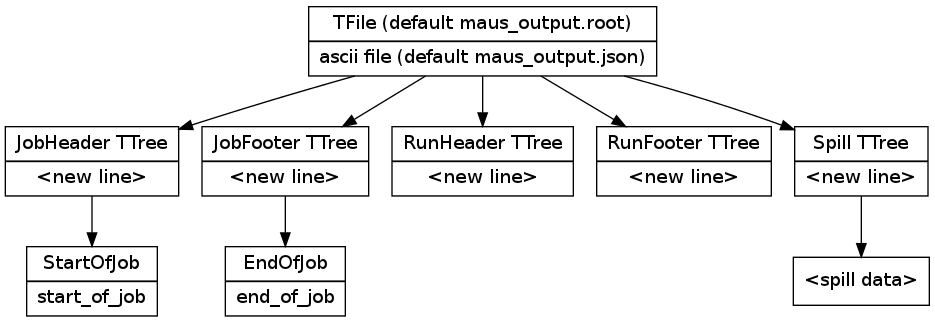
\includegraphics[width=0.9\textwidth]{file_structure.png}
\caption{The MAUS file structure including metadata. The top label in each box describes the representation in C++/ROOT. The bottom label describes the representation in JSON.}
\end{figure}


\section{The Spill Datastructure}
The major part of the MAUS data structure therefore is a tree of which each entry corresponds to the data associated with one spill. The spill is separated into three main sections: the MCEventArray contains an array of data each member of which represents the Monte Carlo of a single primary particle crossing the system; the ReconEventArray contains an array of data each member of which corresponds to a particle event (i.e. set of DAQ triggers); and the DAQData corresponds to the raw data readout. Additionally there are branches for reconstructed scalars, which are handled spill by spill and EMR data, which also read out on the spill rather than event by event.

\begin{figure}[!htb]
\centering
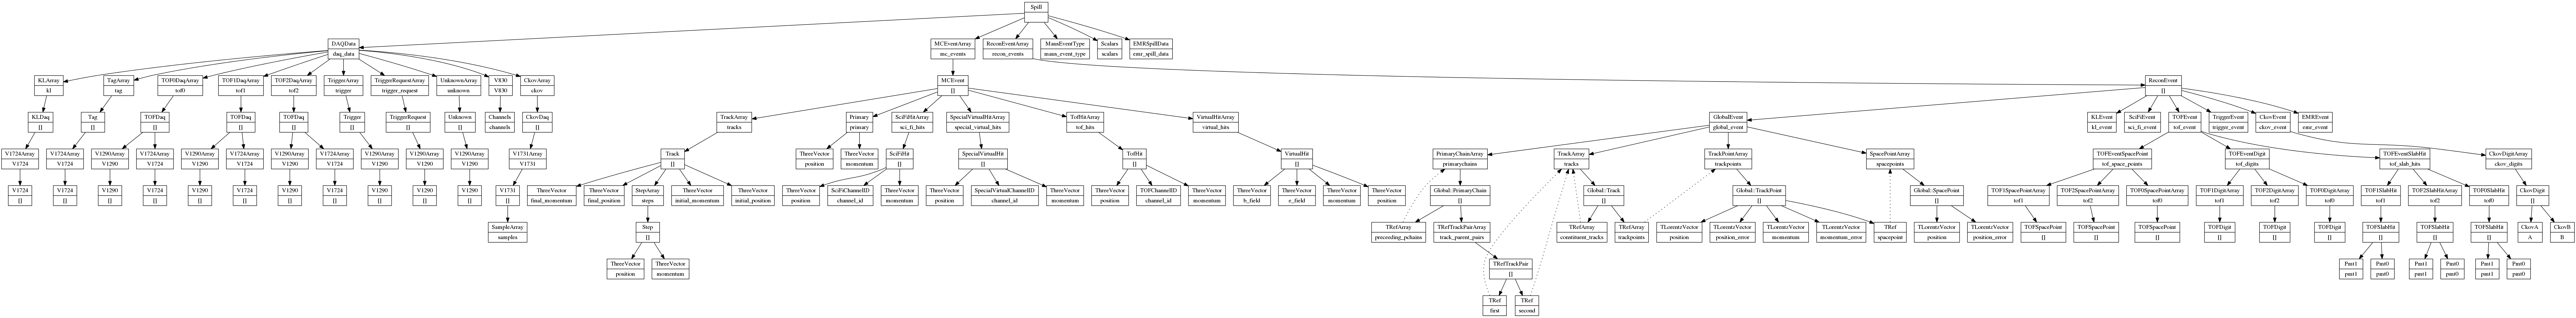
\includegraphics[width=0.9\textwidth]{spill_structure.png}
\caption{The MAUS output structure for a spill event. The top label in each box is the name of the C++ class and the bottom label is the json branch name. If a [] is shown, this indicates that child objects are array items.}
\end{figure}

The MCEvent is subdivided into sensitive detector hits and some pure Monte Carlo outputs. The primary that led to data being created is held in the Primary branch. Here the random seed, primary position momentum and so forth is stored. Sensitive detector hits have Hit data (energy deposited, position, momentum, etc) and a detector specific ChannelId that represents the channel of the detector that was hit - e.g. for TOF this indexes the slab, plane and station. Virtual hits are also stored - these are not sensitive detector hits, rather output position, momenta etc of particles that cross a particular plane in space, time or proper time is recorded. Note virtual hits do not inherit from the Hit class and have a slightly different data structure.

The ReconEvent and DAQEvents are subdivided by detector. ReconEvents contain reconstructed particle data for each detector and the trigger. There is an additional branch that contains global reconstruction output, that is the track fitting between detectors.

The data can be written in two formats. The main data format is a ROOT binary format. This requires the ROOT package to read and write, which is a standard analysis/plotting package in High Energy Physics and is installed by the MAUS build script. The secondary data format is JSON. This is an ascii data-tree format that in principle can be read by any text editor. Specific JSON parsers are also available - for example, the python \emph{json} module is available and comes prepackaged with MAUS.

\section{Accessing ROOT files}
For details on how to access the ROOT files, please see the introduction section of this document.

\section{Conversion to, and Working With, JSON}
MAUS also provides output in the JSON data format. This is an ascii format with IO libraries available for C++, Python and other languages. Two utilities are provided to perform conversions, \verb|bin/utilities/json_to_root.py| and \verb|bin/utilities/root_to_json.py| for conversion from and to JSON format respectively. JSON Input and Output modules are provided, \verb|InputPyJson| and \verb|OutputPyJson|.

An example json analysis is available in \verb|bin/examples/load_json_file.py|/

\section{Extending the Data Structure}
The data structure can be extended in MAUS by adding extra classes to the existing data structure. The data classes are in \verb|src/common_cpp/DataStructure|. In order to make these classes accessible to ROOT, the following steps must be taken:
\begin{itemize}
\item Add a new class in \verb|src/common_cpp/DataStructure|.
\item Ensure that default constructor, copy constructor, equality operator and destructor is present. The destructor must be virtual.
\item Make a typedef for each type of STL object you wish to use. ROOT does not handle STL objects terribly well otherwise. Even then there are limitations, for example accessing STL vector objects can cause a segmentation fault in PyROOT. Specific accessors are required to access data from STL objects for PyROOT interface.
\item Add a call to the ClassDef() macro at the end of the class definition before the closing braces. The ClassDef() macro is defined by the ROOT \verb|Rtypes.h| header file, and generates metaclasses based on information in the class which is put into the (dynamically generated) \verb|MausDataStructure.h| class.
\item Add the class to the list of classes in \verb|src/common_cpp/DataStructure/LinkDef.hh|. This is required for the class to be linked properly to the main library, and a linker error will result if this step is not taken.
\end{itemize}
In order to make these classes accessible to JSON, it is necessary to add a new processor in \verb|src/common_cpp/JsonCppProcessors|. There are a few default processors available.
\begin{itemize}
\item \verb|src/common_cpp/JsonCppProcessors/ProcessorBase.hh| contains IProcessor pure interface class for all processors and ProcessorBase base class (which may contain some implementation)
\item \verb|src/common_cpp/JsonCppProcessors/PrimitivesProcessors.hh| contains processors for primitive types; BoolProcessor, IntProcessor, UIntProcessor, StringProcessor, DoubleProcessor
\item \verb|src/common_cpp/JsonCppProcessors/ArrayProcessors.hh| contains processors for array types. Two processors are available: PointerArrayProcessor which converts an STL vector of pointers to data; and ValueArrayProcessor which converts an STL vector of values to data.
\item \verb|src/common_cpp/JsonCppProcessors/ObjectProcessor.hh| contains a processor for object types. Most of the classes in the MAUS data structure are represented in JSON as objects (string value pairs) where each string names a branch and each value contains data, which may be another class.
\item \verb|src/common_cpp/JsonCppProcessors/ObjectMapProcessors.hh| contains a processor for converting from JSON objects to STL maps. This is useful for JSON objects that contain lots of branches all of the same type.
\end{itemize}

A script, \verb|bin/user/json_branch_to_data_structure_and_cpp_processor.py| is available that analyses a JSON object or JSON tree of nested objects and converts to C++ classes. The script is provided "as-is" and it is expected that developers will check the output, adding comments and tests where appropriate.

\subsection{Pointer Handling}
MAUS can handle pointers for arrays and classes using ROOT native support or a reduced version compliant with the standard JSON reference syntax, where paths are indexed relative to the root value of a JSON document. JSON references are formatted like URIs, for example the JSON object \verb|{"$ref":"#spill/recon_events/1"}| would index the second recon_event in the spill object (indexing from 0). MAUS can only handle paths relative to the top level of the JSON document. In MAUS, it is necessary to make a distinction between data that is stored as a value in C++, data that is stored as a pointer in C++ and a pointer reference - that is a C++ pointer that references some pointer-as-data defined elsewhere in the data structure.

Conversion from C++ pointers to JSON pointers is handled in a type-safe way. Values-as-data are stored in the data tree converted at run time from JSON to C++ and vice versa. Pointers-as-data are handled in the same way as Values-as-data, but additionally an STL map is made. When converting from C++ to JSON, a map from the C++ pointer to the address of the JSON data is stored; when converting from JSON to C++ the map is in the opposite direction. The 

JSON stores pointers as references to other parts of the data tree. This is implemented in MAUS as two concepts - when a C++ \emph{pointer} is converted to JSON, the data is stored in an STL map that maps the C++ pointer to the JSON address. JSON \emph{references} to a pointer is placed into an STL vector of references together with the path to the JSON reference. After the tree has been parsed, MAUS iterates over the vector of references and for each reference stored it looks up the JSON address and places this as a reference into the JSON tree. The conversion is fully templated and abstracted to ensure type safety. Conversion from JSON pointers to C++ pointers is handled similarly, except: the map must operate in the opposite direction, from JSON address to C++ pointer; and the vector must now store the JSON address of the reference, together with the (instantiated) C++ object and the mutator that would set the reference.

 

\definecolor{AliceBlue}{rgb}{0.94,0.97,1.00}
\definecolor{AntiqueWhite1}{rgb}{1.00,0.94,0.86}
\definecolor{AntiqueWhite2}{rgb}{0.93,0.87,0.80}
\definecolor{AntiqueWhite3}{rgb}{0.80,0.75,0.69}
\definecolor{AntiqueWhite4}{rgb}{0.55,0.51,0.47}
\definecolor{AntiqueWhite}{rgb}{0.98,0.92,0.84}
\definecolor{BlanchedAlmond}{rgb}{1.00,0.92,0.80}
\definecolor{BlueViolet}{rgb}{0.54,0.17,0.89}
\definecolor{CadetBlue1}{rgb}{0.60,0.96,1.00}
\definecolor{CadetBlue2}{rgb}{0.56,0.90,0.93}
\definecolor{CadetBlue3}{rgb}{0.48,0.77,0.80}
\definecolor{CadetBlue4}{rgb}{0.33,0.53,0.55}
\definecolor{CadetBlue}{rgb}{0.37,0.62,0.63}
\definecolor{CornflowerBlue}{rgb}{0.39,0.58,0.93}
\definecolor{DarkBlue}{rgb}{0.00,0.00,0.55}
\definecolor{DarkCyan}{rgb}{0.00,0.55,0.55}
\definecolor{DarkGoldenrod1}{rgb}{1.00,0.73,0.06}
\definecolor{DarkGoldenrod2}{rgb}{0.93,0.68,0.05}
\definecolor{DarkGoldenrod3}{rgb}{0.80,0.58,0.05}
\definecolor{DarkGoldenrod4}{rgb}{0.55,0.40,0.03}
\definecolor{DarkGoldenrod}{rgb}{0.72,0.53,0.04}
\definecolor{DarkGray}{rgb}{0.66,0.66,0.66}
\definecolor{DarkGreen}{rgb}{0.00,0.39,0.00}
\definecolor{DarkGrey}{rgb}{0.66,0.66,0.66}
\definecolor{DarkKhaki}{rgb}{0.74,0.72,0.42}
\definecolor{DarkMagenta}{rgb}{0.55,0.00,0.55}
\definecolor{DarkOliveGreen1}{rgb}{0.79,1.00,0.44}
\definecolor{DarkOliveGreen2}{rgb}{0.74,0.93,0.41}
\definecolor{DarkOliveGreen3}{rgb}{0.64,0.80,0.35}
\definecolor{DarkOliveGreen4}{rgb}{0.43,0.55,0.24}
\definecolor{DarkOliveGreen}{rgb}{0.33,0.42,0.18}
\definecolor{DarkOrange1}{rgb}{1.00,0.50,0.00}
\definecolor{DarkOrange2}{rgb}{0.93,0.46,0.00}
\definecolor{DarkOrange3}{rgb}{0.80,0.40,0.00}
\definecolor{DarkOrange4}{rgb}{0.55,0.27,0.00}
\definecolor{DarkOrange}{rgb}{1.00,0.55,0.00}
\definecolor{DarkOrchid1}{rgb}{0.75,0.24,1.00}
\definecolor{DarkOrchid2}{rgb}{0.70,0.23,0.93}
\definecolor{DarkOrchid3}{rgb}{0.60,0.20,0.80}
\definecolor{DarkOrchid4}{rgb}{0.41,0.13,0.55}
\definecolor{DarkOrchid}{rgb}{0.60,0.20,0.80}
\definecolor{DarkRed}{rgb}{0.55,0.00,0.00}
\definecolor{DarkSalmon}{rgb}{0.91,0.59,0.48}
\definecolor{DarkSeaGreen1}{rgb}{0.76,1.00,0.76}
\definecolor{DarkSeaGreen2}{rgb}{0.71,0.93,0.71}
\definecolor{DarkSeaGreen3}{rgb}{0.61,0.80,0.61}
\definecolor{DarkSeaGreen4}{rgb}{0.41,0.55,0.41}
\definecolor{DarkSeaGreen}{rgb}{0.56,0.74,0.56}
\definecolor{DarkSlateBlue}{rgb}{0.28,0.24,0.55}
\definecolor{DarkSlateGray1}{rgb}{0.59,1.00,1.00}
\definecolor{DarkSlateGray2}{rgb}{0.55,0.93,0.93}
\definecolor{DarkSlateGray3}{rgb}{0.47,0.80,0.80}
\definecolor{DarkSlateGray4}{rgb}{0.32,0.55,0.55}
\definecolor{DarkSlateGray}{rgb}{0.18,0.31,0.31}
\definecolor{DarkSlateGrey}{rgb}{0.18,0.31,0.31}
\definecolor{DarkTurquoise}{rgb}{0.00,0.81,0.82}
\definecolor{DarkViolet}{rgb}{0.58,0.00,0.83}
\definecolor{DeepPink1}{rgb}{1.00,0.08,0.58}
\definecolor{DeepPink2}{rgb}{0.93,0.07,0.54}
\definecolor{DeepPink3}{rgb}{0.80,0.06,0.46}
\definecolor{DeepPink4}{rgb}{0.55,0.04,0.31}
\definecolor{DeepPink}{rgb}{1.00,0.08,0.58}
\definecolor{DeepSkyBlue1}{rgb}{0.00,0.75,1.00}
\definecolor{DeepSkyBlue2}{rgb}{0.00,0.70,0.93}
\definecolor{DeepSkyBlue3}{rgb}{0.00,0.60,0.80}
\definecolor{DeepSkyBlue4}{rgb}{0.00,0.41,0.55}
\definecolor{DeepSkyBlue}{rgb}{0.00,0.75,1.00}
\definecolor{DimGray}{rgb}{0.41,0.41,0.41}
\definecolor{DimGrey}{rgb}{0.41,0.41,0.41}
\definecolor{DodgerBlue1}{rgb}{0.12,0.56,1.00}
\definecolor{DodgerBlue2}{rgb}{0.11,0.53,0.93}
\definecolor{DodgerBlue3}{rgb}{0.09,0.45,0.80}
\definecolor{DodgerBlue4}{rgb}{0.06,0.31,0.55}
\definecolor{DodgerBlue}{rgb}{0.12,0.56,1.00}
\definecolor{FloralWhite}{rgb}{1.00,0.98,0.94}
\definecolor{ForestGreen}{rgb}{0.13,0.55,0.13}
\definecolor{GhostWhite}{rgb}{0.97,0.97,1.00}
\definecolor{GreenYellow}{rgb}{0.68,1.00,0.18}
\definecolor{HotPink1}{rgb}{1.00,0.43,0.71}
\definecolor{HotPink2}{rgb}{0.93,0.42,0.65}
\definecolor{HotPink3}{rgb}{0.80,0.38,0.56}
\definecolor{HotPink4}{rgb}{0.55,0.23,0.38}
\definecolor{HotPink}{rgb}{1.00,0.41,0.71}
\definecolor{IndianRed1}{rgb}{1.00,0.42,0.42}
\definecolor{IndianRed2}{rgb}{0.93,0.39,0.39}
\definecolor{IndianRed3}{rgb}{0.80,0.33,0.33}
\definecolor{IndianRed4}{rgb}{0.55,0.23,0.23}
\definecolor{IndianRed}{rgb}{0.80,0.36,0.36}
\definecolor{LavenderBlush1}{rgb}{1.00,0.94,0.96}
\definecolor{LavenderBlush2}{rgb}{0.93,0.88,0.90}
\definecolor{LavenderBlush3}{rgb}{0.80,0.76,0.77}
\definecolor{LavenderBlush4}{rgb}{0.55,0.51,0.53}
\definecolor{LavenderBlush}{rgb}{1.00,0.94,0.96}
\definecolor{LawnGreen}{rgb}{0.49,0.99,0.00}
\definecolor{LemonChiffon1}{rgb}{1.00,0.98,0.80}
\definecolor{LemonChiffon2}{rgb}{0.93,0.91,0.75}
\definecolor{LemonChiffon3}{rgb}{0.80,0.79,0.65}
\definecolor{LemonChiffon4}{rgb}{0.55,0.54,0.44}
\definecolor{LemonChiffon}{rgb}{1.00,0.98,0.80}
\definecolor{LightBlue1}{rgb}{0.75,0.94,1.00}
\definecolor{LightBlue2}{rgb}{0.70,0.87,0.93}
\definecolor{LightBlue3}{rgb}{0.60,0.75,0.80}
\definecolor{LightBlue4}{rgb}{0.41,0.51,0.55}
\definecolor{LightBlue}{rgb}{0.68,0.85,0.90}
\definecolor{LightCoral}{rgb}{0.94,0.50,0.50}
\definecolor{LightCyan1}{rgb}{0.88,1.00,1.00}
\definecolor{LightCyan2}{rgb}{0.82,0.93,0.93}
\definecolor{LightCyan3}{rgb}{0.71,0.80,0.80}
\definecolor{LightCyan4}{rgb}{0.48,0.55,0.55}
\definecolor{LightCyan}{rgb}{0.88,1.00,1.00}
\definecolor{LightGoldenrod1}{rgb}{1.00,0.93,0.55}
\definecolor{LightGoldenrod2}{rgb}{0.93,0.86,0.51}
\definecolor{LightGoldenrod3}{rgb}{0.80,0.75,0.44}
\definecolor{LightGoldenrod4}{rgb}{0.55,0.51,0.30}
\definecolor{LightGoldenrodYellow}{rgb}{0.98,0.98,0.82}
\definecolor{LightGoldenrod}{rgb}{0.93,0.87,0.51}
\definecolor{LightGray}{rgb}{0.83,0.83,0.83}
\definecolor{LightGreen}{rgb}{0.56,0.93,0.56}
\definecolor{LightGrey}{rgb}{0.83,0.83,0.83}
\definecolor{LightPink1}{rgb}{1.00,0.68,0.73}
\definecolor{LightPink2}{rgb}{0.93,0.64,0.68}
\definecolor{LightPink3}{rgb}{0.80,0.55,0.58}
\definecolor{LightPink4}{rgb}{0.55,0.37,0.40}
\definecolor{LightPink}{rgb}{1.00,0.71,0.76}
\definecolor{LightSalmon1}{rgb}{1.00,0.63,0.48}
\definecolor{LightSalmon2}{rgb}{0.93,0.58,0.45}
\definecolor{LightSalmon3}{rgb}{0.80,0.51,0.38}
\definecolor{LightSalmon4}{rgb}{0.55,0.34,0.26}
\definecolor{LightSalmon}{rgb}{1.00,0.63,0.48}
\definecolor{LightSeaGreen}{rgb}{0.13,0.70,0.67}
\definecolor{LightSkyBlue1}{rgb}{0.69,0.89,1.00}
\definecolor{LightSkyBlue2}{rgb}{0.64,0.83,0.93}
\definecolor{LightSkyBlue3}{rgb}{0.55,0.71,0.80}
\definecolor{LightSkyBlue4}{rgb}{0.38,0.48,0.55}
\definecolor{LightSkyBlue}{rgb}{0.53,0.81,0.98}
\definecolor{LightSlateBlue}{rgb}{0.52,0.44,1.00}
\definecolor{LightSlateGray}{rgb}{0.47,0.53,0.60}
\definecolor{LightSlateGrey}{rgb}{0.47,0.53,0.60}
\definecolor{LightSteelBlue1}{rgb}{0.79,0.88,1.00}
\definecolor{LightSteelBlue2}{rgb}{0.74,0.82,0.93}
\definecolor{LightSteelBlue3}{rgb}{0.64,0.71,0.80}
\definecolor{LightSteelBlue4}{rgb}{0.43,0.48,0.55}
\definecolor{LightSteelBlue}{rgb}{0.69,0.77,0.87}
\definecolor{LightYellow1}{rgb}{1.00,1.00,0.88}
\definecolor{LightYellow2}{rgb}{0.93,0.93,0.82}
\definecolor{LightYellow3}{rgb}{0.80,0.80,0.71}
\definecolor{LightYellow4}{rgb}{0.55,0.55,0.48}
\definecolor{LightYellow}{rgb}{1.00,1.00,0.88}
\definecolor{LimeGreen}{rgb}{0.20,0.80,0.20}
\definecolor{MediumAquamarine}{rgb}{0.40,0.80,0.67}
\definecolor{MediumBlue}{rgb}{0.00,0.00,0.80}
\definecolor{MediumOrchid1}{rgb}{0.88,0.40,1.00}
\definecolor{MediumOrchid2}{rgb}{0.82,0.37,0.93}
\definecolor{MediumOrchid3}{rgb}{0.71,0.32,0.80}
\definecolor{MediumOrchid4}{rgb}{0.48,0.22,0.55}
\definecolor{MediumOrchid}{rgb}{0.73,0.33,0.83}
\definecolor{MediumPurple1}{rgb}{0.67,0.51,1.00}
\definecolor{MediumPurple2}{rgb}{0.62,0.47,0.93}
\definecolor{MediumPurple3}{rgb}{0.54,0.41,0.80}
\definecolor{MediumPurple4}{rgb}{0.36,0.28,0.55}
\definecolor{MediumPurple}{rgb}{0.58,0.44,0.86}
\definecolor{MediumSeaGreen}{rgb}{0.24,0.70,0.44}
\definecolor{MediumSlateBlue}{rgb}{0.48,0.41,0.93}
\definecolor{MediumSpringGreen}{rgb}{0.00,0.98,0.60}
\definecolor{MediumTurquoise}{rgb}{0.28,0.82,0.80}
\definecolor{MediumVioletRed}{rgb}{0.78,0.08,0.52}
\definecolor{MidnightBlue}{rgb}{0.10,0.10,0.44}
\definecolor{MintCream}{rgb}{0.96,1.00,0.98}
\definecolor{MistyRose1}{rgb}{1.00,0.89,0.88}
\definecolor{MistyRose2}{rgb}{0.93,0.84,0.82}
\definecolor{MistyRose3}{rgb}{0.80,0.72,0.71}
\definecolor{MistyRose4}{rgb}{0.55,0.49,0.48}
\definecolor{MistyRose}{rgb}{1.00,0.89,0.88}
\definecolor{NavajoWhite1}{rgb}{1.00,0.87,0.68}
\definecolor{NavajoWhite2}{rgb}{0.93,0.81,0.63}
\definecolor{NavajoWhite3}{rgb}{0.80,0.70,0.55}
\definecolor{NavajoWhite4}{rgb}{0.55,0.47,0.37}
\definecolor{NavajoWhite}{rgb}{1.00,0.87,0.68}
\definecolor{NavyBlue}{rgb}{0.00,0.00,0.50}
\definecolor{OldLace}{rgb}{0.99,0.96,0.90}
\definecolor{OliveDrab1}{rgb}{0.75,1.00,0.24}
\definecolor{OliveDrab2}{rgb}{0.70,0.93,0.23}
\definecolor{OliveDrab3}{rgb}{0.60,0.80,0.20}
\definecolor{OliveDrab4}{rgb}{0.41,0.55,0.13}
\definecolor{OliveDrab}{rgb}{0.42,0.56,0.14}
\definecolor{OrangeRed1}{rgb}{1.00,0.27,0.00}
\definecolor{OrangeRed2}{rgb}{0.93,0.25,0.00}
\definecolor{OrangeRed3}{rgb}{0.80,0.22,0.00}
\definecolor{OrangeRed4}{rgb}{0.55,0.15,0.00}
\definecolor{OrangeRed}{rgb}{1.00,0.27,0.00}
\definecolor{PaleGoldenrod}{rgb}{0.93,0.91,0.67}
\definecolor{PaleGreen1}{rgb}{0.60,1.00,0.60}
\definecolor{PaleGreen2}{rgb}{0.56,0.93,0.56}
\definecolor{PaleGreen3}{rgb}{0.49,0.80,0.49}
\definecolor{PaleGreen4}{rgb}{0.33,0.55,0.33}
\definecolor{PaleGreen}{rgb}{0.60,0.98,0.60}
\definecolor{PaleTurquoise1}{rgb}{0.73,1.00,1.00}
\definecolor{PaleTurquoise2}{rgb}{0.68,0.93,0.93}
\definecolor{PaleTurquoise3}{rgb}{0.59,0.80,0.80}
\definecolor{PaleTurquoise4}{rgb}{0.40,0.55,0.55}
\definecolor{PaleTurquoise}{rgb}{0.69,0.93,0.93}
\definecolor{PaleVioletRed1}{rgb}{1.00,0.51,0.67}
\definecolor{PaleVioletRed2}{rgb}{0.93,0.47,0.62}
\definecolor{PaleVioletRed3}{rgb}{0.80,0.41,0.54}
\definecolor{PaleVioletRed4}{rgb}{0.55,0.28,0.36}
\definecolor{PaleVioletRed}{rgb}{0.86,0.44,0.58}
\definecolor{PapayaWhip}{rgb}{1.00,0.94,0.84}
\definecolor{PeachPuff1}{rgb}{1.00,0.85,0.73}
\definecolor{PeachPuff2}{rgb}{0.93,0.80,0.68}
\definecolor{PeachPuff3}{rgb}{0.80,0.69,0.58}
\definecolor{PeachPuff4}{rgb}{0.55,0.47,0.40}
\definecolor{PeachPuff}{rgb}{1.00,0.85,0.73}
\definecolor{PowderBlue}{rgb}{0.69,0.88,0.90}
\definecolor{RosyBrown1}{rgb}{1.00,0.76,0.76}
\definecolor{RosyBrown2}{rgb}{0.93,0.71,0.71}
\definecolor{RosyBrown3}{rgb}{0.80,0.61,0.61}
\definecolor{RosyBrown4}{rgb}{0.55,0.41,0.41}
\definecolor{RosyBrown}{rgb}{0.74,0.56,0.56}
\definecolor{RoyalBlue1}{rgb}{0.28,0.46,1.00}
\definecolor{RoyalBlue2}{rgb}{0.26,0.43,0.93}
\definecolor{RoyalBlue3}{rgb}{0.23,0.37,0.80}
\definecolor{RoyalBlue4}{rgb}{0.15,0.25,0.55}
\definecolor{RoyalBlue}{rgb}{0.25,0.41,0.88}
\definecolor{SaddleBrown}{rgb}{0.55,0.27,0.07}
\definecolor{SandyBrown}{rgb}{0.96,0.64,0.38}
\definecolor{SeaGreen1}{rgb}{0.33,1.00,0.62}
\definecolor{SeaGreen2}{rgb}{0.31,0.93,0.58}
\definecolor{SeaGreen3}{rgb}{0.26,0.80,0.50}
\definecolor{SeaGreen4}{rgb}{0.18,0.55,0.34}
\definecolor{SeaGreen}{rgb}{0.18,0.55,0.34}
\definecolor{SkyBlue1}{rgb}{0.53,0.81,1.00}
\definecolor{SkyBlue2}{rgb}{0.49,0.75,0.93}
\definecolor{SkyBlue3}{rgb}{0.42,0.65,0.80}
\definecolor{SkyBlue4}{rgb}{0.29,0.44,0.55}
\definecolor{SkyBlue}{rgb}{0.53,0.81,0.92}
\definecolor{SlateBlue1}{rgb}{0.51,0.44,1.00}
\definecolor{SlateBlue2}{rgb}{0.48,0.40,0.93}
\definecolor{SlateBlue3}{rgb}{0.41,0.35,0.80}
\definecolor{SlateBlue4}{rgb}{0.28,0.24,0.55}
\definecolor{SlateBlue}{rgb}{0.42,0.35,0.80}
\definecolor{SlateGray1}{rgb}{0.78,0.89,1.00}
\definecolor{SlateGray2}{rgb}{0.73,0.83,0.93}
\definecolor{SlateGray3}{rgb}{0.62,0.71,0.80}
\definecolor{SlateGray4}{rgb}{0.42,0.48,0.55}
\definecolor{SlateGray}{rgb}{0.44,0.50,0.56}
\definecolor{SlateGrey}{rgb}{0.44,0.50,0.56}
\definecolor{SpringGreen1}{rgb}{0.00,1.00,0.50}
\definecolor{SpringGreen2}{rgb}{0.00,0.93,0.46}
\definecolor{SpringGreen3}{rgb}{0.00,0.80,0.40}
\definecolor{SpringGreen4}{rgb}{0.00,0.55,0.27}
\definecolor{SpringGreen}{rgb}{0.00,1.00,0.50}
\definecolor{SteelBlue1}{rgb}{0.39,0.72,1.00}
\definecolor{SteelBlue2}{rgb}{0.36,0.67,0.93}
\definecolor{SteelBlue3}{rgb}{0.31,0.58,0.80}
\definecolor{SteelBlue4}{rgb}{0.21,0.39,0.55}
\definecolor{SteelBlue}{rgb}{0.27,0.51,0.71}
\definecolor{VioletRed1}{rgb}{1.00,0.24,0.59}
\definecolor{VioletRed2}{rgb}{0.93,0.23,0.55}
\definecolor{VioletRed3}{rgb}{0.80,0.20,0.47}
\definecolor{VioletRed4}{rgb}{0.55,0.13,0.32}
\definecolor{VioletRed}{rgb}{0.82,0.13,0.56}
\definecolor{WhiteSmoke}{rgb}{0.96,0.96,0.96}
\definecolor{YellowGreen}{rgb}{0.60,0.80,0.20}
\definecolor{aliceblue}{rgb}{0.94,0.97,1.00}
\definecolor{antiquewhite}{rgb}{0.98,0.92,0.84}
\definecolor{aquamarine1}{rgb}{0.50,1.00,0.83}
\definecolor{aquamarine2}{rgb}{0.46,0.93,0.78}
\definecolor{aquamarine3}{rgb}{0.40,0.80,0.67}
\definecolor{aquamarine4}{rgb}{0.27,0.55,0.45}
\definecolor{aquamarine}{rgb}{0.50,1.00,0.83}
\definecolor{azure1}{rgb}{0.94,1.00,1.00}
\definecolor{azure2}{rgb}{0.88,0.93,0.93}
\definecolor{azure3}{rgb}{0.76,0.80,0.80}
\definecolor{azure4}{rgb}{0.51,0.55,0.55}
\definecolor{azure}{rgb}{0.94,1.00,1.00}
\definecolor{beige}{rgb}{0.96,0.96,0.86}
\definecolor{bisque1}{rgb}{1.00,0.89,0.77}
\definecolor{bisque2}{rgb}{0.93,0.84,0.72}
\definecolor{bisque3}{rgb}{0.80,0.72,0.62}
\definecolor{bisque4}{rgb}{0.55,0.49,0.42}
\definecolor{bisque}{rgb}{1.00,0.89,0.77}
\definecolor{black}{rgb}{0.00,0.00,0.00}
\definecolor{blanchedalmond}{rgb}{1.00,0.92,0.80}
\definecolor{blue1}{rgb}{0.00,0.00,1.00}
\definecolor{blue2}{rgb}{0.00,0.00,0.93}
\definecolor{blue3}{rgb}{0.00,0.00,0.80}
\definecolor{blue4}{rgb}{0.00,0.00,0.55}
\definecolor{blueviolet}{rgb}{0.54,0.17,0.89}
\definecolor{blue}{rgb}{0.00,0.00,1.00}
\definecolor{brown1}{rgb}{1.00,0.25,0.25}
\definecolor{brown2}{rgb}{0.93,0.23,0.23}
\definecolor{brown3}{rgb}{0.80,0.20,0.20}
\definecolor{brown4}{rgb}{0.55,0.14,0.14}
\definecolor{brown}{rgb}{0.65,0.16,0.16}
\definecolor{burlywood1}{rgb}{1.00,0.83,0.61}
\definecolor{burlywood2}{rgb}{0.93,0.77,0.57}
\definecolor{burlywood3}{rgb}{0.80,0.67,0.49}
\definecolor{burlywood4}{rgb}{0.55,0.45,0.33}
\definecolor{burlywood}{rgb}{0.87,0.72,0.53}
\definecolor{cadetblue}{rgb}{0.37,0.62,0.63}
\definecolor{chartreuse1}{rgb}{0.50,1.00,0.00}
\definecolor{chartreuse2}{rgb}{0.46,0.93,0.00}
\definecolor{chartreuse3}{rgb}{0.40,0.80,0.00}
\definecolor{chartreuse4}{rgb}{0.27,0.55,0.00}
\definecolor{chartreuse}{rgb}{0.50,1.00,0.00}
\definecolor{chocolate1}{rgb}{1.00,0.50,0.14}
\definecolor{chocolate2}{rgb}{0.93,0.46,0.13}
\definecolor{chocolate3}{rgb}{0.80,0.40,0.11}
\definecolor{chocolate4}{rgb}{0.55,0.27,0.07}
\definecolor{chocolate}{rgb}{0.82,0.41,0.12}
\definecolor{coral1}{rgb}{1.00,0.45,0.34}
\definecolor{coral2}{rgb}{0.93,0.42,0.31}
\definecolor{coral3}{rgb}{0.80,0.36,0.27}
\definecolor{coral4}{rgb}{0.55,0.24,0.18}
\definecolor{coral}{rgb}{1.00,0.50,0.31}
\definecolor{cornflowerblue}{rgb}{0.39,0.58,0.93}
\definecolor{cornsilk1}{rgb}{1.00,0.97,0.86}
\definecolor{cornsilk2}{rgb}{0.93,0.91,0.80}
\definecolor{cornsilk3}{rgb}{0.80,0.78,0.69}
\definecolor{cornsilk4}{rgb}{0.55,0.53,0.47}
\definecolor{cornsilk}{rgb}{1.00,0.97,0.86}
\definecolor{cyan1}{rgb}{0.00,1.00,1.00}
\definecolor{cyan2}{rgb}{0.00,0.93,0.93}
\definecolor{cyan3}{rgb}{0.00,0.80,0.80}
\definecolor{cyan4}{rgb}{0.00,0.55,0.55}
\definecolor{cyan}{rgb}{0.00,1.00,1.00}
\definecolor{darkblue}{rgb}{0.00,0.00,0.55}
\definecolor{darkcyan}{rgb}{0.00,0.55,0.55}
\definecolor{darkgoldenrod}{rgb}{0.72,0.53,0.04}
\definecolor{darkgray}{rgb}{0.66,0.66,0.66}
\definecolor{darkgreen}{rgb}{0.00,0.39,0.00}
\definecolor{darkgrey}{rgb}{0.66,0.66,0.66}
\definecolor{darkkhaki}{rgb}{0.74,0.72,0.42}
\definecolor{darkmagenta}{rgb}{0.55,0.00,0.55}
\definecolor{darkolive}{rgb}{0.33,0.42,0.18}
\definecolor{darkorange}{rgb}{1.00,0.55,0.00}
\definecolor{darkorchid}{rgb}{0.60,0.20,0.80}
\definecolor{darkred}{rgb}{0.55,0.00,0.00}
\definecolor{darksalmon}{rgb}{0.91,0.59,0.48}
\definecolor{darksea}{rgb}{0.56,0.74,0.56}
\definecolor{darkslate}{rgb}{0.18,0.31,0.31}
\definecolor{darkslate}{rgb}{0.18,0.31,0.31}
\definecolor{darkslate}{rgb}{0.28,0.24,0.55}
\definecolor{darkturquoise}{rgb}{0.00,0.81,0.82}
\definecolor{darkviolet}{rgb}{0.58,0.00,0.83}
\definecolor{deeppink}{rgb}{1.00,0.08,0.58}
\definecolor{deepsky}{rgb}{0.00,0.75,1.00}
\definecolor{dimgray}{rgb}{0.41,0.41,0.41}
\definecolor{dimgrey}{rgb}{0.41,0.41,0.41}
\definecolor{dodgerblue}{rgb}{0.12,0.56,1.00}
\definecolor{firebrick1}{rgb}{1.00,0.19,0.19}
\definecolor{firebrick2}{rgb}{0.93,0.17,0.17}
\definecolor{firebrick3}{rgb}{0.80,0.15,0.15}
\definecolor{firebrick4}{rgb}{0.55,0.10,0.10}
\definecolor{firebrick}{rgb}{0.70,0.13,0.13}
\definecolor{floralwhite}{rgb}{1.00,0.98,0.94}
\definecolor{forestgreen}{rgb}{0.13,0.55,0.13}
\definecolor{gainsboro}{rgb}{0.86,0.86,0.86}
\definecolor{ghostwhite}{rgb}{0.97,0.97,1.00}
\definecolor{gold1}{rgb}{1.00,0.84,0.00}
\definecolor{gold2}{rgb}{0.93,0.79,0.00}
\definecolor{gold3}{rgb}{0.80,0.68,0.00}
\definecolor{gold4}{rgb}{0.55,0.46,0.00}
\definecolor{goldenrod1}{rgb}{1.00,0.76,0.15}
\definecolor{goldenrod2}{rgb}{0.93,0.71,0.13}
\definecolor{goldenrod3}{rgb}{0.80,0.61,0.11}
\definecolor{goldenrod4}{rgb}{0.55,0.41,0.08}
\definecolor{goldenrod}{rgb}{0.85,0.65,0.13}
\definecolor{gold}{rgb}{1.00,0.84,0.00}
\definecolor{gray0}{rgb}{0.00,0.00,0.00}
\definecolor{gray100}{rgb}{1.00,1.00,1.00}
\definecolor{gray10}{rgb}{0.10,0.10,0.10}
\definecolor{gray11}{rgb}{0.11,0.11,0.11}
\definecolor{gray12}{rgb}{0.12,0.12,0.12}
\definecolor{gray13}{rgb}{0.13,0.13,0.13}
\definecolor{gray14}{rgb}{0.14,0.14,0.14}
\definecolor{gray15}{rgb}{0.15,0.15,0.15}
\definecolor{gray16}{rgb}{0.16,0.16,0.16}
\definecolor{gray17}{rgb}{0.17,0.17,0.17}
\definecolor{gray18}{rgb}{0.18,0.18,0.18}
\definecolor{gray19}{rgb}{0.19,0.19,0.19}
\definecolor{gray1}{rgb}{0.01,0.01,0.01}
\definecolor{gray20}{rgb}{0.20,0.20,0.20}
\definecolor{gray21}{rgb}{0.21,0.21,0.21}
\definecolor{gray22}{rgb}{0.22,0.22,0.22}
\definecolor{gray23}{rgb}{0.23,0.23,0.23}
\definecolor{gray24}{rgb}{0.24,0.24,0.24}
\definecolor{gray25}{rgb}{0.25,0.25,0.25}
\definecolor{gray26}{rgb}{0.26,0.26,0.26}
\definecolor{gray27}{rgb}{0.27,0.27,0.27}
\definecolor{gray28}{rgb}{0.28,0.28,0.28}
\definecolor{gray29}{rgb}{0.29,0.29,0.29}
\definecolor{gray2}{rgb}{0.02,0.02,0.02}
\definecolor{gray30}{rgb}{0.30,0.30,0.30}
\definecolor{gray31}{rgb}{0.31,0.31,0.31}
\definecolor{gray32}{rgb}{0.32,0.32,0.32}
\definecolor{gray33}{rgb}{0.33,0.33,0.33}
\definecolor{gray34}{rgb}{0.34,0.34,0.34}
\definecolor{gray35}{rgb}{0.35,0.35,0.35}
\definecolor{gray36}{rgb}{0.36,0.36,0.36}
\definecolor{gray37}{rgb}{0.37,0.37,0.37}
\definecolor{gray38}{rgb}{0.38,0.38,0.38}
\definecolor{gray39}{rgb}{0.39,0.39,0.39}
\definecolor{gray3}{rgb}{0.03,0.03,0.03}
\definecolor{gray40}{rgb}{0.40,0.40,0.40}
\definecolor{gray41}{rgb}{0.41,0.41,0.41}
\definecolor{gray42}{rgb}{0.42,0.42,0.42}
\definecolor{gray43}{rgb}{0.43,0.43,0.43}
\definecolor{gray44}{rgb}{0.44,0.44,0.44}
\definecolor{gray45}{rgb}{0.45,0.45,0.45}
\definecolor{gray46}{rgb}{0.46,0.46,0.46}
\definecolor{gray47}{rgb}{0.47,0.47,0.47}
\definecolor{gray48}{rgb}{0.48,0.48,0.48}
\definecolor{gray49}{rgb}{0.49,0.49,0.49}
\definecolor{gray4}{rgb}{0.04,0.04,0.04}
\definecolor{gray50}{rgb}{0.50,0.50,0.50}
\definecolor{gray51}{rgb}{0.51,0.51,0.51}
\definecolor{gray52}{rgb}{0.52,0.52,0.52}
\definecolor{gray53}{rgb}{0.53,0.53,0.53}
\definecolor{gray54}{rgb}{0.54,0.54,0.54}
\definecolor{gray55}{rgb}{0.55,0.55,0.55}
\definecolor{gray56}{rgb}{0.56,0.56,0.56}
\definecolor{gray57}{rgb}{0.57,0.57,0.57}
\definecolor{gray58}{rgb}{0.58,0.58,0.58}
\definecolor{gray59}{rgb}{0.59,0.59,0.59}
\definecolor{gray5}{rgb}{0.05,0.05,0.05}
\definecolor{gray60}{rgb}{0.60,0.60,0.60}
\definecolor{gray61}{rgb}{0.61,0.61,0.61}
\definecolor{gray62}{rgb}{0.62,0.62,0.62}
\definecolor{gray63}{rgb}{0.63,0.63,0.63}
\definecolor{gray64}{rgb}{0.64,0.64,0.64}
\definecolor{gray65}{rgb}{0.65,0.65,0.65}
\definecolor{gray66}{rgb}{0.66,0.66,0.66}
\definecolor{gray67}{rgb}{0.67,0.67,0.67}
\definecolor{gray68}{rgb}{0.68,0.68,0.68}
\definecolor{gray69}{rgb}{0.69,0.69,0.69}
\definecolor{gray6}{rgb}{0.06,0.06,0.06}
\definecolor{gray70}{rgb}{0.70,0.70,0.70}
\definecolor{gray71}{rgb}{0.71,0.71,0.71}
\definecolor{gray72}{rgb}{0.72,0.72,0.72}
\definecolor{gray73}{rgb}{0.73,0.73,0.73}
\definecolor{gray74}{rgb}{0.74,0.74,0.74}
\definecolor{gray75}{rgb}{0.75,0.75,0.75}
\definecolor{gray76}{rgb}{0.76,0.76,0.76}
\definecolor{gray77}{rgb}{0.77,0.77,0.77}
\definecolor{gray78}{rgb}{0.78,0.78,0.78}
\definecolor{gray79}{rgb}{0.79,0.79,0.79}
\definecolor{gray7}{rgb}{0.07,0.07,0.07}
\definecolor{gray80}{rgb}{0.80,0.80,0.80}
\definecolor{gray81}{rgb}{0.81,0.81,0.81}
\definecolor{gray82}{rgb}{0.82,0.82,0.82}
\definecolor{gray83}{rgb}{0.83,0.83,0.83}
\definecolor{gray84}{rgb}{0.84,0.84,0.84}
\definecolor{gray85}{rgb}{0.85,0.85,0.85}
\definecolor{gray86}{rgb}{0.86,0.86,0.86}
\definecolor{gray87}{rgb}{0.87,0.87,0.87}
\definecolor{gray88}{rgb}{0.88,0.88,0.88}
\definecolor{gray89}{rgb}{0.89,0.89,0.89}
\definecolor{gray8}{rgb}{0.08,0.08,0.08}
\definecolor{gray90}{rgb}{0.90,0.90,0.90}
\definecolor{gray91}{rgb}{0.91,0.91,0.91}
\definecolor{gray92}{rgb}{0.92,0.92,0.92}
\definecolor{gray93}{rgb}{0.93,0.93,0.93}
\definecolor{gray94}{rgb}{0.94,0.94,0.94}
\definecolor{gray95}{rgb}{0.95,0.95,0.95}
\definecolor{gray96}{rgb}{0.96,0.96,0.96}
\definecolor{gray97}{rgb}{0.97,0.97,0.97}
\definecolor{gray98}{rgb}{0.98,0.98,0.98}
\definecolor{gray99}{rgb}{0.99,0.99,0.99}
\definecolor{gray9}{rgb}{0.09,0.09,0.09}
\definecolor{gray}{rgb}{0.75,0.75,0.75}
\definecolor{green1}{rgb}{0.00,1.00,0.00}
\definecolor{green2}{rgb}{0.00,0.93,0.00}
\definecolor{green3}{rgb}{0.00,0.80,0.00}
\definecolor{green4}{rgb}{0.00,0.55,0.00}
\definecolor{greenyellow}{rgb}{0.68,1.00,0.18}
\definecolor{green}{rgb}{0.00,1.00,0.00}
\definecolor{grey0}{rgb}{0.00,0.00,0.00}
\definecolor{grey100}{rgb}{1.00,1.00,1.00}
\definecolor{grey10}{rgb}{0.10,0.10,0.10}
\definecolor{grey11}{rgb}{0.11,0.11,0.11}
\definecolor{grey12}{rgb}{0.12,0.12,0.12}
\definecolor{grey13}{rgb}{0.13,0.13,0.13}
\definecolor{grey14}{rgb}{0.14,0.14,0.14}
\definecolor{grey15}{rgb}{0.15,0.15,0.15}
\definecolor{grey16}{rgb}{0.16,0.16,0.16}
\definecolor{grey17}{rgb}{0.17,0.17,0.17}
\definecolor{grey18}{rgb}{0.18,0.18,0.18}
\definecolor{grey19}{rgb}{0.19,0.19,0.19}
\definecolor{grey1}{rgb}{0.01,0.01,0.01}
\definecolor{grey20}{rgb}{0.20,0.20,0.20}
\definecolor{grey21}{rgb}{0.21,0.21,0.21}
\definecolor{grey22}{rgb}{0.22,0.22,0.22}
\definecolor{grey23}{rgb}{0.23,0.23,0.23}
\definecolor{grey24}{rgb}{0.24,0.24,0.24}
\definecolor{grey25}{rgb}{0.25,0.25,0.25}
\definecolor{grey26}{rgb}{0.26,0.26,0.26}
\definecolor{grey27}{rgb}{0.27,0.27,0.27}
\definecolor{grey28}{rgb}{0.28,0.28,0.28}
\definecolor{grey29}{rgb}{0.29,0.29,0.29}
\definecolor{grey2}{rgb}{0.02,0.02,0.02}
\definecolor{grey30}{rgb}{0.30,0.30,0.30}
\definecolor{grey31}{rgb}{0.31,0.31,0.31}
\definecolor{grey32}{rgb}{0.32,0.32,0.32}
\definecolor{grey33}{rgb}{0.33,0.33,0.33}
\definecolor{grey34}{rgb}{0.34,0.34,0.34}
\definecolor{grey35}{rgb}{0.35,0.35,0.35}
\definecolor{grey36}{rgb}{0.36,0.36,0.36}
\definecolor{grey37}{rgb}{0.37,0.37,0.37}
\definecolor{grey38}{rgb}{0.38,0.38,0.38}
\definecolor{grey39}{rgb}{0.39,0.39,0.39}
\definecolor{grey3}{rgb}{0.03,0.03,0.03}
\definecolor{grey40}{rgb}{0.40,0.40,0.40}
\definecolor{grey41}{rgb}{0.41,0.41,0.41}
\definecolor{grey42}{rgb}{0.42,0.42,0.42}
\definecolor{grey43}{rgb}{0.43,0.43,0.43}
\definecolor{grey44}{rgb}{0.44,0.44,0.44}
\definecolor{grey45}{rgb}{0.45,0.45,0.45}
\definecolor{grey46}{rgb}{0.46,0.46,0.46}
\definecolor{grey47}{rgb}{0.47,0.47,0.47}
\definecolor{grey48}{rgb}{0.48,0.48,0.48}
\definecolor{grey49}{rgb}{0.49,0.49,0.49}
\definecolor{grey4}{rgb}{0.04,0.04,0.04}
\definecolor{grey50}{rgb}{0.50,0.50,0.50}
\definecolor{grey51}{rgb}{0.51,0.51,0.51}
\definecolor{grey52}{rgb}{0.52,0.52,0.52}
\definecolor{grey53}{rgb}{0.53,0.53,0.53}
\definecolor{grey54}{rgb}{0.54,0.54,0.54}
\definecolor{grey55}{rgb}{0.55,0.55,0.55}
\definecolor{grey56}{rgb}{0.56,0.56,0.56}
\definecolor{grey57}{rgb}{0.57,0.57,0.57}
\definecolor{grey58}{rgb}{0.58,0.58,0.58}
\definecolor{grey59}{rgb}{0.59,0.59,0.59}
\definecolor{grey5}{rgb}{0.05,0.05,0.05}
\definecolor{grey60}{rgb}{0.60,0.60,0.60}
\definecolor{grey61}{rgb}{0.61,0.61,0.61}
\definecolor{grey62}{rgb}{0.62,0.62,0.62}
\definecolor{grey63}{rgb}{0.63,0.63,0.63}
\definecolor{grey64}{rgb}{0.64,0.64,0.64}
\definecolor{grey65}{rgb}{0.65,0.65,0.65}
\definecolor{grey66}{rgb}{0.66,0.66,0.66}
\definecolor{grey67}{rgb}{0.67,0.67,0.67}
\definecolor{grey68}{rgb}{0.68,0.68,0.68}
\definecolor{grey69}{rgb}{0.69,0.69,0.69}
\definecolor{grey6}{rgb}{0.06,0.06,0.06}
\definecolor{grey70}{rgb}{0.70,0.70,0.70}
\definecolor{grey71}{rgb}{0.71,0.71,0.71}
\definecolor{grey72}{rgb}{0.72,0.72,0.72}
\definecolor{grey73}{rgb}{0.73,0.73,0.73}
\definecolor{grey74}{rgb}{0.74,0.74,0.74}
\definecolor{grey75}{rgb}{0.75,0.75,0.75}
\definecolor{grey76}{rgb}{0.76,0.76,0.76}
\definecolor{grey77}{rgb}{0.77,0.77,0.77}
\definecolor{grey78}{rgb}{0.78,0.78,0.78}
\definecolor{grey79}{rgb}{0.79,0.79,0.79}
\definecolor{grey7}{rgb}{0.07,0.07,0.07}
\definecolor{grey80}{rgb}{0.80,0.80,0.80}
\definecolor{grey81}{rgb}{0.81,0.81,0.81}
\definecolor{grey82}{rgb}{0.82,0.82,0.82}
\definecolor{grey83}{rgb}{0.83,0.83,0.83}
\definecolor{grey84}{rgb}{0.84,0.84,0.84}
\definecolor{grey85}{rgb}{0.85,0.85,0.85}
\definecolor{grey86}{rgb}{0.86,0.86,0.86}
\definecolor{grey87}{rgb}{0.87,0.87,0.87}
\definecolor{grey88}{rgb}{0.88,0.88,0.88}
\definecolor{grey89}{rgb}{0.89,0.89,0.89}
\definecolor{grey8}{rgb}{0.08,0.08,0.08}
\definecolor{grey90}{rgb}{0.90,0.90,0.90}
\definecolor{grey91}{rgb}{0.91,0.91,0.91}
\definecolor{grey92}{rgb}{0.92,0.92,0.92}
\definecolor{grey93}{rgb}{0.93,0.93,0.93}
\definecolor{grey94}{rgb}{0.94,0.94,0.94}
\definecolor{grey95}{rgb}{0.95,0.95,0.95}
\definecolor{grey96}{rgb}{0.96,0.96,0.96}
\definecolor{grey97}{rgb}{0.97,0.97,0.97}
\definecolor{grey98}{rgb}{0.98,0.98,0.98}
\definecolor{grey99}{rgb}{0.99,0.99,0.99}
\definecolor{grey9}{rgb}{0.09,0.09,0.09}
\definecolor{grey}{rgb}{0.75,0.75,0.75}
\definecolor{honeydew1}{rgb}{0.94,1.00,0.94}
\definecolor{honeydew2}{rgb}{0.88,0.93,0.88}
\definecolor{honeydew3}{rgb}{0.76,0.80,0.76}
\definecolor{honeydew4}{rgb}{0.51,0.55,0.51}
\definecolor{honeydew}{rgb}{0.94,1.00,0.94}
\definecolor{hotpink}{rgb}{1.00,0.41,0.71}
\definecolor{indianred}{rgb}{0.80,0.36,0.36}
\definecolor{ivory1}{rgb}{1.00,1.00,0.94}
\definecolor{ivory2}{rgb}{0.93,0.93,0.88}
\definecolor{ivory3}{rgb}{0.80,0.80,0.76}
\definecolor{ivory4}{rgb}{0.55,0.55,0.51}
\definecolor{ivory}{rgb}{1.00,1.00,0.94}
\definecolor{khaki1}{rgb}{1.00,0.96,0.56}
\definecolor{khaki2}{rgb}{0.93,0.90,0.52}
\definecolor{khaki3}{rgb}{0.80,0.78,0.45}
\definecolor{khaki4}{rgb}{0.55,0.53,0.31}
\definecolor{khaki}{rgb}{0.94,0.90,0.55}
\definecolor{lavenderblush}{rgb}{1.00,0.94,0.96}
\definecolor{lavender}{rgb}{0.90,0.90,0.98}
\definecolor{lawngreen}{rgb}{0.49,0.99,0.00}
\definecolor{lemonchiffon}{rgb}{1.00,0.98,0.80}
\definecolor{lightblue}{rgb}{0.68,0.85,0.90}
\definecolor{lightcoral}{rgb}{0.94,0.50,0.50}
\definecolor{lightcyan}{rgb}{0.88,1.00,1.00}
\definecolor{lightgoldenrod}{rgb}{0.93,0.87,0.51}
\definecolor{lightgoldenrod}{rgb}{0.98,0.98,0.82}
\definecolor{lightgray}{rgb}{0.83,0.83,0.83}
\definecolor{lightgreen}{rgb}{0.56,0.93,0.56}
\definecolor{lightgrey}{rgb}{0.83,0.83,0.83}
\definecolor{lightpink}{rgb}{1.00,0.71,0.76}
\definecolor{lightsalmon}{rgb}{1.00,0.63,0.48}
\definecolor{lightsea}{rgb}{0.13,0.70,0.67}
\definecolor{lightsky}{rgb}{0.53,0.81,0.98}
\definecolor{lightslate}{rgb}{0.47,0.53,0.60}
\definecolor{lightslate}{rgb}{0.47,0.53,0.60}
\definecolor{lightslate}{rgb}{0.52,0.44,1.00}
\definecolor{lightsteel}{rgb}{0.69,0.77,0.87}
\definecolor{lightyellow}{rgb}{1.00,1.00,0.88}
\definecolor{limegreen}{rgb}{0.20,0.80,0.20}
\definecolor{linen}{rgb}{0.98,0.94,0.90}
\definecolor{magenta1}{rgb}{1.00,0.00,1.00}
\definecolor{magenta2}{rgb}{0.93,0.00,0.93}
\definecolor{magenta3}{rgb}{0.80,0.00,0.80}
\definecolor{magenta4}{rgb}{0.55,0.00,0.55}
\definecolor{magenta}{rgb}{1.00,0.00,1.00}
\definecolor{maroon1}{rgb}{1.00,0.20,0.70}
\definecolor{maroon2}{rgb}{0.93,0.19,0.65}
\definecolor{maroon3}{rgb}{0.80,0.16,0.56}
\definecolor{maroon4}{rgb}{0.55,0.11,0.38}
\definecolor{maroon}{rgb}{0.69,0.19,0.38}
\definecolor{mediumaquamarine}{rgb}{0.40,0.80,0.67}
\definecolor{mediumblue}{rgb}{0.00,0.00,0.80}
\definecolor{mediumorchid}{rgb}{0.73,0.33,0.83}
\definecolor{mediumpurple}{rgb}{0.58,0.44,0.86}
\definecolor{mediumsea}{rgb}{0.24,0.70,0.44}
\definecolor{mediumslate}{rgb}{0.48,0.41,0.93}
\definecolor{mediumspring}{rgb}{0.00,0.98,0.60}
\definecolor{mediumturquoise}{rgb}{0.28,0.82,0.80}
\definecolor{mediumviolet}{rgb}{0.78,0.08,0.52}
\definecolor{midnightblue}{rgb}{0.10,0.10,0.44}
\definecolor{mintcream}{rgb}{0.96,1.00,0.98}
\definecolor{mistyrose}{rgb}{1.00,0.89,0.88}
\definecolor{moccasin}{rgb}{1.00,0.89,0.71}
\definecolor{navajowhite}{rgb}{1.00,0.87,0.68}
\definecolor{navyblue}{rgb}{0.00,0.00,0.50}
\definecolor{navy}{rgb}{0.00,0.00,0.50}
\definecolor{oldlace}{rgb}{0.99,0.96,0.90}
\definecolor{olivedrab}{rgb}{0.42,0.56,0.14}
\definecolor{orange1}{rgb}{1.00,0.65,0.00}
\definecolor{orange2}{rgb}{0.93,0.60,0.00}
\definecolor{orange3}{rgb}{0.80,0.52,0.00}
\definecolor{orange4}{rgb}{0.55,0.35,0.00}
\definecolor{orangered}{rgb}{1.00,0.27,0.00}
\definecolor{orange}{rgb}{1.00,0.65,0.00}
\definecolor{orchid1}{rgb}{1.00,0.51,0.98}
\definecolor{orchid2}{rgb}{0.93,0.48,0.91}
\definecolor{orchid3}{rgb}{0.80,0.41,0.79}
\definecolor{orchid4}{rgb}{0.55,0.28,0.54}
\definecolor{orchid}{rgb}{0.85,0.44,0.84}
\definecolor{palegoldenrod}{rgb}{0.93,0.91,0.67}
\definecolor{palegreen}{rgb}{0.60,0.98,0.60}
\definecolor{paleturquoise}{rgb}{0.69,0.93,0.93}
\definecolor{paleviolet}{rgb}{0.86,0.44,0.58}
\definecolor{papayawhip}{rgb}{1.00,0.94,0.84}
\definecolor{peachpuff}{rgb}{1.00,0.85,0.73}
\definecolor{peru}{rgb}{0.80,0.52,0.25}
\definecolor{pink1}{rgb}{1.00,0.71,0.77}
\definecolor{pink2}{rgb}{0.93,0.66,0.72}
\definecolor{pink3}{rgb}{0.80,0.57,0.62}
\definecolor{pink4}{rgb}{0.55,0.39,0.42}
\definecolor{pink}{rgb}{1.00,0.75,0.80}
\definecolor{plum1}{rgb}{1.00,0.73,1.00}
\definecolor{plum2}{rgb}{0.93,0.68,0.93}
\definecolor{plum3}{rgb}{0.80,0.59,0.80}
\definecolor{plum4}{rgb}{0.55,0.40,0.55}
\definecolor{plum}{rgb}{0.87,0.63,0.87}
\definecolor{powderblue}{rgb}{0.69,0.88,0.90}
\definecolor{purple1}{rgb}{0.61,0.19,1.00}
\definecolor{purple2}{rgb}{0.57,0.17,0.93}
\definecolor{purple3}{rgb}{0.49,0.15,0.80}
\definecolor{purple4}{rgb}{0.33,0.10,0.55}
\definecolor{purple}{rgb}{0.63,0.13,0.94}
\definecolor{red1}{rgb}{1.00,0.00,0.00}
\definecolor{red2}{rgb}{0.93,0.00,0.00}
\definecolor{red3}{rgb}{0.80,0.00,0.00}
\definecolor{red4}{rgb}{0.55,0.00,0.00}
\definecolor{red}{rgb}{1.00,0.00,0.00}
\definecolor{rosybrown}{rgb}{0.74,0.56,0.56}
\definecolor{royalblue}{rgb}{0.25,0.41,0.88}
\definecolor{saddlebrown}{rgb}{0.55,0.27,0.07}
\definecolor{salmon1}{rgb}{1.00,0.55,0.41}
\definecolor{salmon2}{rgb}{0.93,0.51,0.38}
\definecolor{salmon3}{rgb}{0.80,0.44,0.33}
\definecolor{salmon4}{rgb}{0.55,0.30,0.22}
\definecolor{salmon}{rgb}{0.98,0.50,0.45}
\definecolor{sandybrown}{rgb}{0.96,0.64,0.38}
\definecolor{seagreen}{rgb}{0.18,0.55,0.34}
\definecolor{seashell1}{rgb}{1.00,0.96,0.93}
\definecolor{seashell2}{rgb}{0.93,0.90,0.87}
\definecolor{seashell3}{rgb}{0.80,0.77,0.75}
\definecolor{seashell4}{rgb}{0.55,0.53,0.51}
\definecolor{seashell}{rgb}{1.00,0.96,0.93}
\definecolor{sienna1}{rgb}{1.00,0.51,0.28}
\definecolor{sienna2}{rgb}{0.93,0.47,0.26}
\definecolor{sienna3}{rgb}{0.80,0.41,0.22}
\definecolor{sienna4}{rgb}{0.55,0.28,0.15}
\definecolor{sienna}{rgb}{0.63,0.32,0.18}
\definecolor{skyblue}{rgb}{0.53,0.81,0.92}
\definecolor{slateblue}{rgb}{0.42,0.35,0.80}
\definecolor{slategray}{rgb}{0.44,0.50,0.56}
\definecolor{slategrey}{rgb}{0.44,0.50,0.56}
\definecolor{snow1}{rgb}{1.00,0.98,0.98}
\definecolor{snow2}{rgb}{0.93,0.91,0.91}
\definecolor{snow3}{rgb}{0.80,0.79,0.79}
\definecolor{snow4}{rgb}{0.55,0.54,0.54}
\definecolor{snow}{rgb}{1.00,0.98,0.98}
\definecolor{springgreen}{rgb}{0.00,1.00,0.50}
\definecolor{steelblue}{rgb}{0.27,0.51,0.71}
\definecolor{tan1}{rgb}{1.00,0.65,0.31}
\definecolor{tan2}{rgb}{0.93,0.60,0.29}
\definecolor{tan3}{rgb}{0.80,0.52,0.25}
\definecolor{tan4}{rgb}{0.55,0.35,0.17}
\definecolor{tan}{rgb}{0.82,0.71,0.55}
\definecolor{thistle1}{rgb}{1.00,0.88,1.00}
\definecolor{thistle2}{rgb}{0.93,0.82,0.93}
\definecolor{thistle3}{rgb}{0.80,0.71,0.80}
\definecolor{thistle4}{rgb}{0.55,0.48,0.55}
\definecolor{thistle}{rgb}{0.85,0.75,0.85}
\definecolor{tomato1}{rgb}{1.00,0.39,0.28}
\definecolor{tomato2}{rgb}{0.93,0.36,0.26}
\definecolor{tomato3}{rgb}{0.80,0.31,0.22}
\definecolor{tomato4}{rgb}{0.55,0.21,0.15}
\definecolor{tomato}{rgb}{1.00,0.39,0.28}
\definecolor{turquoise1}{rgb}{0.00,0.96,1.00}
\definecolor{turquoise2}{rgb}{0.00,0.90,0.93}
\definecolor{turquoise3}{rgb}{0.00,0.77,0.80}
\definecolor{turquoise4}{rgb}{0.00,0.53,0.55}
\definecolor{turquoise}{rgb}{0.25,0.88,0.82}
\definecolor{violetred}{rgb}{0.82,0.13,0.56}
\definecolor{violet}{rgb}{0.93,0.51,0.93}
\definecolor{wheat1}{rgb}{1.00,0.91,0.73}
\definecolor{wheat2}{rgb}{0.93,0.85,0.68}
\definecolor{wheat3}{rgb}{0.80,0.73,0.59}
\definecolor{wheat4}{rgb}{0.55,0.49,0.40}
\definecolor{wheat}{rgb}{0.96,0.87,0.70}
\definecolor{whitesmoke}{rgb}{0.96,0.96,0.96}
\definecolor{white}{rgb}{1.00,1.00,1.00}
\definecolor{yellow1}{rgb}{1.00,1.00,0.00}
\definecolor{yellow2}{rgb}{0.93,0.93,0.00}
\definecolor{yellow3}{rgb}{0.80,0.80,0.00}
\definecolor{yellow4}{rgb}{0.55,0.55,0.00}
\definecolor{yellowgreen}{rgb}{0.60,0.80,0.20}
\definecolor{yellow}{rgb}{1.00,1.00,0.00}


\lstset{% general command to set parameter(s)
frame=single,
basicstyle=\small,
keywordstyle=\color{DarkViolet}\bfseries,
identifierstyle=\color{DarkGreen},
commentstyle=\color{DarkRed},
stringstyle=\ttfamily,% typewriter type for strings
showstringspaces=false,% no special string spaces
captionpos=b% caption at bottom
}

\chapter{Introduction to the MAUS API}
\label{chapter:api}
This chapter introduces the MAUS API framework and looks in depth at the structure of the classes and interfaces that it comprises of. Several example \emph{minimal} implementations are given before a note on scalibility and extending the framework. 

\section{Motivation}
The motivation behind the MAUS API framework was to provide MAUS developers with a flexible, well defined environment whilst minimising the job of actually implementing new functionality. The framework must be robust but also scabale enough to cope with both current and unforseen new functionality.

To achieve these goals the MAUS framework has been designed from the ground up with scalibility and ease of developer implementation in mind. It features seperate interface and abstraction layers. While the interfaces provide guarenteed minimal implementation to ensure code works, the abstraction layer provides a convienient centrallised place for common as well as tedious implementation that would otherwise become a distraction or bloat a developers code.

%% Module Section
%%%%%%%%%%%%%%%%%%%%%%%%%%%%%%%%%%%%%%%%%%%%%%%%%%%%%%%%%%%%%%%%%
\section{Everything starts with a `Module'}
A \emph{Module} is the basic building block of the MAUS API framework it's design is layed out within the interface `IModule' shown in \ref{api:IModule}. The interface in essence requires two public void functions \emph{birth} and \emph{death} which are responsible for the initialisation and finalisation of the module.
\begin{lstlisting}[
    language=C++,
    caption={The module interface `IModule'},
    label=api:IModule, 
    index={IModule},
    emph={birth,death},
    emphstyle={\color{DarkBlue}}
  ]
class IModule {
  public:
    virtual void birth(const std::string&) = 0;
    virtual void death()                   = 0;
};
\end{lstlisting}

Accompanying the interface is an abstract base class \emph{ModuleBase}\ref{api:ModuleBase}. This again provides flexibility as the abstraction is seperated from the definition of the interface such that a developer may (if they wish) choose \emph{not} to have the abstracted behaviour but still have their module plug in to the rest of the MAUS framework. It should be noted however that the expected behaviour would be to inherit the abstractions from this base class.

In \ref{api:ModuleBase} the implementation of the interface can be seen with the definition of the public birth and death member functions. It is important to note the lack of the virtual specifier in this case. The intention here (as is good C++ practise) is that any derived classes do not overide (hide) these methods but rather implement the pure virtual \emph{and private} \emph{\_birth} and \emph{\_death} functions instead. This enables the public functions to wrap and provide abstracted behaviour around the private ones.

It is worth noting at this point the addition of the class member \emph{\_classname} which is set in the constructor and represents the name of the module. 

\begin{lstlisting}[
    language=C++,
    caption={The abstract module base class `ModuleBase'},
    label=api:ModuleBase,
    index={ModuleBase},
    emph={birth,death,_birth,_death},
    emphstyle={\color{DarkBlue}},
    emph={[2]_classname},
    emphstyle={[2]\color{DarkKhaki}}
  ]
class ModuleBase : public virtual IModule {
  public:
    // Constructors & Destructors
    explicit ModuleBase(const std::string&);
    ModuleBase(const ModuleBase&);
    virtual ~ModuleBase();

  public:
    void birth(const std::string&);
    void death();

  protected:
    std::string _classname;

  private:
    virtual void _birth(const std::string&) = 0;
    virtual void _death()                   = 0;
};
\end{lstlisting}


A minimal working implementation of a module would be as in \ref{api:MinimalModule}. Note the implementation of the pure virtual private \emph{\_birth} and \emph{\_death} functions.
\begin{lstlisting}[
    language=C++,
    caption={A minimal working module},
    label=api:MinimalModule,
    index={Minimal working Module},
    emph={_birth,_death},
    emphstyle={\color{DarkBlue}},
    emph={[2]s,m},
    emphstyle={[2]\color{DarkKhaki}}
  ]
class MyModule : public ModuleBase {
  public:
    // Constructors & Destructors
    explicit MyModule(const std::string& s) : ModuleBase(s) {}
    MyModule(const MyModule& m) : ModuleBase(m) {}
    virtual ~ModuleBase() {}

  private:
    virtual void _birth(const std::string& s) {
      // Your initialisation code here
    }
    virtual void _death() {
      // Your finalisation code here
    }
};
\end{lstlisting}

As is, this module `MyModule' doesn't contain anything except the ability to be initialised and finalised. While generally a developer will extend one of the classes described in the next sections which derive from the ModuleBase it is worth noting that one can create a standalone module in this way.

%% Inputters Section
%%%%%%%%%%%%%%%%%%%%%%%%%%%%%%%%%%%%%%%%%%%%%%%%%%%%%%%%%%%%%%%%%
\section{Inputters}
The first module type defined in the API is the inputter. This type of module is responsible for the generation of a data object be it by monte carlo methods or streaming a disk resident file. It's layout is defined in the \emph{IInput} interface \ref{api:IInput}. As with the other module types defined in this chapter the IInput interface inherits from IModule picking up the pure virtual birth and death functions. In addition IInput defines a third pure virtual function \emph{emitter}. This function is responsible for returning the data object.

The IInput interface is templated to allow for implementation specific data object return types.
\begin{lstlisting}[
    language=C++,
    caption={The inputter interface `IInput'},
    label=api:IInput, 
    index={IInput},
    emph={emitter},
    emphstyle={\color{DarkBlue}}
  ]
template<typename T>
class IInput : public virtual IModule {
  public:
    virtual T* emitter() = 0;
};
\end{lstlisting}


The associated abstract base class \emph{InputBase} behaves in much the same way as for ModuleBase. Here the inheritance completes the diamond inheritance structure from both the IInput interface and the abstractions from ModuleBase. Note accordingly the use of the virtual inheritance. As with ModuleBase, it is expected that the developer creating an inputter module inherit from this class and implement the pure virtual private \emph{\_emitter} function.
\begin{lstlisting}[
    language=C++,
    caption={The abstract inputter base class `InputBase'},
    label=api:InputBase, 
    index={InputBase},
    emph={emitter,_emitter},
    emphstyle={\color{DarkBlue}}
  ]
template <typename T>
class InputBase : public virtual IInput<T>, 
                  public ModuleBase {
  public:
    explicit InputBase(const std::string&);
    InputBase(const InputBase&);
    virtual ~InputBase();

  public:
    T* emitter();

  private:
    virtual T* _emitter() = 0;
};
\end{lstlisting}

A minimal implementation of an inputter then would be as in \ref{api:MinimalInputter}. Note that here we are inheriting from the InputBase class template with a template parameter (data object type) of \emph{Spill}. This in turn means that our minimal class implementation need not itself be a class template. As InputBase also inherits from the ModuleBase both the pure virtual private functions \emph{\_birth} and \emph{\_death} must be implemented.
\begin{lstlisting}[
    language=C++,
    caption={A minimal working inputter},
    label=api:MinimalInputter,
    index={Minimal working inputter},
    emph={_birth,_death,_emitter},
    emphstyle={\color{DarkBlue}},
    emph={[2]s,m},
    emphstyle={[2]\color{DarkKhaki}}
  ]
class MyInput : public InputBase<Spill> {
  public:
    explicit MyInput(const std::string& s) : 
        InputBase<Spill>(s) {}
    MyInput(const MyInput& m) : InputBase<Spill>(m) {}
    virtual ~MyInput() {}

  private:
    virtual void _birth(const std::string& s) {
      // Your initialisation code here
    }
    virtual void _death() {
      // Your finalisation code here
    }
    virtual Spill* _emitter() {
      // Your emitter code here
    }
  };
\end{lstlisting}
%% Outputters Section
%%%%%%%%%%%%%%%%%%%%%%%%%%%%%%%%%%%%%%%%%%%%%%%%%%%%%%%%%%%%%%%%%
\section{Outputters}

Outputters are responsible for doing something with the data once processed. Typically the final element in the chain an outputter can for example be responsible for writing the data to a persistant media or uploading it to a web server etc. The layout of an outputter is not dissimilar from that of the inputter as one might expect and is defined in the \emph{IOutput} interface \ref{api:IOutput}. As with the inputter the interface defines a class template with the template parameter being the data object type.
\begin{lstlisting}[
    language=C++,
    caption={The outputter interface `IOutput'},
    label=api:IOutput, 
    index={IOutput},
    emph={save},
    emphstyle={\color{DarkBlue}}
  ]
template<typename T>
class IOutput : public virtual IModule {
  public:
    virtual bool save(T*) = 0;
};
\end{lstlisting}

As ever there is the corresponding abstract base class \emph{OutputBase} shown in \ref{api:OutputBase}. The \_save member function is for the developer to implement and takes as an argument a pointer to the data object. The return value of this function is a simple bool type which represents the success/failure of the outputter to complete it's task.
\begin{lstlisting}[
    language=C++,
    caption={The abstract outputter base class `OutputBase'},
    label=api:OutputBase, 
    index={OutputBase},
    emph={save,_save},
    emphstyle={\color{DarkBlue}}
  ]
template <typename T>
class OutputBase : public virtual IOutput<T>, 
                   public ModuleBase {
  public:
    // Constructors & Destructors
    explicit OutputBase(const std::string&);
    OutputBase(const OutputBase&);
    virtual ~OutputBase();

  public:
    bool save(T*);

  private:
    virtual bool _save(T*) = 0;
};
\end{lstlisting}

%% Reducers Section
%%%%%%%%%%%%%%%%%%%%%%%%%%%%%%%%%%%%%%%%%%%%%%%%%%%%%%%%%%%%%%%%%
\section{Reducers}\label{api:section:Reducers}

Reducers are data processors and usually come at the end of a chain of mappers (see section \ref{api:section:Mappers}). They can accumulate data from several events in their internal state and do something with the information i.e. create a histogram. They are defined by the interface \emph{IReduce} as in \ref{api:IReducer}. Note as before this is also a class template with the template parameter being the data object type. The process method, having used the data then returns an object of the same type such that it can be passed to an outputter for storing/streaming etc.
\begin{lstlisting}[
    language=C++,
    caption={The reducer interface `IReducer'},
    label=api:IReducer, 
    index={IReducer},
    emph={process},
    emphstyle={\color{DarkBlue}}
  ]
template<typename T>
class IReduce : public virtual IModule {
  public:
    virtual T* process(T* t) = 0;
};
\end{lstlisting}

The corresponding adstract base class \emph{ReduceBase} can be seen in \ref{api:ReduceBase}.
\begin{lstlisting}[
    language=C++,
    caption={The abstract reducer base class `ReduceBase'},
    label=api:ReduceBase, 
    index={ReduceBase},
    emph={process,_process},
    emphstyle={\color{DarkBlue}}
  ]
template <typename T>
class ReduceBase : public virtual IReduce<T>, 
                   public ModuleBase {
  public:
    // Constructors & Destructors
    explicit ReduceBase(const std::string&);
    ReduceBase(const ReduceBase&);
    virtual ~ReduceBase();

  public:
    T* process(T*);

  private:
    virtual T* _process(T*) = 0;
};
\end{lstlisting}

%% Mappers Section
%%%%%%%%%%%%%%%%%%%%%%%%%%%%%%%%%%%%%%%%%%%%%%%%%%%%%%%%%%%%%%%%%
\section{Mappers}\label{api:section:Mappers}

Similar to reducers, mappers are used to process data. They are defined by the \emph{IMap} interface as in \ref{api:IMap}. Unlike reducers they have no internal state and hence the process method is defined const. The IMap interface defines a class template as with the other module types in this chapter. However unlike them it takes two template parameters, \emph{INPUT} and \emph{OUTPUT}, which represent the input and output data object types respectively. The reason for this was due to an upgrade to the original specification which required the mappers to be able to accept input types \emph{other} than the expected type. This will become more clear when looking at the abstract base class. Surfice to say for now that when implementing a mapper the developer must give as template parameters those types which s/he expects to be input and output.
\begin{lstlisting}[
    language=C++,
    caption={The map interface `IMap'},
    label=api:IMap, 
    index={IMap},
    emph={process},
    emphstyle={\color{DarkBlue}}
  ]
template <typename INPUT, typename OUTPUT>
class IMap : public virtual IModule {
  public:
    virtual OUTPUT* process(INPUT*) const = 0;
};
\end{lstlisting}

The abstract base class \emph{MapBase}, seen in \ref{api:MapBase} looks slightly different then from the other module types shown before precisly because of this upgraded functionality. Note the addition in this case of templated public member function which overloads the standard public process method. This overloaded method will be called in all cases where the input data object type is not the same as the expected type here denoted \emph{INPUT}. Since there remains only the one pure virtual private \_process method, this templated method attempts to perform an automatic conversion of the input data object to the type expected by the developer. This abstracted behaviour means that the developer can go ahead and write their mapper knowing that no matter what inputter is used in the chain their code will be able to run.

This automatic conversion is performed by a \emph{converter} object which is retrieved from the \emph{ConverterFactory} as described in \ref{converters:ConverterFactory}.
\begin{lstlisting}[
    language=C++,
    caption={The abstract map base class `MapBase'},
    label=api:MapBase, 
    index={MapBase},
    emph={process,_process},
    emphstyle={\color{DarkBlue}}
  ]
template <typename INPUT, typename OUTPUT>
class MapBase : public virtual IMap<INPUT, OUTPUT>,
                public ModuleBase {
  public:
    // Constructors & Destructors
    explicit MapBase(const std::string&);
    MapBase(const MapBase&);
    virtual ~MapBase();

  public:
    OUTPUT* process(INPUT*) const;
    template <typename OTHER> OUTPUT* process(OTHER*) const;

  private:
    virtual OUTPUT* _process(INPUT*) const = 0;
};
\end{lstlisting}

While at first glance this looks like it has added an extra layer of complexity for the developer, it's actuall no extra work at all. This is due to the abstraction layer absorbing all the extra complexity and shielding the developer from it. By way of example, compare the minimal mapper example in \ref{api:MinimalMapper} with that of the minimal inputter in \ref{api:MinimalInputter}. In this example it is expected that the mapper receive a data object of type Json::Value and will return the data in a type Spill. If now a particular inputter returns the data as type Spill we will still be able to use our mapper as a Spill to Json::Value converter will run on the data first to ensure the data is of the right type.
\begin{lstlisting}[
    language=C++,
    caption={A minimal working mapper},
    label=api:MinimalMapper,
    index={Minimal working mapper},
    emph={_birth,_death,_process},
    emphstyle={\color{DarkBlue}},
    emph={[2]s,m},
    emphstyle={[2]\color{DarkKhaki}}
  ]
class MyMap : public MapBase<Json::Value, Spill> {
  public:
    // Constructors & Destructors
    explicit MyMap(const std::string& s) :
        MapBase<Json::Value, Spill>(s) {}
    MyMap(const MyMap& m) :
        MapBase<Json::Value, Spill>(m) {}
    virtual ~MyMap() {}

  private:
    virtual void _birth(const std::string& s) {
      // Your initialisation code here
    }
    virtual void _death() {
      // Your finalisation code here
    }
    virtual Spill* _process(Json::Value*) const {
      // Your processing code here
    }
};
\end{lstlisting}

%% Inheritance Section
%%%%%%%%%%%%%%%%%%%%%%%%%%%%%%%%%%%%%%%%%%%%%%%%%%%%%%%%%%%%%%%%%
\section{Scalability}
It was an important motivation that the MAUS code be scalable for future unseen uses. To this end, the MAUS API framework is build upon the idea of a inheritance ladder as depicted in \ref{api:inheritance_ladder}. The ladder is essentially an extension of the `dreaded diamond' structure and allows for extension at any point. This figure shows the inheritance ladder for a \emph{reducer} (see section\ref{api:section:Reducers}) but similar ladders exist for each of the other module types in the framework. The uppermost line of classes correspone to the interface layer while those on the second row represent the abstraction layer. The uncoloured elements represent possible extensions. The colourless box on the bottom, `MyReduce', represents a developers implementation of the abstract ReduceBase. This has been touched on in this chapter already an represents a common inheritance from the abstract base. It is assumed that many such classes will be constructed. These classes are not considered extensions to the framework but rather elements which may be run within it.

The two leftmost colourless boxes do indeed represent an extension to the ladder an hence an extension to the framework. One may consider at some point in the future that there needs to be a more specialised sub class of the reducer. One can then implement a seperate interface and abstract base class for this and extend the ladder.
\begin{figure}[!h]
  \label{api:inheritance_ladder}
  \begin{center}
  \end{center}
    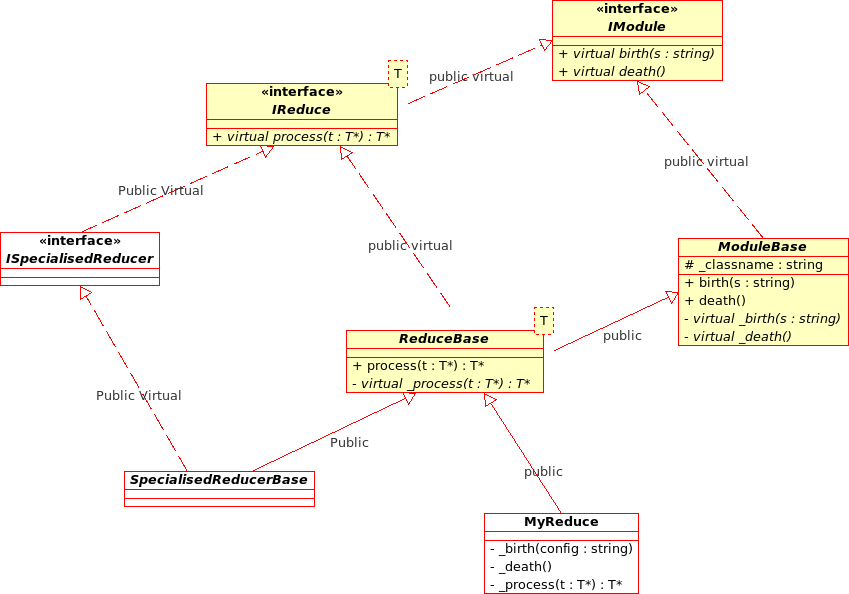
\includegraphics[scale=0.35]{MausApiInheritanceLadder}
  \caption{Inheritance ladder}
\end{figure}

\section{Global Objects - Objects for Many Modules}
There are some objects that sit outside the scope of the modular framework above. Typically these are objects that do not belong to any one module, but need to be accessed by many. Examples are the logging functionality (Squeak), ErrorHandler, Configuration datacards, field maps, geometry description and Geant4 interfaces. These are accessed through the static singleton class \emph{Globals} defined in \emph{src/common_cpp/Utils/Globals.hh}. Initialisation is handled in \emph{src/common_cpp/Globals/GlobalsManager.hh}. One Globals instance is initialised per subprocess when running in multiprocessing mode.



\chapter{Running the Monte Carlo}
\label{chapter:simulation}
The simulation module provides particle generation routines, GEANT4 bindings to track particles through the geometry and routines to convert modelled energy loss in detectors into digitised signals from the MICE DAQ. The Digitisation models are documented under each detector. Here we describe the beam generation and GEANT4 interface.

\section{Beam Generation}
Beam generation is handled by the MapPyBeamMaker module. Beam generation is separated into two classes. The MapPyBeamGenerator has routines to assign particles to a number of individual beam classes, each of which samples particle data from a predefined parent distribution. Beam generation is handled by the \verb|beam| datacard.

The MapPyBeamMaker can either take particles from an external file, overwrite existing particles in the spill, add a specified number of particles from each beam definition, or sample particles from a binomial distribution. The random seed is controlled at the top level and different algorithms can be selected influencing how this is used to generate random seeds on each particle. 

Each beam definition has routines for sampling from a multivariate gaussian distribution or generating ensembles of identical particles (called "pencil" beams here). Additionally it is possible to produce time distributions that are either rectangular or triangular in time to give a simplistic representation of the MICE time distribution.

The beam definition controls are split into four parts. The \verb|reference| branch defines the centroid of the distribution; the \verb|transverse| branch defines the transverse coordinates, $x, y, px, py$; the \verb|longitudinal| branch defines the longitudinal coordinates - time and energy/momentum and the \verb|coupling| branch defines correlations between longitudinal and transverse. Additionally a couple of parameters are available to control random seed generation and relative weighting between different beam definitions.

In transverse, beams are typically sampled from a multivariate gaussian. The Twiss beam ellipse is defined by
\begin{equation}
\mathbf{B_\perp} = m \left(\begin{array}{cccc}
\epsilon_x \beta_x/p   & -\epsilon_x\alpha_x & 0 & 0 \\
-\epsilon_x\alpha_x & \epsilon_x\gamma_x p  & 0 & 0 \\
0 & 0  & \epsilon_y\beta_y/p  & -\epsilon_y\alpha_y \\
0 & 0 & -\epsilon_y\alpha_y & \epsilon_y\gamma_y p \\
\end{array}\right)
\end{equation}
The Penn beam ellipse is defined by,
\begin{equation}
\mathbf{B_\perp} = m\epsilon_\perp \left(\begin{array}{cccc}
\beta_\perp/p   & -\alpha_\perp & 0 & -\mathcal{L}+\beta_\perp B_0/2p \\
-\alpha_\perp & \gamma_\perp p  & \mathcal{L}-\beta_\perp B_0/2p & 0 \\
0 & \mathcal{L}-\beta_\perp B_0/2p  & \beta_\perp/p  & -\alpha_\perp \\
-\mathcal{L}+\beta_\perp B_0/2p & 0 & -\alpha_\perp & \gamma_\perp p \\
\end{array}\right)
\end{equation}
where parameters can be controlled in datacards

\begin{table*}
\begin{center}
\caption{Control parameters pertaining to all beam definitions.}
\begin{tabularx}{\textwidth}{lX}
Name & Meaning \\
\hline
\verb|beam| & dict containing beam definition parameters.\\
\hline
\multicolumn{2}{l}{\emph{The following cards should all be defined within the \verb|beam| dict.}} \\
\hline
\verb|particle_generator| & Set to \verb|binomial| to choose the number of particles by sampling from a binomial distribution. Set to \verb|counter| to choose the number of particles in each beam definition explicitly. Set to \verb|file| to generate particles by reading an input file. Set to \verb|overwrite_existing| to generate particles by overwriting existing primaries. \\
\verb|binomial_n| & When using a binomial \verb|particle_generator|, this controls the number of trials to make. Otherwise ignored. \\
\verb|binomial_p| & When using a binomial \verb|particle_generator|, this controls the probability a trial yields a particle. Otherwise ignored. \\
\verb|beam_file_format| & When using a file \verb|particle_generator|, set the input file format - options are 
                          \begin{itemize}
                            \setlength{\itemsep}{0mm}
                            \item \verb|icool_for009|
                            \item \verb|icool_for003|,
                            \item \verb|g4beamline_bl_track_file|
                            \item \verb|g4mice_special_hit|
                            \item \verb|g4mice_virtual_hit|
                            \item  \verb|mars_1|
                            \item \verb|maus_virtual_hit|
                            \item \verb|maus_primary|
                          \end{itemize}\\
\verb|beam_file|&  When using a file \verb|particle_generator|, set the input file name. Environment variables are automatically expanded by MAUS.\\
\verb|file_particles_per_spill| & When using a file \verb|particle_generator|, this controls the number of particles per spill that will be read from the file.\\
\verb|random_seed| & Set the random seed, which is used to generate individual random seeds for each primary (see below). \\
\verb|definitions| & A list of dicts, each item of which is a dict defining the distribution from which to sample individual particles. \\
\begin{makeimage} % force latex2html to render as an html table 
\end{makeimage} 
\end{tabularx}
\end{center}
\end{table*}


\begin{table*}
\begin{center}
\caption{Individual beam distribution parameters.}
\begin{tabularx}{\linewidth}{lX}
Name & Meaning \\
\hline
\multicolumn{2}{l}{\emph{The following cards should be inside a dict in the beam \verb|definitions| list.}} \\
\hline
\verb|random_seed_algorithm| & Choose from the following options
                          \begin{itemize}
                            \setlength{\itemsep}{0mm}
                            \item \verb|beam_seed|: use the \verb|random_seed| for all particles
                            \item \verb|random|: use a different randomly determined seed for each particle
                            \item \verb|incrementing|: use the \verb|random_seed| but increment by one each time a new particle is generated
                            \item \verb|incrementing_random|: determine a seed at random before any particles are generated; increment this by one each time a new particle is generated
                          \end{itemize}\\
\verb|weight| & When \verb|particle_generator| is \verb|binomial| or \verb|overwrite_existing|, the probability that a particle will be sampled from this distribution is given by $weight/(sumofweights)$.\\
\verb|n_particles_per_spill| & When \verb|particle_generator| is \verb|counter|, this sets the number of particles that will be generated in each spill. \\
\verb|reference| & Dict containing the reference particle definition. \\
\verb|transverse| & Dict defining the longitudinal phase space distribution. \\
\verb|longitudinal| & Dict defining the longitudinal phase space distribution. \\
\verb|coupling| & Dict defining any correlations between transverse and longitudinal. \\
\begin{makeimage} % force latex2html to render as an html table 
\end{makeimage} 
\end{tabularx}
\end{center}
\end{table*}

\begin{table*}
\begin{center}
\caption{Beam distribution reference definition.}
\begin{tabularx}{\linewidth}{lX}
Name & Meaning \\
\hline
\multicolumn{2}{|l|}{\emph{The following cards should be defined in each beam definition \verb|reference| dict.}} \\
\hline
\verb|position| & dict with elements \verb|x|, \verb|y| and \verb|z| that define the reference position (mm).\\
\verb|momentum| & dict with elements \verb|x|, \verb|y| and \verb|z| that define the reference momentum direction. Normalised to 1 at runtime.\\
\verb|particle_id| & PDG particle ID of the reference particle.\\
\verb|energy| & Reference energy. \\
\verb|time| & Reference time (ns). \\
\verb|random_seed| & Set to 0 - this parameter is ignored.\\
\begin{makeimage} 
\end{makeimage} 
\end{tabularx}
\end{center}
\end{table*}

\begin{table*}
\begin{center}
\caption{Beam definition transverse parameters.}
\begin{tabularx}{\linewidth}{lX}
Name & Meaning \\
\hline
\multicolumn{2}{|l|}{\emph{The following cards should be defined in each beam definition \verb|transverse| dict.}} \\
\hline
\verb|transverse_mode| & Options are
                          \begin{itemize}
                            \setlength{\itemsep}{0mm}
                            \item \verb|pencil|: x, py, y, py taken from \verb|reference|
                            \item \verb|penn|: cylindrical beam symmetric in x and y
                            \item \verb|constant_solenoid|: cylindrical beam symmetric in x and y, with beam radius calculated from on-axis B-field to give constant beam radius along a solenoid.
                            \item \verb|twiss|: beam with decoupled x and y beam ellipses.
                          \end{itemize} \\
\hline
\begin{tabular}{l}\verb|normalised_angular_| \\ \verb|momentum| \end{tabular} & if \verb|transverse_mode| is \verb|penn| or \verb|constant_solenoid|, set $\mathcal{L}$.\\
\verb|emittance_4d| & if \verb|transverse_mode| is \verb|penn| or \verb|constant_solenoid|, set $\epsilon_\perp$.\\
\verb|beta_4d| & if \verb|transverse_mode| is \verb|penn|, set $\beta_\perp$.\\
\verb|alpha_4d| & if \verb|transverse_mode| is \verb|penn|, set $\alpha_\perp$.\\
\verb|bz| & if \verb|transverse_mode| is \verb|constant_solenoid|, set the B-field used to calculate $\beta_\perp$ and $\alpha_\perp$.\\
\hline
\verb|beta_x| & if \verb|transverse_mode| is \verb|twiss|, set $\beta_x$.\\
\verb|alpha_x| & if \verb|transverse_mode| is \verb|twiss|, set $\alpha_x$.\\
\verb|emittance_x| & if \verb|transverse_mode| is \verb|twiss|, set $\epsilon_x$.\\
\verb|beta_y| & if \verb|transverse_mode| is \verb|twiss|, set $\beta_y$.\\
\verb|alpha_y| & if \verb|transverse_mode| is \verb|twiss|, set $\alpha_y$.\\
\verb|emittance_y| & if \verb|transverse_mode| is \verb|twiss|, set $\epsilon_y$.\\
\begin{makeimage} % force latex2html to render as an html table 
\end{makeimage} 
\end{tabularx}
\end{center}
\end{table*}


\begin{table*}
\begin{center}
\caption{Beam definition longitudinal parameters.}
\begin{tabularx}{\linewidth}{lX}
Name & Meaning \\
\hline
\multicolumn{2}{l}{\emph{The following cards should be defined in each beam definition \verb|longitudinal| dict.}} \\
\hline
\verb|momentum_variable| & In all modes, set this variable to control which longitudinal variable will be used to control the input beam. Options are \verb|energy|, \verb|p|, \verb|pz|. \\
\verb|longitudinal_mode| & Options are
                          \begin{itemize}
                            \setlength{\itemsep}{0mm}
                            \item \verb|pencil|: time, energy/p/pz taken from \verb|reference|
                            \item \verb|gaussian|: uncorrelated gaussians in time and energy/p/pz
                            \item \verb|twiss|: multivariate gaussian in time and energy/p/pz
                            \item \verb|uniform_time|: gaussian in energy/p/pz and uniform in time.
                            \item \verb|sawtooth_time|: gaussian in energy/p/pz and sawtooth in time.
                          \end{itemize} \\
\hline
\verb|beta_l| & In Twiss mode, set $\beta_l$\\
\verb|alpha_l| & In Twiss mode, set $\alpha_l$\\
\verb|emittance_l| & In Twiss mode, set $\epsilon_l$\\
\hline
\verb|sigma_t| & In \verb|gaussian| mode, set the RMS time. \\
\begin{tabular}{l} \verb|sigma_p| \\ \verb|sigma_energy| \\ \verb|sigma_pz| \end{tabular} & In \verb|gaussian|, \verb|uniform_time|, \verb|sawtooth_time| mode, set the RMS energy/p/pz. \\
\hline
\verb|t_start| & In \verb|uniform_time| and \verb|sawtooth_time| mode, set the start time of the parent distribution \\
\verb|t_end| & In \verb|uniform_time| and \verb|sawtooth_time| mode, set the end time of the parent distribution \\
\begin{makeimage} % force latex2html to render as an html table 
\end{makeimage} 
\end{tabularx}
\end{center}
\end{table*}

\begin{table*}
\begin{center}
\caption{Beam definition coupling parameters.}
\begin{tabularx}{\linewidth}{lX}
Name & Meaning \\
\hline
\multicolumn{2}{l}{\emph{The following cards should be defined in each beam definition \verb|coupling| dict.}} \\
\hline
\verb|coupling_mode| & Set to \verb|none| - not implemented yet. \\
\begin{makeimage} % force latex2html to render as an html table 
\end{makeimage} 
\end{tabularx}
\end{center}
\end{table*}

\section{GEANT4 Bindings}
The GEANT4 bindings are encoded in the Simulation module. GEANT4 groups particles by run, event and track. A GEANT4 run maps to a MICE spill; a GEANT4 event maps to a single inbound particle from the beamline; and a GEANT4 track corresponds to a single particle in the experiment.

A number of classes are provided for basic initialisation of GEANT4.

\begin{itemize}
\item MAUSGeant4Manager: is responsible for handling interface to GEANT4. MAUSGeant4Manager handles initialisation of the GEANT4 bindings as well as accessors for individual GEANT4 objects (see below). Interfaces are provided to run one or many particles through the geometry, returning the relevant event data. The MAUSGeant4Manager sets and clears the event action before each run.
\item MAUSPhysicsList: contains routines to set up the GEANT4 physical processes. Datacards settings are provided to disable stochastic processes or all processes and set a few parameters.
\item FieldPhaser: the field phaser is a MAUS-specific tool for automatically phasing fields, for example RF cavities, such that they ramp coincidentally with incoming particles. The FieldPhaser contains routines to fire test ("reference") particles through the accelerator lattice and phase fields appropriately. The FieldPhaser phasing routines are called after GEANT4 is first initialised.
\item VirtualPlanes: the VirtualPlanes routines are designed to extract particle data from the GEANT4 tracking independently of the GEANT4 geometry. The VirtualPlanes routines watches for steps that step across some plane in physical space, or some time, or some proper time, and then interpolates from the step ends to the plane in question.
\item FillMaterials: (legacy) the FillMaterials routines are used to initialise a number of specific 
\item MICEDetectorConstruction: (legacy) the MICEDetectorConstruction routines provide an interface between the MAUS internal geometry representation encoded in MiceModules and GEANT4. MICEDetectorConstruction is responsible for calling the relevant routines for setting up the general engineering geometry, calling detector-specific geometry set-up routines and calling the field map set-up routines.
\item MAUSVisManager the MAUSVisManager is responsible for handling interfaces with the GEANT4 visualisation.
\end{itemize}

The GEANT4 \emph{Action} objects provide interfaces for MAUS-specific function calls at certain points in the tracking.

\begin{itemize}
\item MAUSRunAction: sets up the running for a particular spill. In MAUS, it just reinitialises the visualisation.
\item MAUSEventAction: sets up the running for a particular inbound particle. At the beginning of each event, the virtual planes, tracking, detectors and stepping are all cleared. After the event the event data is pulled into the event data from each element.
\item MAUSTrackingAction: is called when a new track is created or destroyed. If \verb|keep_tracks| datacard is set to True, on particle creation, MAUSTrackingAction writes the initial and final track position and momentum to the output data tree. If \verb|keep_steps| is set to True MAUSTrackingAction gets step data from MAUSSteppingAction and writes this also.
\item MAUSSteppingAction: is called at each step of the particle. If \verb|keep_steps| datacard is set to True, output step data is recorded. MAUSSteppingAction kills particles if they exceed the \verb|maximum_number_of_steps| datacard. MAUSSteppingAction calls the VirtualPlanes routines on each step.
\item MAUSPrimaryGeneratorAction: is called at the start of every event and sets the particle data for each event. In MAUS, this particle generation is handled externally and so the MAUSPrimaryGeneratorAction role is to look for the primary object on the Monte Carlo event and convert this into a GEANT4 event object.
\item MAUSStackingActionKillNonMuons: is never initialised and should be removed.
\end{itemize}

\begin{table*}
\begin{center}
\caption{Monte Carlo control parameters.}
\begin{tabularx}{\textwidth}{lX}
Name & Meaning \\
\hline
\multicolumn{2}{l}{\emph{General Monte Carlo controls.}} \\
\hline
\verb|simulation_geometry_filename| & Filename for the simulation geometry - searches first in files tagged by environment variable \verb|${MICEFILES}|, then in the local directory.\\
\verb|simulation_reference_particle| & Reference particle used for phasing fields.\\
\verb|keep_tracks| & Set to boolean true to store the initial and final position/momentum of each track generated by MAUS.\\
\verb|keep_steps| & Set to boolean true to store every step generated by MAUS - warning this can lead to large output files.\\
\verb|maximum_number_of_steps| & Set to an integer value. Tracks taking more steps are assumed to be looping.\\
\begin{makeimage} % force latex2html to render as an html table 
\end{makeimage} 
\end{tabularx}
\end{center}
\end{table*}

\begin{table*}
\begin{center}
\caption{Physics list control parameters.}
\begin{tabularx}{\textwidth}{lX}
\hline
\multicolumn{2}{l}{\emph{Physics list controls.}} \\
\hline
\verb|physics_model| & GEANT4 physics model used to set up the physics list.\\
\verb|physics_processes| & Choose which physics processes normal particles observe during tracking. Options are 
                            \begin{itemize}
                            \item \verb|normal| particles will obey normal physics processes, scattering and energy straggling will be active.
                            \item \verb|mean_energy_loss| particles will lose a deterministic amount of energy during interaction with materials and will never decay.
                            \item \verb|none| Particles will never lose energy or scatter during tracking and will never decay.
                            \end{itemize} \\
\verb|reference_physics_processes| & Choose which physics processes the reference particle observes during tracking. Options are \verb|mean_energy_loss| and \verb|none|. The reference particle can never have stochastic processes enabled.\\
\verb|particle_decay| & Set to boolean true to enable particle decay; set to boolean false to disable.\\
\verb|charged_pion_half_life| & Set the half life for charged pions.\\
\verb|muon_half_life| & Set the half life for muons.\\
\verb|production_threshold| & Set the geant4 production threshold.\\
\begin{makeimage} % force latex2html to render as an html table 
\end{makeimage} 
\end{tabularx}
\end{center}
\end{table*}

\begin{table*}
\begin{center}
\caption{Visualisation control parameters.}
\begin{tabularx}{\textwidth}{lX}
\hline
\multicolumn{2}{l}{\emph{Visualisation controls.}} \\
\hline
\verb|geant4_visualisation| & Set to boolean true to activate GEANT4 visualisation.\\
\verb|visualisation_viewer| & Control which viewer to use to visualise GEANT4 tracks. Currently only vrmlviewer is compiled into GEANT4 by default. Users can recompile GEANT4 with additional viewers enabled at their own risk.\\
\verb|visualisation_theta| & Set the theta angle of the camera.\\
\verb|visualisation_phi| & Set the phi angle of the camera.\\
\verb|visualisation_zoom| & Set the camera zoom.\\
\verb|accumulate_tracks| & Set to 1 to accumulate all of the simulated tracks into one vrml file. 0 for multiple files.\\
\verb|default_vis_colour| & Set the RGB values to alter the default colour of particles.\\
\verb|pi_plus_vis_colour| & Set the RGB values to alter the colour of positive pions.\\
\verb|pi_minus_vis_colour| & Set the RGB values to alter the colour of negative pions.\\
\verb|mu_plus_vis_colour| & Set the RGB values to alter the colour of positive muons.\\
\verb|mu_minus_vis_colour| & Set the RGB values to alter the colour of negative pions.\\
\verb|e_plus_vis_colour| & Set the RGB values to alter the colour of positrons.\\
\verb|e_minus_vis_colour| & Set the RGB values to alter the colour of electrons.\\
\verb|gamma_vis_colour| & Set the RGB values to alter the colour of gammas.\\
\verb|neutron_vis_colour| & Set the RGB values to alter the colour of neutrons.\\
\verb|photon_vis_colour| & Set the RGB values to alter the colour of photons.\\
\begin{makeimage} % force latex2html to render as an html table 
\end{makeimage} 
\end{tabularx}
\end{center}
\end{table*}



MAUS uses the online Configuration Database to store all of its geometries. These geometries have been transferred from CAD drawings which are
modelling using the latest surveys and technical drawings available. The following section shall describe how to use the available executables to
access and use these models. 

\section{Geometry Download}

There are two executable files available to users both can be found in the directory /bin/utilities found within your copy of MAUS. The two files of
interest are download\_geometry.py and get\_geometry\_ids.py. These files do the following.

\begin{description}
  \item[Upload Geometry] \hfill 
  \begin{enumerate}
   \item Set up the Configreader class and read the values provided by ConfigurationDefaults.py or by custom config files.
   \item Instantiate an Uploader class object using the upload directory and geometry note taken from the configuration file.
   \item The list of files which is created by the Uploader class is used to compress the geometry files into one zip file.
   \item This zip file is then used as the argument for the upload\_to\_CDB method which takes the contents of the zip and then uploads this, as a
single string to the CDB.
   \item[Optional] If cleanup is specified in the configuration file then the file list and the original GDML files are the deleted leaving only the
zip file.
  \end{enumerate}

  \item[Download Geometry] \hfill
  \begin{enumerate}
   \item Set up the Configreader() class and read the values provided by ConfigurationDefaults.py or by custom config files.
   \item Instantiate a Downloader class object and downloads either the current, time specified or run number zipped geometry to a temporary cache
location.
   \item The zip file is then unzipped in this location.
   \item The Formatter class is then called and this class formats the GDMLs. The formatting alters the schema location of these files and points
them to the correct local locations of the Materials GDML file. This formatting leaves the original GDMLs in the tmeporary cache and places the new
formatted files in the download directory specified in the configuration file.
   \item GDMLtoMAUS is then called with the location of the new formatted files as its argument. This class converts the GDMLs to the MICE Module
text files using the XSLT stylesheets previously described.
   \item[Optional] If specified in the configuration file the temporary cache location is removed along with the zip file and unzipped files.
  \end{enumerate}

  \item[Get Geometry IDs]
  \begin{enumerate}
   \item Set up the Configreader() class and read the values provided by ConfigurationDefaults.py or by custom config files. This file takes start
and stop time arguments to specify a period to search the CDB.
   \item A CDB class object is then instantiated with the server specified in the configuration file.
   \item The get ids method from the CDB class is called and the python dict which is downloaded is formatted and either printed to screen or to file
as specified in the configuration file.
  \end{enumerate}
\end{description}

To use these files the user must use the arguments in the ConfigurationDefaults.py file. The arguments relating to these executables are as follows.

\begin{table*}
\begin{center}
\caption{Geometry control parameters.}
\begin{tabularx}{\textwidth}{lX}
\hline
\multicolumn{2}{l}{\emph{Geometry controls.}} \\
\hline
\verb|cdb_upload_url| & Sets the upload url relating the the Configuration Database.\\
\verb|cdb_download_url| & Sets the download url relating the the Configuration Database.\\
\verb|geometry_download_wsdl| & Name of the web service used for downloads.\\
\verb|geometry_download_directory| & Set the directory where you wish the geometry to be downloaded to.\\
\verb|geometry_download_by| & This can be set to either \textit{current, id or run\_number}. Current will download the current valid geometry stored
on the CDB. ID will download the geometry for the ID specified N.B ID numbers can be found using the get geometry ids executable. Run\_number will
download the geometry along with control room information for specified run. \\ 
\verb|geometry_download_run_number| & Set the number of the run to be downloaded.\\
\verb|geometry_download_id| & Set the number of the geometry ID to be downloaded.\\
\verb|geometry_download_cleanup| & Set to True in order to cleanup the temporary files creaated during the download process. These are the zip file
downloaded and the original GDML files from this zip file.\\
\verb|g4_step_max| & Set the G4 step max number which will be set in the ParentGeometryFile. This relates to the size of steps carried out during
the simulation.\\
\verb|geometry_upload_wsdl| & Name of the web service used for uploads. For developers use only.\\
\verb|geometry_upload_directory| & Set the the directory which stores the FastRad produced GDML files which will be stored on the CDB. For Developers
use only.\\
\verb|geometry_upload_note| & Write the description of the geometry which is going to be uploaded. This should describe what is in the beam line
specifically what is new to the model. It should also include any other information the developer wishes the user to know. For developers use only.\\
\verb|geometry_upload_valid_from| & Set the date-time format of the date when this geometry about to be uploaded is valid from. For developers use
only.\\
\verb|geometry_upload_cleanup| & Set to True in order to cleanup the temporary files creaated during the upload process. These are the file
containing the list of GDMLs to be uploaded and also the original GDML files. For developers use only.\\
\verb|get_ids_start_time| & Set the start time of the period which you would like to get the ids from the configuration database. Must be in
date-time format.\\
\verb|get_ids_stop_time| & Set the stop time of the period which you would like to get the ids from the configuration database. Must be in
date-time format.\\
\verb|get_ids_create_file| & Set to True in order to create a file which lists the geometries available within the time period specified. If set to
False the geometry information will be printed to screen.\\
\begin{makeimage} % force latex2html to render as an html table 
\end{makeimage} 
\end{tabularx}
\end{center}
\end{table*}


% mice modules documentation originally from open office - hence some weirdness
% historical MiceModule.pdf document in doc/doc_src/run_control
%\newcommand\textsubscript[1]{\ensuremath{{}_{\text{#1}}}}
% Outline numbering
%\setcounter{secnumdepth}{0}
\makeatletter
\newcommand\arraybslash{\let\\\@arraycr}
\makeatother
% List styles
\newcommand\liststyleLi{%
\renewcommand\labelitemi{${\bullet}$}
\renewcommand\labelitemii{${\circ}$}
\renewcommand\labelitemiii{${\blacksquare}$}
\renewcommand\labelitemiv{${\bullet}$}
}
\newcommand\liststyleLii{%
\renewcommand\labelitemi{${\bullet}$}
\renewcommand\labelitemii{${\circ}$}
\renewcommand\labelitemiii{${\blacksquare}$}
\renewcommand\labelitemiv{${\bullet}$}
}
\newcommand\liststyleLiii{%
\renewcommand\labelitemi{${\bullet}$}
\renewcommand\labelitemii{${\circ}$}
\renewcommand\labelitemiii{${\blacksquare}$}
\renewcommand\labelitemiv{${\bullet}$}
}
\newcommand\liststyleLiv{%
\renewcommand\labelitemi{${\bullet}$}
\renewcommand\labelitemii{${\circ}$}
\renewcommand\labelitemiii{${\blacksquare}$}
\renewcommand\labelitemiv{${\bullet}$}
}
\newcommand\liststyleLv{%
\renewcommand\labelitemi{${\bullet}$}
\renewcommand\labelitemii{${\circ}$}
\renewcommand\labelitemiii{${\blacksquare}$}
\renewcommand\labelitemiv{${\bullet}$}
}
\newcommand\liststyleLvi{%
\renewcommand\labelitemi{${\bullet}$}
\renewcommand\labelitemii{${\circ}$}
\renewcommand\labelitemiii{${\blacksquare}$}
\renewcommand\labelitemiv{${\bullet}$}
}
\newcommand\liststyleLvii{%
\renewcommand\labelitemi{${\bullet}$}
\renewcommand\labelitemii{${\circ}$}
\renewcommand\labelitemiii{${\blacksquare}$}
\renewcommand\labelitemiv{${\bullet}$}
}
\newcommand\liststyleLviii{%
\renewcommand\labelitemi{{\textbullet}}
\renewcommand\labelitemii{${\circ}$}
\renewcommand\labelitemiii{${\blacksquare}$}
\renewcommand\labelitemiv{{\textbullet}}
}
\newcommand\liststyleLix{%
\renewcommand\labelitemi{{\textbullet}}
\renewcommand\labelitemii{${\circ}$}
\renewcommand\labelitemiii{${\blacksquare}$}
\renewcommand\labelitemiv{{\textbullet}}
}
\newcommand\liststyleLx{%
\renewcommand\labelitemi{{\textbullet}}
\renewcommand\labelitemii{${\circ}$}
\renewcommand\labelitemiii{${\blacksquare}$}
\renewcommand\labelitemiv{{\textbullet}}
}
\newcommand\liststyleLxi{%
\renewcommand\theenumi{\arabic{enumi}}
\renewcommand\theenumii{\arabic{enumii}}
\renewcommand\theenumiii{\arabic{enumiii}}
\renewcommand\theenumiv{\arabic{enumiv}}
\renewcommand\labelenumi{\theenumi.}
\renewcommand\labelenumii{\theenumii.}
\renewcommand\labelenumiii{\theenumiii.}
\renewcommand\labelenumiv{\theenumiv.}
}
\newcommand\liststyleLxii{%
\renewcommand\labelitemi{${\bullet}$}
\renewcommand\labelitemii{${\circ}$}
\renewcommand\labelitemiii{${\blacksquare}$}
\renewcommand\labelitemiv{${\bullet}$}
}
\newcommand\liststyleLxiii{%
\renewcommand\labelitemi{${\bullet}$}
\renewcommand\labelitemii{${\circ}$}
\renewcommand\labelitemiii{${\blacksquare}$}
\renewcommand\labelitemiv{${\bullet}$}
}
\newcommand\liststyleLxiv{%
\renewcommand\labelitemi{${\bullet}$}
\renewcommand\labelitemii{${\circ}$}
\renewcommand\labelitemiii{${\blacksquare}$}
\renewcommand\labelitemiv{${\bullet}$}
}
% Page layout (geometry)
\setlength\voffset{-1in}
\setlength\hoffset{-1in}
\setlength\topmargin{2cm}
\setlength\oddsidemargin{2cm}
\setlength\textheight{23.017668cm}
\setlength\textwidth{17.59cm}
\setlength\footskip{26.144882pt}
\setlength\headheight{0cm}
\setlength\headsep{0cm}
% Footnote rule
\setlength{\skip\footins}{0.119cm}
\renewcommand\footnoterule{\vspace*{-0.018cm}\setlength\leftskip{0pt}\setlength\rightskip{0pt plus 1fil}\noindent\textcolor{black}{\rule{0.25\columnwidth}{0.018cm}}\vspace*{0.101cm}}
% Pages styles
\makeatletter
\newcommand\ps@Standard{
  \renewcommand\@oddhead{}
  \renewcommand\@evenhead{}
  \renewcommand\@oddfoot{\thepage{}}
  \renewcommand\@evenfoot{\@oddfoot}
  \renewcommand\thepage{\arabic{page}}
}

 % just some definitions for latex
\chapter{How to Define a Geometry}
Mice Modules are the objects that control the geometry and fields that are simulated in MAUS. They are used in
conjunction with a datacard file, which provides global run control parameters. Mice Modules are created by reading in
a series of text files when MAUS applications are run.

This geometry information is used primarily by the Simulation application for tracking of particles through magnetic
fields. A few commands are specific to detector Reconstruction and accelerator beam Optics applications.

The Mice Modules are created in a tree structure. Each module is a parent of any number of child modules. Typically the
parent module will describe a physical volume, and child modules will describe physical volumes that sit inside the
parent module. Modules cannot be used to describe volumes that do not sit at least partially inside the volume if the
parent module.

Each Mice Module file consists of a series of lines of text. Firstly the Module name is defined. This is followed by an
opening curly bracket, then the description of the module and the placement of any child modules, and finally a closing
curly bracket. Commands, curly brackets etc must be separated by an end of line character.

Comments are indicated using either two slashes or an exclamation mark. Characters placed after a comment on a line are
ignored.

MAUS operates in a right handed coordinate system $(x,y,z)$. In the absence of any rotation, lengths are
considered to be extent along the \textit{z}{}-axis, widths to be extent along the \textit{x}{}-axis and heights to be
extent along the \textit{y}{}-axis. Rotations $(\theta_{x}, \theta_{y}, \theta_{z})$ are defined
as a rotation about the z-axis through $\theta_{z}$, followed by a rotation about the y-axis through
$\theta_{y}$, followed by a rotation about the x-axis through $\theta_{x}$.

\subsection{Configuration File}
The Configuration file places the top level objects in MICE. The location of the file is controlled by the datacard
\verb|simulation_geometry_file_name|. MAUS looks for the configuration file in the first instance in the directory
\begin{verbatim}
    ${MICEFILES}/Models/Configuration/<MiceModel>
\end{verbatim}
where \verb|${MICEFILES}| is a user-defined environment variable. If MAUS fails to find the file it searches the
local directory.

The world volume is defined in the Configuration file and any children of the world volume are referenced by the
Configuration file. The Configuration file looks like

\begin{verbatim}
    Configuration <Configuration Name>
    {
        Dimensions <x> <y> <z> <Units>
        <Properties>
        <Child Modules>
    }
\end{verbatim}

\verb|<Configuration Name>| is the name of the configuration. Typically the Configuration file
name is given by \verb|<Configuration Name>.dat|. The world volume is always a rectangular box
centred on $(0,0,0)$ with $x$, $y$, and $z$ extent set by the Dimensions. Properties and Child Modules are described below and
added as in any Module.

\subsubsection{Substitutions}
It is possible to make keyword substitutions that substitutes all instances of \verb|<name>| with
\verb|<value>| in all Modules. The syntax is

\begin{verbatim}
    Substitution <name> <value>
\end{verbatim}

\verb|<name>| must start with a single \$ sign. Substitutions must be defined in the Configuration file.
Note this is a direct text substitution in the MiceModules before the modules are parsed properly. So for example,

\begin{verbatim}
    Substitution $Sub SomeText
    PropertyString FieldType \$Sub}
    PropertyDouble \$SubValue 10}
\end{verbatim}

would be parsed as MAUS like

\begin{verbatim}
    PropertyString FieldType SomeText}
    PropertyDouble SomeTextValue 10}
\end{verbatim}

\subsubsection{Expressions}
The use of equations in properties of type double and Hep3Vector is also allowed in place of a single value. So, for
example, 
\begin{verbatim}
    PropertyDouble FieldStrength 0.5*2 T
\end{verbatim}
would result in a FieldStrength property of 1 Tesla.\texttt{ }

\subsubsection{Expression Substitutions}
Some additional variables can be defined in specific cases by MAUS itself for substitution into experssions, in which
case they will start with @ symbol. For these variable substitutions, it is only possible to make the substitution into
expressions. So for example,
\begin{verbatim}
    PropertyDouble ScaleFactor 2*@RepeatNumber
\end{verbatim}
Would substitute @RepeatNumber \ into the expression. @RepeatNumber \ is defined by MAUS when repeating modules are
used (see RepeatModule2, below). Note the following code is not valid
\begin{verbatim}
    PropertyString FileName File@RepeatNumber //NOT VALID
\end{verbatim}
This is because Expression Substitutions can only be used in an expression (i.e. an equation).

\subsection[Module Files]{Module Files}
Children of the top level Mice Module are defined by Modules. MAUS will attempt to find a module in an external file.
The location of the file is controlled by the parent Module. Initially MAUS looks in the directory
\begin{verbatim}
    ${MICEFILES}/Models/Modules/<Module>
\end{verbatim}
If the Mice Module cannot be found, MAUS searches the local directory. If the module file still cannot be found,
MAUS will issue a warning and proceed.

The Module description is similar in structure to the Configuration file:
\begin{verbatim}
    Module <Module Name>
    {
        Volume  <Volume Type>
        Dimensions  <Dimension1> <Dimension2> <Dimension3> <Units>
        <Properties>

        <Child Modules>
    }
\end{verbatim}
\verb|<Module Name>| is the name of the module. Typically the Module file name is given by
\verb|<Module Name>.dat|.

The definition of Volume, Dimensions, Properties and Child Modules are described below.

\subsection{Volume and Dimensions}
The volume described by the MiceModule can be one of several types. Replace \verb|<Volume Type>| with the
appropriate volume below. Cylinder, Box and Tube define cylindrical and cuboidal volumes.
Polycone defines an arbitrary volume of rotation and is described in detail below. Wedge describes a wedge with a
triangular projection in the y-z plane and rectangular projections in x-z and x-y planes. Quadrupole defines an
aperture with four cylindrical pole tips.

In general, the physical volumes that scrape the beam are defined independently of the field maps. This is the more
versatile way to do things, but there are some pitfalls which such an implementation introduces. For example, in
hard-edged fields like pillboxes, tracking errors can be introduced when MAUS steps into the field region. This can
be avoided by adding windows (probably made of vacuum material) to force GEANT4 to stop tracking, make a small step
over the field boundary, and then restart tracking inside the field. However, such details are left for the user to
implement.

\begin{center}
\tablefirsthead{\hline
{\bfseries Volume} &
\multicolumn{1}{m{4.321cm}|}{{\bfseries Dimension1}} &
\multicolumn{1}{m{4.564cm}|}{{\bfseries Dimension2}} &
{\bfseries Dimension3}\\}
\tablehead{\hline
{\bfseries Volume} &
\multicolumn{1}{m{4.321cm}|}{{\bfseries Dimension1}} &
\multicolumn{1}{m{4.564cm}|}{{\bfseries Dimension2}} &
{\bfseries Dimension3}\\}
\tabletail{}
\tablelasttail{}
\begin{supertabular}{|m{2.659cm}|m{4.321cm}m{4.564cm}m{5.25cm}|}
\hline
None &
\multicolumn{3}{m{14.535cm}|}{No dimensions required. Note cannot define daughter Modules for this volume type.}\\\hline
Cylinder &
\multicolumn{1}{m{4.321cm}|}{Radius} &
\multicolumn{1}{m{4.564cm}|}{Length in z} &
Not used (leave blank)\\\hline
Box &
\multicolumn{1}{m{4.321cm}|}{Width in x} &
\multicolumn{1}{m{4.564cm}|}{Height in y} &
Length along z\\\hline
Tube &
\multicolumn{1}{m{4.321cm}|}{Inner Radius} &
\multicolumn{1}{m{4.564cm}|}{Outer Radius} &
Length in z\\\hline
Trapezoid &
\multicolumn{1}{m{4.321cm}|}{Half Width in x} &
\multicolumn{1}{m{4.564cm}|}{Half Height in y} &
Half Length in z\\\hline
Wedge &
\multicolumn{3}{m{14.535cm}|}{See documentation below.}\\\hline
Polycone &
\multicolumn{3}{m{14.535cm}|}{No dimensions required. Volume defined from external file.}\\\hline
Quadrupole &
\multicolumn{3}{m{14.535cm}|}{No dimensions required. Dimensions defined from module properties.}\\\hline
Multipole &
\multicolumn{3}{m{14.535cm}|}{No dimensions required. Dimensions defined from module properties.}\\\hline
Boolean &
\multicolumn{3}{m{14.535cm}|}{No dimensions required. Dimensions defined from module properties.}\\\hline
Sphere &
\multicolumn{3}{m{14.535cm}|}{See documentation below.}\\\hline
\end{supertabular}
\end{center}

\subsection{Properties}
Many of the features of MAUS that can be enabled in a module are described using properties. For example, properties
enable the user to define detectors and fields. Properties can be either of several types: PropertyDouble,
PropertyString, PropertyBool, PropertyHep3Vector or PropertyInt. A property is declared via
\begin{verbatim}
    <Property Type> <Property Name> <Value> <Units if appropriate>
\end{verbatim}
Different properties that can be enabled for Mice Modules are described elsewhere in this document. Properties of type
PropertyDouble and PropertyHep3Vector can have units. Units are defined in the CLHEP library. Units are case sensitive;
MAUS will return an error message if it fails to parse units. Combinations of units such as T/m or N*m can be defined
using '*' and '/' as appropriate. Properties cannot be defined more than once within the same module.

\subsection{Child Modules}
Child Modules are defined with a position, rotation and scale factor. This places, and rotates, the child volume and any
fields present relative to the parent volume. Scale factor scales fields defined in the child module and any of its
children. Scale factors are recursively multiplicative; that is the field generated by a child module will be scaled by
the product of the scale factor defined in the parent module and all of its parents.

The child module definition looks like:
\begin{verbatim}
    Module <Module File Name>
    {
        Position  <x position> <y position> <z position> <Units>
        Rotation  <x rotation> <y rotation> <z rotation> <Units>
        ScaleFactor <Value>
        <Define volume, dimensions and properties for this instance only>
    }
\end{verbatim}
MAUS searches for \verb|<Module File Name>| first relative to \verb|${MICEFILES}/Models/Modules/| and subsequently
relative to the current working directory. The position and rotation default to $0, 0, 0$ and the \verb|scale factor| defaults
to $1$.

\liststyleLi
\begin{itemize}
\item Volume, Dimension and Properties of the child module can be defined at the level of the parent; in this case these
values will be used only for this instance of the module.
\end{itemize}
\liststyleLii
\begin{itemize}
\item If no file can be found, MAUS will press on regardless, attempting to build a geometry using the information
defined in the parent volume.
\end{itemize}
\subsection[Module Hierarchy and GEANT4 Physical Volumes]{Module Hierarchy and GEANT4 Physical Volumes}
\begin{figure}[!htb]
\begin{center}
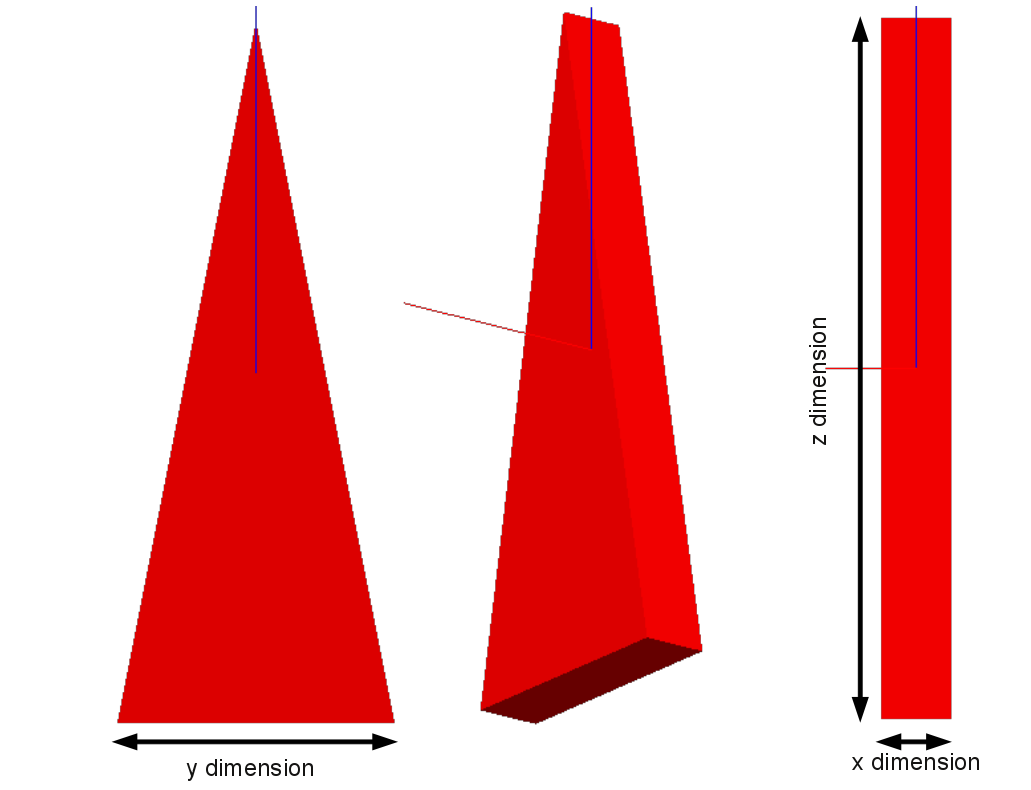
\includegraphics[width=0.5\textwidth]{mice_modules/volume_hierarchy.png}
\caption{The diagram shows a schematic for a square placed inside a cylinder inside a rectangle. This nesting must be replicated
         in the MiceModules in order for the volumes to be correctly represented by MAUS.}
\end{center}
\end{figure}
MAUS enables users to place arbitrary physical volumes in a GEANT4 geometry. The
formatting of MAUS is such that users are encouraged to use the GEANT4 tree structure for placing physical volumes.
This is a double-edged sword, in that it provides users with a convenient interface for building geometries, but it is
not a terribly safe interface.

Consider the cartoon of physical volumes shown above. Here there is a blue volume sitting inside a red volume sitting
inside the black world volume. For the volumes to be represented properly, the module that represents the blue volume
MUST be a child of the module that represents the red volume. The module that represents the red volume MUST, in turn,
be a child of the module that represents the black volume, in this case the Configuration file.

What would happen if we placed the blue volume directly into the Black volume, i.e. the Configuration file? GEANT4 would
silently ignore the blue volume, or the red volume, depending on the order in which they are added into the GEANT4
geometry. What would happen if we placed the blue volume overlapping the red and black volumes? The behaviour of GEANT4
is not clear in this case.

\liststyleLiii
\begin{itemize}
\item Never allow a volume to overlap any part of another volume that is not it's direct parent.
\end{itemize}
It is possible to check for overlaps by setting the datacard \textit{CheckVolumeOverlaps} to 1.

\subsection{A Sample Configuration File}
Below is listed a sample configuration file, which is likely to be included in the file
\textit{ExampleConfiguration.dat;} the actual name is specified by the datacard MiceModel.
\begin{verbatim}
    Configuration ExampleConfiguration
    {
        Dimensions 1500.0 1000.0 5000.0 cm
        PropertyString Material AIR
        Substitution $MyRedColour 0.75
        Module BeamLine/SolMag.dat
        {
            Position 140.0 0.0 -2175.0 cm
            Rotation 0.0 30.0 0.0 degree
            ScaleFactor 1.
        }
        Module BeamLine/BendMag.dat
        {
            Position 0.0 0.0 -1935.0 cm
            Rotation 0.0 15.0 0.0 degree
            ScaleFactor 1.
        }
        Module NoFile_Box1
        {
            Volume Box
            Dimension 1.0 1.0 1.0
            Position 0.0 0.0 200.0 cm
            Rotation 0.0 15.0 0.0 degree
            PropertyString Material  Galactic
            PropertyDouble RedColour $MyRedColour
        }
        Module NoFile_Box2}
        {
            Volume Box
            Dimension 0.5 0.5 0.5*3 m //z length = 0.5*3 = 1.5 m
            Rotation  0.0 15.0 0.0 degree //Rotation relative to parent
            PropertyString Material  Galactic
            PropertyDouble RedColour $MyRedColour
        }
    }
\end{verbatim}

\subsection{A Sample Child Module File}
Below is listed a sample module file, which is likely to be included in the file \textit{SolMag.dat}; the actual
location is specified by the module or configuration that calls FCoil. The module contains a number of properties that
define the field.

\begin{verbatim}
    Module SolMag
    {
        Volume Tube
        Dimensions 263.0 347.0 210.0 mm
        PropertyString Material Al
        PropertyDouble BlueColour 0.75
        PropertyDouble GreenColour 0.75
        //field}
        PropertyString FieldType      Solenoid
        PropertyString FileName       focus.dat
        PropertyDouble CurrentDensity 1.
        PropertyDouble Length         210. mm
        PropertyDouble Thickness      84. mm
        PropertyDouble InnerRadius    263. mm
    }
\end{verbatim}

 % how to use mice modules
\chapter{Geometry and Tracking MiceModule Properties}
In general, MAUS treats physical geometry distinct from fields. Fields can be placed overlapping physical
objects, or entirely independently of them, as the user desires. Properties for various aspects of the
physical and engineering model of the simulation are described below. This includes properties for
sensitive detectors.

\subsection{General Properties}
There are a number of properties that are applicable to any MiceModule.

\begin{center}
\tablefirsthead{\hline
{\bfseries Property} &
{\bfseries Type} &
{\bfseries Description}\\}
\tablehead{\hline
{\bfseries Property} &
{\bfseries Type} &
{\bfseries Description}\\}
\tabletail{}
\tablelasttail{}
\begin{supertabular}{|m{3.665cm}|m{1.278cm}|m{12.052cm}|}
\hline
Material &
string &
The material that the volume is made up from\\\hline
Invisible &
bool &
Set to 1 to make the object invisible in visualisation, or 0 to make the object visible.\\\hline
\multicolumn{2}{m{5.143cm}|}{\hspace*{-\tabcolsep}\begin{tabular}{|m{3.665cm}|m{1.278cm}}

RedColour &
double\\\hline
GreenColour &
double\\\hline
BlueColour &
double\\\hline
\end{tabular}\hspace*{-\tabcolsep}
} &
Alter the colour of objects as they are visualised\\\hhline{~~-}
G4StepMax &
double &
The maximum step length that Geant4 can make in the volume. Inherits values from the parent volumes.\\\hline
\multicolumn{2}{m{5.143cm}|}{\hspace*{-\tabcolsep}\begin{tabular}{|m{3.665cm}|m{1.278cm}}

G4TrackMax &
double\\\hline
G4TimeMax &
double\\\hline
\end{tabular}\hspace*{-\tabcolsep}
} &
The maximum track length and particle time of a track. Tracks outside this bound are killed. Inherits values from the
parent volumes.\\\hhline{~~-}
G4KinMin &
double &
The minimum kinetic energy of a track. Tracks outside this bound are killed. Inherits values from the parent
volumes.\\\hline
SensitiveDetector &
string &
Set to the type of sensitive detector required. Possible sensitive detectors are \textit{TOF}, \textit{SciFi},
\textit{CKOV}, \textit{SpecialVirtual, Virtual, Envelope} or \textit{EMCAL}.\\\hline
\end{supertabular}
\end{center}
\subsection{Sensitive Detectors}
A sensitive detector (one in which hits are recorded) can be defined by including the SensitiveDetector property. When a
volume is set to be a sensitive detector MAUS will automatically record tracks entering, exiting and crossing the
volume. Details such as the energy deposited by the track are sometimes also recorded in order to enable subsequent
modelling of the detector response.

Some sensitive detectors use extra properties.

\subsubsection[Scintillating Fibre Detector (SciFi)]{Scintillating Fibre Detector (SciFi)}
\subsubsection{Cerenkov Detector (CKOV)}
\subsubsection{Time Of Flight Counter (TOF)}
\subsubsection{Special Virtual Detectors}
Special virtual detectors are used to monitor tracking through a particular physical volume. Normally particle tracks
are written in the global coordinate system, although an alternate coordinate system can be defined. Additional
properties can be used to parameterise special virtual detectors.

\begin{center}
\tablefirsthead{\hline
{\bfseries Property} &
{\bfseries Type} &
{\bfseries Description}\\}
\tablehead{\hline
{\bfseries Property} &
{\bfseries Type} &
{\bfseries Description}\\}
\tabletail{}
\tablelasttail{}
\begin{supertabular}{|m{3.665cm}|m{1.3579999cm}|m{11.973001cm}|}
\hline
\multicolumn{2}{m{5.223cm}|}{\hspace*{-\tabcolsep}\begin{tabular}{|m{3.665cm}|m{1.3579999cm}}

ZSegmentation &
int\\\hline
PhiSegmentation &
int\\\hline
RSegmentation &
int\\\hline
\end{tabular}\hspace*{-\tabcolsep}
} &
Set the number of segments in the detector in Z, R or f. Defaults to 1.\\\hhline{~~-}
\multicolumn{2}{m{5.223cm}|}{\hspace*{-\tabcolsep}\begin{tabular}{|m{3.665cm}|m{1.3579999cm}}

SteppingThrough &
bool\\\hline
SteppingInto &
bool\\\hline
SteppingOutOf &
bool\\\hline
SteppingAcross &
bool\\\hline
\end{tabular}\hspace*{-\tabcolsep}
} &
Set to true to record tracks stepping through, into, out of or across the volume. Defaults to true.\\\hhline{~~-}
Station &
int &
Define an integer that is written to the output file to identify the station. Defaults to a unique integer identifier
chosen by MAUS, which will be different each time the same Special Virtual is placed.\\\hline
LocalRefRotation &
Hep3

Vector &
If set, record hits relative to a reference rotation in the coordinate system of the SpecialVirtual detector.\\\hline
GlobalRefRotation &
Hep3

Vector &
If set, record hits relative to a reference rotation in the coordinate system of the Configuration.\\\hline
LocalRefPosition &
Hep3

Vector &
If set, record hits relative to a reference position in the coordinate system of the SpecialVirtual detector.\\\hline
GlobalRefPosition &
Hep3

Vector &
If set, record hits relative to a reference position in the coordinate system of the Configuration.\\\hline
\end{supertabular}
\end{center}
\subsubsection{Virtual Detectors}
Virtual detectors are used to extract all particle data at a particular plane, irrespective of geometry. Virtual
detectors do not need to have a physical volume. The \textit{plane} can be a plane in z, time, proper time, or a
physical plane with some arbitrary rotation and translation.

\begin{center}
\tablefirsthead{\hline
{\bfseries Property} &
{\bfseries Type} &
{\bfseries Description}\\}
\tablehead{\hline
{\bfseries Property} &
{\bfseries Type} &
{\bfseries Description}\\}
\tabletail{}
\tablelasttail{}
\begin{supertabular}{|m{3.665cm}|m{1.3579999cm}|m{11.973001cm}|}
\hline
{\itshape IndependentVariable} &
String &
\liststyleLiv
\begin{itemize}
\item If set to \textit{t}, particle data will be written for particles at the time defined by the \textit{PlaneTime}
property. 
\end{itemize}
\liststyleLv
\begin{itemize}
\item If set to \textit{tau},\textit{ }particle data will be written for particles at the proper time defined by the
PlaneTime property. 
\end{itemize}
\liststyleLvi
\begin{itemize}
\item If set to \textit{z}, particle data will be written for particles crossing the module's z-position. 
\end{itemize}
\liststyleLvii
\begin{itemize}
\item If set to \textit{u}, particle data will be written for particles crossing a plane extending in \textit{x} and
\textit{y}.
\end{itemize}
\\\hline
{\itshape PlaneTime} &
Double &
If \textit{IndependentVariable} is \textit{t }or \textit{tau,} particle data will be written out at this time. Mandatory
if \textit{IndependentVariable} is \textit{t} or \textit{tau}.\\\hline
RadialExtent &
Double &
If set, particles outside this radius in the plane of the detector will not be recorded by the Virtual detector.\\\hline
GlobalCoordinates &
Bool &
If set to 0, particle data is written in the coordinate system of the module. Otherwise particle data is written in
global coordinates.\\\hline
MultiplePasses &
String &
Set how the VirtualPlane handles particles that pass through more than once. If set to Ignore, particles will be ignored
on second and subsequent passes. If set to SameStation, particles will be registered with the same station number. If
set to NewStation, particles will be registered with a NewStation number given by the \textit{(total number of
stations) + (this plane's station number)}, i.e. a new station number appropriate for a ring geometry.\\\hline
AllowBackwards &
Bool &
Set to false to prevent backwards-going particles from being recorded. Default is true.\\\hline
\end{supertabular}
\end{center}

\subsubsection{Envelope Detectors}
Envelope detectors are a type of Virtual detector that take all of the properties listed under virtual detectors, above.
In addition, in the optics application they can be used to interact with the beam envelope in a special way. The
following properties can be defined for Envelope Detectors \textit{in addition to} the properties specified above for
virtual detectors.

The The EnvelopeOut properties are used to make output from the envelope for use in the Optics optimiser.

\begin{center}
\tablefirsthead{\hline
{\bfseries Property} &
{\bfseries Type} &
{\bfseries Description}\\}
\tablehead{\hline
{\bfseries Property} &
{\bfseries Type} &
{\bfseries Description}\\}
\tabletail{}
\tablelasttail{}
\begin{supertabular}{|m{3.665cm}|m{1.3579999cm}|m{11.973001cm}|}
\hline
{\itshape EnvelopeOut1\_Name} &
String &
Defines the variable name that can be used as an expression substitution at the end of each iteration, typically
substituted into the Score parameters in the optimiser (see optimiser, below).\\\hline
{\itshape EnvelopeOut1\_Type} &
String &
Defines the type of variable that will be calculated for the substitution. Options are

\liststyleLviii
\begin{itemize}
\item Mean
\item Covariance
\item Standard\_Deviation
\item Correlation
\item Bunch\_Parameter
\end{itemize}
\\\hline
{\itshape EnvelopeOut1\_Variable} &
String &
Defines the variable that will be calculated for the substitution. Options are for Bunch\_Parameter

\liststyleLix
\begin{itemize}
\item \begin{itemize}
\item {\itshape emit\_6d \textup{: 6d emittance}}
\item {\itshape emit\_4d:\textup{ 4d emittance (in x-y space)}}
\item {\itshape emit\_t:\textup{ 2d emittance (in time space)}}
\item {\itshape emit\_x:\textup{ 2d emittance (in x space)}}
\item {\itshape emit\_y:\textup{ 2d emittance (in y space)}}
\item {\itshape beta\_4d:\textup{ 4d transverse beta function}}
\item {\itshape beta\_t:\textup{ 2d longitudinal beta function}}
\item {\itshape beta\_x: \textup{2d beta function (in(x space)}}
\item {\itshape beta\_y: \textup{2d beta function (in y space)}}
\item {\itshape alpha\_4d:\textup{ 4d transverse alpha function}}
\item {\itshape alpha\_t:\textup{ 2d longitudinal alpha function}}
\item {\itshape alpha\_x: \textup{2d alpha function (in(x space)}}
\item {\itshape alpha\_y: \textup{2d alpha function (in y space)}}
\item {\itshape gamma\_4d:\textup{ 4d transverse gamma function}}
\item {\itshape gamma\_t:\textup{ 2d longitudinal gamma function}}
\item {\itshape gamma\_x: \textup{2d gamma function (in(x space)}}
\item {\itshape gamma\_y: \textup{2d gamma function (in y space)}}
\item {\itshape disp\_x:\textup{ x-dispersion}}
\item {\itshape disp\_y:\textup{ y-dispersion}}
\item {\itshape ltwiddle:\textup{ normalised angular momentum}}
\item {\itshape lkin:\textup{ standard angular momentum}}
\end{itemize}

\end{itemize}
For Mean, Standard\_Deviation, Covariance and Correlation, variables should be selected from the options

\liststyleLx
\begin{itemize}
\item \textit{x: x-}position
\item {\itshape y:y-position}
\item {\itshape t: \textup{time}}
\item {\itshape px:\textup{ x-momentum}}
\item {\itshape py:\textup{ y-momentum}}
\item {\itshape E:\textup{ energy}}
\end{itemize}
For Mean, a single variable should be selected and value corresponding to the reference trajectory will be returned.

For Standard\_Deviation, a single variable should be selected and the 1 sigma beam size will be returned.

For Covariance and Correlation, two variables should be selected separated by a comma.\\\hline
\end{supertabular}
\end{center}
\subsection{Unconventional Volumes}
It is possible to define a number of volumes that use properties rather than the Dimensions keyword to define the volume
size.

{\sffamily\bfseries
Volume Trapezoid}

Volume Trapezoid gives a trapezoid which is not necessarily isosceles. Its dimensions are given by:

\begin{center}
\tablefirsthead{\hline
{\bfseries Property} &
{\bfseries Type} &
{\bfseries Description}\\}
\tablehead{\hline
{\bfseries Property} &
{\bfseries Type} &
{\bfseries Description}\\}
\tabletail{}
\tablelasttail{}
\begin{supertabular}{|m{3.665cm}|m{1.278cm}|m{12.052cm}|}
\hline
TrapezoidWidthX1 &
Double &
Gives width1 in x\\\hline
TrapezoidWidthX2 &
Double &
Gives width2 in x\\\hline
TrapezoidWidthY1 &
Double &
Gives height1 in y\\\hline
TrapezoidWidthY2 &
Double &
Gives height2 in y\\\hline
TrapezoidLengthZ &
Double &
Gives length along z\\\hline
\end{supertabular}
\end{center}
\subsubsection{Trapezoid Volume}
A Trapezoid Volume is like a Wedge Volume (look visualization below) with the possibility to have
different values for x width and 2 (non-zero) values for y.

\subsubsection{Volume Wedge}
A wedge is a triangular prism as shown in the diagram. Here the blue line extends along the positive z-axis and the red
line extends along the x-axis.
\begin{figure}[!p]
\begin{center}
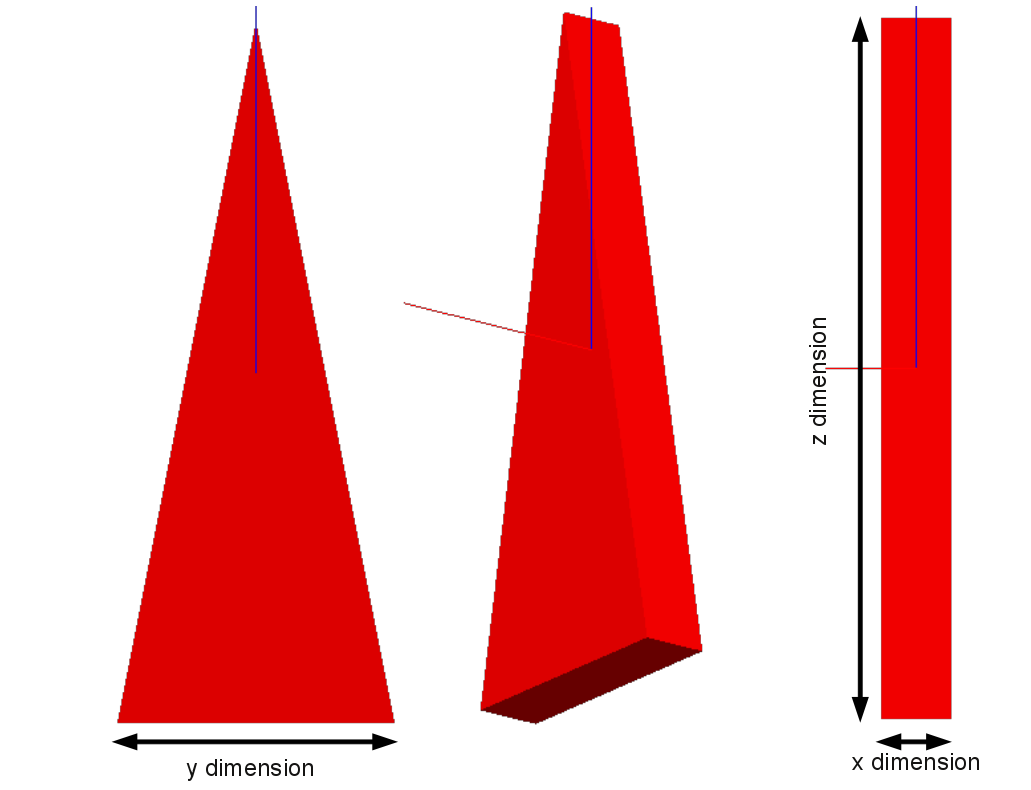
\includegraphics[width=13.968cm,height=8.394cm]{mice_modules/wedge_geometry.png}
\end{center}
\caption{Schematic of the geometry of a Wedge volume.}
\end{figure}
\begin{center}
\tablefirsthead{\hline
{\bfseries Property} &
{\bfseries Type} &
{\bfseries Description}\\}
\tablehead{\hline
{\bfseries Property} &
{\bfseries Type} &
{\bfseries Description}\\}
\tabletail{}
\tablelasttail{}
\begin{supertabular}{|m{3.665cm}|m{1.278cm}|m{12.052cm}|}
\hline
Dimensions &
Hep3

Vector &
\liststyleLxi
\begin{enumerate}
\item Width of the prism in x
\item Open end height of the prism in y
\item Length of the prism in z
\end{enumerate}
\\\hline
\end{supertabular}
\end{center}
\subsubsection{Volume Polycone}
A polycone is a volume of rotation, defined by a number of points in r and z. The volume is found by a linear
interpolation of the points.

\begin{center}
\tablefirsthead{\hline
{\bfseries Property} &
{\bfseries Type} &
{\bfseries Description}\\}
\tablehead{\hline
{\bfseries Property} &
{\bfseries Type} &
{\bfseries Description}\\}
\tabletail{}
\tablelasttail{}
\begin{supertabular}{|m{3.665cm}|m{1.278cm}|m{12.052cm}|}
\hline
PolyconeType &
string &
Set to Fill to define a solid volume of rotation. Set to Cone to define a shell volume of rotation with an inner and
outer surface.\\\hline
FieldMapMode &
string &
The name of the file that contains the polycone data.\\\hline
\end{supertabular}
\end{center}
\subsubsection{Volume Quadrupole}
Quadrupoles are defined by an empty cylinder with four further cylinders that are approximations to pole tips.

\begin{center}
\tablefirsthead{\hline
{\bfseries Property} &
{\bfseries Type} &
{\bfseries Description}\\}
\tablehead{\hline
{\bfseries Property} &
{\bfseries Type} &
{\bfseries Description}\\}
\tabletail{}
\tablelasttail{}
\begin{supertabular}{|m{3.665cm}|m{1.278cm}|m{12.052cm}|}
\hline
PhysicalLength &
double &
The length of the quadrupole container.\\\hline
QuadRadius &
double &
The distance from the quad centre to the outside of the quad.\\\hline
PoleTipRadius &
double &
The distance from the quad centre to the pole tip.\\\hline
CoilRadius &
double &
~
\\\hline
CoilHalfWidth &
double &
~
\\\hline
BeamlineMaterial &
string &
The material from which the beamline volume is made.\\\hline
QuadMaterial &
string &
The material from which the quadrupole volume is made.\\\hline
\end{supertabular}
\end{center}
\subsubsection{Volume Multipole}
Multipoles are defined by an empty box with an arbitrary number of cylinders that are approximations to pole tips. Poles
are placed around the centre of the box with n-fold symmetry. Multipoles can be curved, in which case poles cannot be
defined -- only a curved rectangular aperture will be present.

\begin{center}
\tablefirsthead{\hline
{\bfseries Property} &
{\bfseries Type} &
{\bfseries Description}\\}
\tablehead{\hline
{\bfseries Property} &
{\bfseries Type} &
{\bfseries Description}\\}
\tabletail{}
\tablelasttail{}
\begin{supertabular}{|m{3.892cm}|m{1.333cm}|m{11.77cm}|}
\hline
{\itshape ApertureCurvature} &
double &
Radius of curvature of the multipole aperture. For now curved apertures cannot have poles. Set to 0 for a straight
aperture.\\\hline
{\itshape ApertureLength} &
double &
Length of the multipole aperture.\\\hline
NumberOfPoles &
int &
Number of poles.\\\hline
PoleCentreRadius &
double &
The distance from the centre of the aperture to the centre of the cylindrical pole.\\\hline
PoleTipRadius &
double &
The distance from the centre of the aperture to the tip of the cylindrical pole.\\\hline
{\itshape ApertureInnerHeight} &
double &
The inner full height of the aperture.\\\hline
{\itshape ApertureInnerWidth} &
double &
The inner full width of the aperture.\\\hline
{\itshape AppertureOuterHeight} &
double &
The outer full height of the aperture.\\\hline
{\itshape ApertureOuterWidth} &
double &
The outer full width of the aperture.\\\hline
\end{supertabular}
\end{center}
\subsubsection{Volume Boolean}
Boolean volumes enable several volumes to be combined to make very sophisticated shapes from a number of elements.
Elements can be combined either by union, intersection or subtraction operations. A union creates a volume that is the
sum of two elements; an intersection creates a volume that covers the region where two volumes intersect each other;
and a subtraction creates a volume that contains all of one volume except the region that another volume sits in.

Boolean volumes combine volumes modelled by other MiceModules (submodules), controlled using the properties listed
below. Only the volume shape is used; position, rotation and field models etc are ignored. Materials, colours and other
relevant properties are all taken only from the Boolean Volume's properties.

Note that unlike in other parts of MAUS, submodules for use in Booleans (BaseModule, BooleanModule1, BooleanModule2
...) must be defined in a separate file, either defined in \$MICEFILES/Models/Modules or in the working directory.

Also note that visualisation of boolean volumes is rather unreliable. Unfortunately this is a feature of GEANT4. An
alternative technique is to use special virtual detectors to examine hits in boolean volumes.

\begin{center}
\tablefirsthead{\hline
{\bfseries Property} &
{\bfseries Type} &
{\bfseries Description}\\}
\tablehead{\hline
{\bfseries Property} &
{\bfseries Type} &
{\bfseries Description}\\}
\tabletail{}
\tablelasttail{}
\begin{supertabular}{|m{3.89cm}|m{1.333cm}|m{11.772cm}|}
\hline
{\itshape BaseModule} &
string &
Name of the physical volume that the BooleanVolume is based on. This volume will be placed at (0,0,0) with no rotation,
and all subsequent volumes will be added, subtracted or intersected with this one.\\\hline
{\itshape BooleanModule1} &
string &
The first module to add. MAUS will search for the MiceModule with path
\$MICEFILES/Models/Modules/{\textless}BooleanModule1{\textgreater}.\\\hline
{\itshape BooleanModule1Type} &
string &
The type of boolean operation to apply, either ``Union'', ``Intersection'' or ``Subtraction''.\\\hline
{\itshape BooleanModule1Pos} &
Hep3

Vector &
The position of the new volume with respect to the Base volume.\\\hline
{\itshape BooleanModule1Rot} &
Hep3

Vector &
The rotation of the new volume with respect to the Base volume.\\\hline
{\itshape BooleanModuleN} &
string &
Add extra modules as required. Replace ``N'' with the module number. N must be a continuous series incrementing by 1 for
each new module. Note that the order in which modules are added is important -- (A-B) \textsf{U }C is different to A-(B
\textsf{U }C).\\\hline
{\itshape BooleanModuleNType} &
\multicolumn{1}{m{1.333cm}}{string} &
\\\hhline{--~}
{\itshape BooleanModuleNPos} &
\multicolumn{1}{m{1.333cm}}{Hep3

Vector} &
\\\hhline{--~}
{\itshape BooleanModuleNRot} &
\multicolumn{1}{m{1.333cm}}{Hep3

Vector} &
\\\hhline{--~}
\end{supertabular}
\end{center}
\subsubsection{Volume Sphere}
A sphere is a spherical shell, with options for opening angles to make segments.

\begin{center}
\tablefirsthead{\hline
{\bfseries Property} &
{\bfseries Type} &
{\bfseries Description}\\}
\tablehead{\hline
{\bfseries Property} &
{\bfseries Type} &
{\bfseries Description}\\}
\tabletail{}
\tablelasttail{}
\begin{supertabular}{|m{3.89cm}|m{1.333cm}|m{11.772cm}|}
\hline
{\itshape Dimensions} &
Hep3

Vector &
The x value defines the inner radius. The y value defines the outer radius of the shell. The z value is not
used.\\\hline
Phi &
Hep3

Vector &
The x value defines the start opening angle in phi. The y value defines the end opening angle. The z value is not used.
Phi values must be in the range 0 to 360 degrees. If undefined, defaults to the range 0-360 degrees.\\\hline
Theta &
Hep3

Vector &
The x value defines the start opening angle in theta. The y value defines the end opening angle. The z value is not
used. Theta values must be in the range 0 to 180 degrees. If undefined, defaults to the range 0-360 degrees.\\\hline
\end{supertabular}
\end{center}

\subsection{Repeating Modules}
It is possible to set up a repeating structure for e.g. a repeating magnet lattice. The RepeatModule property enables
the user to specify that a particular module will be repeated a number of times, with all properties passed onto the
child module, but with a new position, orientation and scale factor. Each successive repetition will be given a
translation and a rotation relative to the coordinate system of the previous repetition, enabling the construction of
circular and straight accelerator lattices. Additionally, successive repetitions can have fields scaled relative to
previous repetitions, enabling for example alternating lattices.

\begin{center}
\tablefirsthead{\hline
{\bfseries Property} &
{\bfseries Type} &
{\bfseries Description}\\}
\tablehead{\hline
{\bfseries Property} &
{\bfseries Type} &
{\bfseries Description}\\}
\tabletail{}
\tablelasttail{}
\begin{supertabular}{|m{3.892cm}|m{1.333cm}|m{11.77cm}|}
\hline
{\itshape RepeatModule} &
bool &
Set to 1 to enable repeats in this module.\\\hline
{\itshape NumberOfRepeats} &
int &
Number of times the module will be repeated in addition to the initial placement.\\\hline
{\itshape RepeatTranslation} &
Hep3

Vector &
Translation applied to successive repeats, applied in the coordinate system of the previous repetition.\\\hline
{\itshape RepeatRotation} &
Hep3

Vector &
Rotation applied to successive repeats, applied in the coordinate system of the previous repetition.\\\hline
{\itshape RepeatScaleFactor} &
double &
ScaleFactor applied to successive repeats, applied relative to previous repetition's scale factor.\\\hline
\end{supertabular}
\end{center}
The RepeatModule2 property also enables the user to specify that a particular module will be repeated a number of times.
In this case, MAUS will set a substitution variable @RepeatNumber that holds an index between 0 and NumberOfRepeats.
This can be used in an expression in to provide a versatile interface between user and accelerator lattice.

\begin{center}
\tablefirsthead{\hline
{\bfseries Property} &
{\bfseries Type} &
{\bfseries Description}\\}
\tablehead{\hline
{\bfseries Property} &
{\bfseries Type} &
{\bfseries Description}\\}
\tabletail{}
\tablelasttail{}
\begin{supertabular}{|m{3.892cm}|m{1.333cm}|m{11.77cm}|}
\hline
{\itshape RepeatModule2} &
bool &
Set to 1 to enable repeats in this module.\\\hline
{\itshape NumberOfRepeats} &
int &
Number of times the module will be repeated in addition to the initial placement.\\\hline
\end{supertabular}
\end{center}

\subsection{Beam Definition and Beam Envelopes}
The Optics application can be used to track a trajectory and associated beam envelope through the accelerator structure.
Optics works by finding the Jacobian around some arbitrary trajectory using a numerical differentiation. This is used
to define a linear mapping about this trajectory, which can then be used to transport the beam envelope.

A beam envelope is defined by a reference trajectory and a beam ellipse. The reference trajectory takes its position and
direction from the position and rotation of the module. If no rotation is defined the reference trajectory is taken along
the z-axis. The magnitude of the momentum and the initial time of the reference trajectory is defined by properties. RF
cavities are phased using the reference trajectory defined here.

The beam ellipse is represented by a matrix, which can either be set using 

\begin{itemize}
\item Twiss-style parameters in $(x,px)$, $(y,py)$ and $(t,E)$ spaces.
\item Twiss-style parameters in $(t,E)$ space and Penn-style parameters in a cylindrically symmetric $(x,px,y,py)$ space.
\item A 6x6 beam ellipse matrix where the ellipse equation is given by $\mathbf{X}.\mathbf{T}() \mathbf{M} \mathbf{X} =
1$.
\end{itemize}
The Penn ellipse matrix is given by

\begin{equation*}
M=\left(\begin{matrix}\epsilon_Lmc\frac{\beta_L}{p}&-\epsilon_Lmc\alpha _L&0&0&0&0\\
       &\epsilon_Lmc\gamma_Lp&\frac{D_x}{E}V(E)&\frac{D_x'}{E}V(E)&\frac{D_y}{E}V(E)&\frac{D_y'}{E}V(E)\\
       &&\epsilon _Tmc\frac{\beta _T}{p}&-\epsilon_Tmc\alpha_T&0&-\epsilon _Tmc(\frac{q}{2}\beta _T\frac{B_z}{P}-L)\\
      &&&\epsilon _Tmc\gamma _Tp&\epsilon _Tmc(\frac{q}{
2}\beta _T\frac{B_z}{P}-L)&0\\&&&&\epsilon _Tmc\frac{\beta _T}{p}&-\epsilon _Tmc\alpha _T\\&&&&&\epsilon _Lmc\gamma
_Tp\end{matrix}\right)
\end{equation*}
Here $L$ is a normalised canonical angular momentum, $q$ is the reference particle charge,
$B_{z}$ is the nominal on-axis magnetic field, $p$ is the reference momentum,
$m$ is the reference mass, $\epsilon_T$ is the transverse emittance, $\beta_T$ and
$\alpha_{T}$ are the transverse Twiss-like functions, $\epsilon_{L}$ is the longitudinal emittance and
$\beta_{L}$ and $\alpha_{L}$ are the longitudinal Twiss-like functions. Additionally $D_{x}$,
$D_{y}$, $D'_{x}$ and $D'_{y}$ are the dispersions and their derivatives with respect to
$z$ and $V(E)$ is the variance of energy (given by the $(2,2)$ term in the matrix above).

The Twiss ellipse matrix is given by

\begin{equation*}
M=\left(\begin{matrix}\epsilon _Lmc\frac{\beta _L}{p}&-\epsilon _Lmc\alpha _L&0&0&0&0\\&\epsilon _Lmc\gamma
_Lp&\frac{D_x}{E}V(E)&\frac{D_x'}{E}V(E)&\frac{D_y}{E}V(E)&\frac{D_y'}{E}V(E)\\&&\epsilon _xmc\frac{\beta _x}{p}&-\epsilon
_xmc\alpha _x&0&0\\&&&\epsilon _xmc\gamma _xp&0&0\\&&&&\epsilon _ymc\frac{\beta _y}{p}&-\epsilon _ymc\alpha
_y\\&&&&&\epsilon _ymc\gamma _yp\end{matrix}\right)
\end{equation*}
Here \textit{p} is the reference momentum, \textit{m} is the reference mass, e\textsubscript{i}, b\textsubscript{i} and
a\textsubscript{i} are the emittances and Twiss functions in the (t,E), (x,p\textsubscript{x}) and
(y,p\textsubscript{y}) planes respectively, D\textsubscript{x}, D\textsubscript{y}, D'\textsubscript{x},
D'\textsubscript{y} are the dispersions and their derivatives with respect to z and V(E) is the variance of energy
(given by the (2,2) term in the matrix above).

\begin{center}
\tablefirsthead{\hline
{\bfseries Property} &
{\bfseries Type} &
{\bfseries Description}\\}
\tablehead{\hline
{\bfseries Property} &
{\bfseries Type} &
{\bfseries Description}\\}
\tabletail{}
\tablelasttail{}
\begin{supertabular}{|m{3.319cm}|m{1.2019999cm}|m{11.974cm}|}
\hline
{\itshape EnvelopeType} &
string &
Set to \textit{TrackingDerivative} to evolve a beam envelope in the Optics application.\\\hline
{\itshape BeamType} &
string &
Set to \textit{Random} to generate a beam using the parameters below for the Simulation application. Set to
\textit{Pencil }to generate a pencil beam (with no random distribution). Set to \textit{ICOOL}, \textit{Turtle,
MAUS\_PrimaryGenHit} or \textit{G4BeamLine} to use a beam file.\\\hline
{\itshape Pid} &
int &
The particle ID of particles in the envelope or beam.\\\hline
{\itshape Longitudinal}

{\itshape Variable} &
string &
Set the longitudinal variable used to define the reference trajectory momentum. Options are \textit{Energy},
\textit{KineticEnergy, Momentum} and\textit{ ZMomentum.}\\\hline
\multicolumn{1}{m{3.319cm}}{\hspace*{-\tabcolsep}\begin{tabular}{|m{3.319cm}}

Energy\\\hline
KineticEnergy\\\hline
Momentum\\\hline
ZMomentum\\\hline
\end{tabular}\hspace*{-\tabcolsep}
} &
\hspace*{-\tabcolsep}\begin{tabular}{|m{1.2019999cm}}

double\\\hline
double\\\hline
double\\\hline
double\\\hline
\end{tabular}\hspace*{-\tabcolsep}
 &
Define the value of the longitudinal variable used to calculate the mean momentum and energy. The usual relationship
E\textsuperscript{2}+p\textsuperscript{2}c\textsuperscript{2}=m\textsuperscript{2}c\textsuperscript{4} applies. Kinetic
energy E\textsubscript{k} is related to energy E by E\textsubscript{k}+m=E.\\\hhline{~~-}
{\itshape EllipseDefinition} &
string &
Define the beam ellipse that will be used in calculating the evolution of the Envelope, or used to generate a beam for
BeamType \textit{Random}. Options are \textit{Twiss, Penn} and\textit{ Matrix}.\\\hline
\multicolumn{3}{|m{16.894999cm}|}{{\itshape The following properties are only used if EllipseDefinition is set to
Twiss}}\\\hline
\multicolumn{2}{m{4.721cm}|}{\hspace*{-\tabcolsep}\begin{tabular}{|m{3.319cm}|m{1.2019999cm}}

{\itshape Emittance\_X} &
double\\\hline
{\itshape Emittance\_Y} &
double\\\hline
{\itshape Emittance\_L} &
double\\\hline
\end{tabular}\hspace*{-\tabcolsep}
} &
Emittance in each 2d subspace, (x,px), (y,py) and (t,E).\\\hhline{~~-}
\multicolumn{2}{m{4.721cm}|}{\hspace*{-\tabcolsep}\begin{tabular}{|m{3.319cm}|m{1.2019999cm}}

{\itshape Beta\_X} &
double\\\hline
{\itshape Beta\_Y} &
double\\\hline
{\itshape Beta\_L} &
double\\\hline
\end{tabular}\hspace*{-\tabcolsep}
} &
Twiss b function in each 2d subspace, (x,px), (y,py) and (t,E).\\\hhline{~~-}
\multicolumn{2}{m{4.721cm}|}{\hspace*{-\tabcolsep}\begin{tabular}{|m{3.319cm}|m{1.2019999cm}}

{\itshape Alpha\_X} &
double\\\hline
{\itshape Alpha\_Y} &
double\\\hline
{\itshape Alpha\_L} &
double\\\hline
\end{tabular}\hspace*{-\tabcolsep}
} &
Twiss a function in each 2d subspace, (x,px), (y,py) and (t,E).\\\hhline{~~-}
\multicolumn{3}{|m{16.894999cm}|}{{\itshape The following properties are only used if EllipseDefinition is set to
Matrix}}\\\hline
\multicolumn{2}{m{4.721cm}|}{\hspace*{-\tabcolsep}\begin{tabular}{|m{3.319cm}|m{1.2019999cm}}

{\itshape Covariance(t,t)} &
double\\\hline
{\itshape Covariance(t,E)} &
double\\\hline
{\itshape Covariance(t,x)} &
double\\\hline
{\itshape ...} &
double\\\hline
{\itshape Covariance(Py,Py)} &
double\\\hline
\end{tabular}\hspace*{-\tabcolsep}
} &
Set the 6x6 matrix that will be used in the to define the beam ellipse. Covariances should be covariances of elements of
the matrix (x,Px,y,Py,t,E).

\ This must be a positive definite matrix, i.e. determinant {\textgreater} 0. Note that this means that at least the 6
terms on the diagonal must be defined. Other terms default to 0.\\\hline
\multicolumn{3}{|m{16.894999cm}|}{{\itshape The following properties are only used if EllipseDefinition is set to
Penn}}\\\hline
{\itshape Emittance\_T} &
double &
Transverse emittance for the 4d (x,px,y,py) subspace.\\\hline
{\itshape Emittance\_L} &
double &
Longitudinal emittance for the 2d (t,E) subspace.\\\hline
{\itshape Beta\_T} &
double &
Transverse beta for the 4d (x,px,y,py) subspace.\\\hline
{\itshape Beta\_L} &
double &
Longitudinal beta for the 2d (t,E) subspace.\\\hline
{\itshape Alpha\_T} &
double &
Transverse alpha for the 4d (x,px,y,py) subspace.\\\hline
{\itshape Alpha\_L} &
double &
Longitudinal alpha for the 2d (t,E) subspace.\\\hline
{\itshape Normalised}

{\itshape AngularMomentu} &
double &
Normalised angular momentum for the transverse phase space.\\\hline
Bz &
double &
Nominal magnetic field on the reference particle.\\\hline
\multicolumn{3}{|m{16.894999cm}|}{{\itshape The following properties are used if EllipseDefinition is set to Penn or
Twiss}}\\\hline
Dispersion\_X &
double &
Dispersion in x (x-energy correlation).\\\hline
Dispersion\_Y &
double &
Dispersion in y (y-energy correlation).\\\hline
DispersionPrime\_X &
double &
D' in x (Px-energy correlation).\\\hline
DispersionPrime\_Y &
double &
D' in y (Py-energy correlation).\\\hline
\multicolumn{3}{|m{16.894999cm}|}{{\itshape The following properties are only relevant for generating a beam
envelope}}\\\hline
RootOutput &
string &
Output file name for writing output beam envelope in ROOT binary format.\\\hline
LongTextOutput &
string &
Output file name for writing output beam envelope in string format.\\\hline
ShortTextOutput &
string &
Output file name for writing output beam envelope in string format. This abbreviated output omits some of the fields
that are present in LongTextOutput files.\\\hline
BeamOutput &
string &
If a BeamType is defined, this property controls the file name to which beam data is written.\\\hline
Delta\_t &
double &
Offset in time used for calculating numerical derivatives. Default is 0.1 ns.\\\hline
Delta\_E &
double &
Offset in energy used for calculating numerical derivatives. Default is 1 MeV.\\\hline
Delta\_x &
double &
Offset in x position used for calculating numerical derivatives. Default is 1 mm.\\\hline
Delta\_Px &
double &
Offset in x momentum used for calculating numerical derivatives. Default is 1 MeV/c.\\\hline
Delta\_y &
double &
Offset in y position used for calculating numerical derivatives. Default is 1 mm.\\\hline
Delta\_Py &
double &
Offset in y momentum used for calculating numerical derivatives. Default is 1 MeV/c.\\\hline
\multicolumn{2}{m{4.721cm}|}{\hspace*{-\tabcolsep}\begin{tabular}{|m{3.319cm}|m{1.2019999cm}}

Max\_Delta\_t &
double\\\hline
Max\_Delta\_E &
double\\\hline
Max\_Delta\_x &
double\\\hline
Max\_Delta\_Px &
double\\\hline
Max\_Delta\_y &
double\\\hline
Max\_Delta\_Py &
double\\\hline
\end{tabular}\hspace*{-\tabcolsep}
} &
Maximum offsets when polyfit algorithm is used. In some cases the offset can keep increasing without limit unless these
maximum offsets are defined. Default is no limit.\\\hhline{~~-}
\multicolumn{3}{|m{16.894999cm}|}{{\itshape The following properties are only relevant for generating a particle
beam}}\\\hline
UseAsReference &
Bool &
If set to true and the datacard \textit{FirstParticleIsReference} is set to 0, the first event in the Module will be
used as the reference particle that sets cavity phases. This particle will then have the mean trajectory (i.e. no
gaussian distribution).\\\hline
{\itshape BeamFile} &
string &
If the BeamType is \textit{ICOOL}, \textit{Turtle, MAUS\_PrimaryGenHit} or \textit{G4BeamLine}, this property defines
the name of the file containing tracks for MAUS.\\\hline
NumberOfEvents &
int &
Set the maximum number of events to take from this module. If other modules are defined, MAUS will iterate over the
modules until it the datacard \textit{numEvts} is reached or all modules have been run to \textit{NumberOfEvents}.
Default is for MAUS to keep tracking from the first module it finds until \textit{numEvts} is reached.\\\hline
\end{supertabular}
\end{center}
\subsection{Optimiser}
It is possible to define an optimiser for use in the Optics application. The optimiser enables the user to vary
parameters in the MiceModule file and try to find some optimum setting. For each value of the parameters, MAUS Optics
will calculate a score; the optimiser attempts to find a minimum value for this score.

\begin{center}
\tablefirsthead{\hline
{\bfseries Property} &
{\bfseries Type} &
{\bfseries Description}\\}
\tablehead{\hline
{\bfseries Property} &
{\bfseries Type} &
{\bfseries Description}\\}
\tabletail{}
\tablelasttail{}
\begin{supertabular}{|m{3.319cm}|m{1.2019999cm}|m{11.974cm}|}
\hline
{\itshape Optimiser} &
string &
Controls the function used for optimising. For now Minuit is the only available option.\\\hline
{\itshape Algorithm} &
string &
For \textit{Minuit} optimiser, controls the \textit{Minuit} algorithm used. In general Simplex is a good option to use
here. An alternative is Migrad. See Minuit documentation (for example at http://root.cern.ch/root/html/TMinuit.html)
for further information. Minuit attempts to minimise the score function defined by the Score properties.\\\hline
{\itshape NumberOfTries} &
int &
Maximum number of iterations MAUS will make in order to find the optimum value.\\\hline
{\itshape StartError} &
double &
Guess at the initial error in the score.\\\hline
{\itshape EndError} &
double &
Required final error in the score for the optimisation to converge successfully.\\\hline
RebuildSimulation &
bool &
Set to False to tell MAUS not to rebuild the simulation on each iteration. This should be used to speed up the
optimiser when a parameter is used that does not change the field maps. Default is true.\\\hline
{\itshape Parameter1\_Start} &
double &
Seed value for the parameter, that is used in the first iteration.\\\hline
{\itshape Parameter1\_Name} &
string &
Name of the parameter. This name is used as an expression substitution variable elsewhere in the code and should start
with @. See Expression Substitutions above for details on usage of expression substitutions.\\\hline
Parameter1\_Delta &
double &
Estimated initial error on the parameter. Default is 1.\\\hline
Parameter1\_Fixed &
bool &
Set to true to fix the parameter (so that it is excluded from the optimisation). Default is false.\\\hline
Parameter1\_Min &
double &
If required, set to the minimum value that the parameter can hold.\\\hline
Parameter1\_Max &
double &
If required, set to the maximum value that the parameter can hold.\\\hline

\multicolumn{2}{m{4.721cm}}{\hspace*{-\tabcolsep}\begin{tabular}{|m{3.319cm}|m{1.2019999cm}|}

Parameter2\_Start &
...\\\hline
... &
...\\\hline
Parameter2\_Max &
...\\\hline
{\itshape Score1} &
double\\\hline
Score2 &
...\\\hline
... &
...\\\hline
\end{tabular}\hspace*{-\tabcolsep}
} &
Define an arbitrary number of parameters. Parameters must be numbered consecutively, and each parameter must have at
least the start value and name defined. The optimiser will attempt to optimise against a score that is calculated by summing the Score1, Score2,... parameters
on each iteration.\\\hline
\end{supertabular}
\end{center}
 % how to set up a geometry
\chapter{Field Properties}
Invoke a field using PropertyString FieldType {\textless}fieldtype{\textgreater}. The field will be placed, normally
centred on the MiceModule Position and with the appropriate Rotation. Further options for each field type are specified
below, and relevant datacards are also given. If a fieldtype is specified some other properties must also be specified,
while others may be optional, usually taking their value from defaults specified in the datacards. Only one fieldtype
can be specified per module. However, fields from multiple modules are superimposed, each transformed according to the
MiceModule specification. This enables many different field configurations to be simulated using MAUS.

To use BeamTools fields, datacard FieldMode Full must be set. This is the default.

\begin{center}
\tablefirsthead{\hline
{\bfseries Property} &
{\bfseries Type} &
{\bfseries Description}\\}
\tablehead{\hline
{\bfseries Property} &
{\bfseries Type} &
{\bfseries Description}\\}
\tabletail{}
\tablelasttail{}
\begin{supertabular}{|m{3.665cm}|m{1.278cm}|m{12.052cm}|}
\hline
{\itshape FieldType} &
string &
Set the field type of the MiceModule.\\\hline
\end{supertabular}
\end{center}
\subsection{FieldType CylindricalField}
Sets a constant magnetic field in a cylindrical region symmetric about the z-axis of the module.

\begin{center}
\tablefirsthead{\hline
{\bfseries Property} &
{\bfseries Type} &
{\bfseries Description}\\}
\tablehead{\hline
{\bfseries Property} &
{\bfseries Type} &
{\bfseries Description}\\}
\tabletail{}
\tablelasttail{}
\begin{supertabular}{|m{3.665cm}|m{1.278cm}|m{12.052cm}|}
\hline
{\itshape ConstantField} &
Hep3

Vector &
The magnetic field that will be placed in the region.\\\hline
\multicolumn{2}{m{5.143cm}|}{\hspace*{-\tabcolsep}\begin{tabular}{|m{3.665cm}|m{1.278cm}}

{\itshape Length} &
double\\\hline
{\itshape Radius} &
double\\\hline
\end{tabular}\hspace*{-\tabcolsep}
} &
The physical extent of the region.\\\hhline{~~-}
\end{supertabular}
\end{center}
\subsection{FieldType RectangularField}
Sets a constant magnetic field in a rectangular region.

\begin{center}
\tablefirsthead{\hline
{\bfseries Property} &
{\bfseries Type} &
{\bfseries Description}\\}
\tablehead{\hline
{\bfseries Property} &
{\bfseries Type} &
{\bfseries Description}\\}
\tabletail{}
\tablelasttail{}
\begin{supertabular}{|m{3.665cm}|m{1.278cm}|m{12.052cm}|}
\hline
{\itshape ConstantField} &
Hep3

Vector &
The magnetic field that will be placed in the region.\\\hline
\multicolumn{2}{m{5.143cm}|}{\hspace*{-\tabcolsep}\begin{tabular}{|m{3.665cm}|m{1.278cm}}

{\itshape Length} &
double\\\hline
{\itshape Width} &
double\\\hline
{\itshape Height} &
double\\\hline
\end{tabular}\hspace*{-\tabcolsep}
} &
The physical extent of the region.\\\hhline{~~-}
\end{supertabular}
\end{center}
\subsection{FieldType Solenoid}
MAUS simulates solenoids using a series of current sheets. The field for each solenoid is written to a field map on a
rectangular grid and can then be reused. The field from each current sheet is calculated using the formula for current
sheets detailed in MUCOOL Note 281, \textit{Modeling solenoids using coil, sheet and block conductors}.

\begin{center}
\tablefirsthead{\hline
{\bfseries Property} &
{\bfseries Type} &
{\bfseries Description}\\}
\tablehead{\hline
{\bfseries Property} &
{\bfseries Type} &
{\bfseries Description}\\}
\tabletail{}
\tablelasttail{}
\begin{supertabular}{|m{3.665cm}|m{1.278cm}|m{12.052cm}|}
\hline
{\itshape FileName} &
string &
Read or write solenoid data to the filename. If different modules have the same filename, MAUS assumes they are the
same.\\\hline
FieldMapMode &
string &
If set to Read, MAUS will attempt to read existing data from the FileName. If set to Write, MAUS will generate new
data and write it to the FileName. If set to Analytic, MAUS will calculate fields directly without interpolating. If
set to WriteDynamic acts as in Write except the grid extent and grid spacing at each point is chosen dynamically to
some tolerance defined in the FieldTolerance property. Takes default from datacard SolDataFiles (Write).\\\hline
\multicolumn{2}{m{5.143cm}|}{\hspace*{-\tabcolsep}\begin{tabular}{|m{3.665cm}|m{1.278cm}}

{\itshape Length} &
double\\\hline
{\itshape Thickness} &
double\\\hline
{\itshape InnerRadius} &
double\\\hline
{\itshape CurrentDensity} &
double\\\hline
\end{tabular}\hspace*{-\tabcolsep}
} &
Coil physical parameters. Only used in Write/Analytic mode where they are mandatory.\\\hhline{~~-}
ZExtentFactor &
double &
Field map extends to length + ZExtentFactor*innerRadius in Write mode. Takes default from datacard SolzMapExtendFactor
(10.). Map size is chosen dynamically in WriteDynamic mode.\\\hline
RExtentFactor &
double &
Field map extends to radius RExtentFactor*innerRadius in Write mode. Takes default from datacard SolrMapExtendFactor
(2.018...). Avoid allowing grid nodes to fall on sheets.\\\hline
NumberOfZCoords &
int &
Number of coordinates in \textit{z} in field map grid in Write mode. Takes default from datacard NumberNodesZGrid
(500).\\\hline
NumberOfRCoords &
int &
Number of coordintes in \textit{r} in field map grid in Write mode. Takes default from datacard NumberNodesRGrid
(100).\\\hline
NumberOfSheets &
int &
Number of sheets used to calculate the field. Takes default from datacard DefaultNumberOfSheets (10).\\\hline
{\itshape FieldTolerance } &
double &
Mandatory when FieldMapMode is WriteDynamic. If field map mode is write dynamic, this datacard controls the tolerance on
errors in the field with which the field grid and the grid extent will be chosen. \\\hline
Interpolation

Algorithm &
string &
Choose the interpolation algorithm. Options are BiLinear for a linear interpolation in \textit{r} and \textit{z}, or
LinearCubic \ for a linear interpolation in \textit{r} and a cubic spline in \textit{z}. Default is
LinearCubic.\\\hline
IsAmalgamated &
bool &
Set to 1 to add the coil to CoilAmalgamtion parent field (see below).\\\hline
\end{supertabular}
\end{center}

\subsection{FieldType FieldAmalgamation}
During tracking, MAUS stores a list of fields and for each one MAUS checks to see if tracking is performed through a
particular field map's bounding box. This can be slow if a large number of fields are present. One way to speed this up
is to store contributions from many coils in a single CoilAmalgamation. A CoilAmalgamation searches through child
modules for solenoids with PropertyBool IsAmalgamated set to true. If it finds such a coil, it will add the field
generated by the solenoid to its own field map and disable the coil.

\begin{center}
\tablefirsthead{\hline
{\bfseries Property} &
{\bfseries Type} &
{\bfseries Description}\\}
\tablehead{\hline
{\bfseries Property} &
{\bfseries Type} &
{\bfseries Description}\\}
\tabletail{}
\tablelasttail{}
\begin{supertabular}{|m{3.665cm}|m{1.278cm}|m{12.052cm}|}
\hline
{\itshape Length} &
double &
The Length of the field map generated by the CoilAmalgamation.\\\hline
{\itshape RMax} &
double &
The maximum radius of the field map generated by the CoilAmalgamation.\\\hline
Interpolation

Algorithm &
string &
Choose the interpolation algorithm. Options are BiLinear for a linear interpolation in \textit{r} and \textit{z}, or
LinearCubic \ for a linear interpolation in \textit{r} and a cubic spline in \textit{z}. Default is
LinearCubic.\\\hline
\multicolumn{2}{m{5.143cm}|}{\hspace*{-\tabcolsep}\begin{tabular}{|m{3.665cm}|m{1.278cm}}

{\itshape ZStep} &
double\\\hline
{\itshape RStep} &
double\\\hline
\end{tabular}\hspace*{-\tabcolsep}
} &
Step size of the field map generated by the CoilAmalgamation.\\\hhline{~~-}
\end{supertabular}
\end{center}

\subsection{FieldType DerivativesSolenoid}
This is an alternative field model for solenoids that uses a power law expansion of the on-axis magnetic field and its
derivatives, and an exponential fall-off for the fringe field. The fringe field is defined in the same way as other end
fields, but note that HardEdged end field type is not available for solenoids and will result in an error.

\begin{center}
\tablefirsthead{\hline
{\bfseries Property} &
{\bfseries Type} &
{\bfseries Description}\\}
\tablehead{\hline
{\bfseries Property} &
{\bfseries Type} &
{\bfseries Description}\\}
\tabletail{}
\tablelasttail{}
\begin{supertabular}{|m{3.665cm}|m{1.278cm}|m{12.052cm}|}
\hline
{\itshape PeakField} &
double &
Nominal peak field of the solenoid.\\\hline
{\itshape ZMax} &
double &
Maximum z-half length of the solenoid bounding box in the local coordinate system of the magnet.\\\hline
{\itshape RMax} &
double &
Maximum radius of the solenoid bounding box in the local coordinate system of the magnet.\\\hline
{\itshape MaxEndPole} &
int &
Maximum derivative used in calculating the end field of the solenoid.\\\hline
\end{supertabular}
\end{center}
\subsection{Phasing Models}
MAUS has a number of sophisticated models for phasing RF cavities. These powerful models can make setting up RF
cavities with realistic fields both quick and easy.

When CavityMode is Unphased, MAUS attempts to phase the cavity itself. When using CavityMode Unphased MAUS needs to
know when particles enter, cross the middle, and leave cavities. This means that:

\liststyleLxiii
\begin{itemize}
\item The cavity must sit in a rectangular or cylindrical physical volume.
\item No other physical volumes may overlap or sit within the physical volume of the cavity.
\end{itemize}
If these conditions are not met the phasing algorithm is likely to fail.

To phase a cavity, MAUS builds a volume in the centre of the cavity that is used for phasing and then fires a
reference particle through the system. Stochastic processes are always disabled during this process, while mean energy
loss can be disabled using the datacard ReferenceEnergyLossModel. If a reference particle crosses a plane through the
centre of a cavity, it sets the phase of the cavity to the time at which the particle crosses. 

The field of the cavity during phasing is controlled by the property FieldDuringPhasing. There are four modes:

\liststyleLxiv
\begin{itemize}
\item \textit{None}: Cavity fields are disabled during phasing
\item \textit{Electrostatic}: An electrostatic field with no positional dependence given by
PeakEField*sin(ReferenceParticlePhase) is enabled during phasing.
\item \textit{TimeVarying}: A standard time varying field is applied during phasing, initially with arbitrary phase
relative to the reference particle. MAUS uses a Newton-Raphson method to find the appropriate reference phase
iteratively, with tolerance set by the datacard PhaseTolerance.
\item \textit{EnergyGainOptimised}: A standard time varying field is applied during phasing, initially with arbitrary
phase and peak field relative to the reference particle. MAUS uses a 2D Newton-Raphson method to find the appropriate
reference phase and peak field iteratively, so that the reference particle crosses the cavity centre with phase given
by property ReferenceParticlePhase and gains energy over the whole cavity given by property EnergyGain with tolerances
set by the datacards PhaseTolerance and RFDeltaEnergyTolerance.
\end{itemize}
\subsection{Tracking Stability Around RF Cavities}
Usually RF cavities have little or no fringe field, and this can lead to some instability in the tracking algorithms.
When MAUS makes a step into an RF cavity volume, the tracking algorithms tend to smooth out a field in a non-physical
way. This can be prevented by either (i) making the step size rather small in the RF cavity or (ii) forcing MAUS to
stop tracking by adding a physical volume at the entrance of the RF cavity (a window, typically made of vacuum). Doing
this should improve stability of tracking.

\subsection{FieldType PillBox}
Sets a PillBox field in a particular region. MAUS represents pillboxes using a sinusoidally varying TM010 pill box
field, with non-zero field vector elements given by

\begin{equation*}
\begin{gathered}B_{\phi }=J_1(k_rr)\cos (\omega t)\\E_z=J_0(k_rr)\cos (\omega t)\end{gathered}
\end{equation*}
Here J\textsubscript{n} are Bessel functions and k\textsubscript{r} is a constant. See, for example, SY Lee VI.1. All
other fields are 0.

\begin{center}
\tablefirsthead{\hline
{\bfseries Property} &
{\bfseries Type} &
{\bfseries Description}\\}
\tablehead{\hline
{\bfseries Property} &
{\bfseries Type} &
{\bfseries Description}\\}
\tabletail{}
\tablelasttail{}
\begin{supertabular}{|m{3.665cm}|m{1.278cm}|m{12.052cm}|}
\hline
{\itshape Length} &
double &
Length of the region in which the field is present.\\\hline
{\itshape CavityMode} &
string &
Phasing mode of the cavity - options are Phased, Unphased and Electrostatic.\\\hline
{\itshape FieldDuringPhasing} &
string &
Controls the field during cavity phasing -- options are None, Electrostatic, TimeVarying and
EnergyGainOptimised.\\\hline
{\itshape EnergyGain} &
double &
WhenFieldDuringPhasing is set to EnergyGainOptimised, controls the peak electric field.\\\hline
{\itshape Frequency} &
double &
The cavity frequency.\\\hline
{\itshape PeakEField} &
double &
The peak field of the cavity. Not used when the FieldDuringPhasing is EnergyGainOptimised.\\\hline
{\itshape TimeDelay} &
double &
In Phased mode the time delay (absolute time) of the cavity.\\\hline
PhasingVolume &
string &
Set to SpecialVirtual to make the central volume a special virtual.\\\hline
\multicolumn{2}{m{5.143cm}|}{\hspace*{-\tabcolsep}\begin{tabular}{|m{3.665cm}|m{1.278cm}}

ReferenceParticle

Energy &
double\\\hline
ReferenceParticle

Charge &
double\\\hline
\end{tabular}\hspace*{-\tabcolsep}
} &
In Electrostatic mode, MAUS calculates the peak field and the field the reference particle sees using a combination of
the reference particle energy, charge and phase. Take defaults from datacards NominalKineticEnergy and MuonCharge
\\\hhline{~~-}
ReferenceParticle

Phase &
double &
MAUS tries to phase the field so that the reference particle crosses the cavity at ReferenceParticlePhase (units are
angular). 0\textsuperscript{o} corresponds to no energy gain, 90\textsuperscript{o} corresponds to operation on-crest.
Default from datacard rfAcclerationPhase.\\\hline
\end{supertabular}
\end{center}
\subsection{FieldType RFFieldMap}
Sets a cavity with an RF field map in a particular region. RFFieldMap uses the same phasing algorithm as described
above.

\begin{center}
\tablefirsthead{\hline
{\bfseries Property} &
{\bfseries Type} &
{\bfseries Description}\\}
\tablehead{\hline
{\bfseries Property} &
{\bfseries Type} &
{\bfseries Description}\\}
\tabletail{}
\tablelasttail{}
\begin{supertabular}{|m{3.665cm}|m{1.278cm}|m{12.052cm}|}
\hline
{\itshape Length} &
double &
Length of the region in which the field is present.\\\hline
{\itshape CavityMode} &
string &
Phasing mode of the cavity - options are Phased and Unphased. RFFieldMaps cannot operated in Electrostatic mode.\\\hline
{\itshape FieldDuringPhasing} &
string &
Controls the field during cavity phasing -- options are None, Electrostatic, TimeVarying and
EnergyGainOptimised.\\\hline
{\itshape EnergyGain} &
double &
WhenFieldDuringPhasing is set to EnergyGainOptimised, controls the peak electric field.\\\hline
{\itshape Frequency} &
double &
The cavity frequency.\\\hline
{\itshape PeakEField} &
double &
The peak field of the cavity. Not used when the FieldDuringPhasing is EnergyGainOptimised.\\\hline
{\itshape TimeDelay} &
double &
In Phased mode the time delay (absolute time) of the cavity.\\\hline
PhasingVolume &
string &
Set to SpecialVirtual to make the central volume a special virtual.\\\hline
\multicolumn{2}{m{5.143cm}|}{\hspace*{-\tabcolsep}\begin{tabular}{|m{3.665cm}|m{1.278cm}}

ReferenceParticle

Energy &
double\\\hline
ReferenceParticle

Charge &
double\\\hline
\end{tabular}\hspace*{-\tabcolsep}
} &
In Electrostatic mode, MAUS calculates the peak. field and the field the reference particle sees using a combination
of the reference particle energy, charge and phase. Take defaults from datacards NominalKineticEnergy and MuonCharge
\\\hhline{~~-}
ReferenceParticle

Phase &
double &
MAUS tries to phase the field so that the reference particle crosses the cavity at ReferenceParticlePhase (units are
angular). 0\textsuperscript{o} corresponds to no energy gain, 90\textsuperscript{o} corresponds to operation on-crest.
Default from datacard rfAcclerationPhase.\\\hline
{\itshape FileName} &
string &
The file name of the field map file.\\\hline
{\itshape FileType} &
string &
The file type of the field map. Only supported option is SuperFishSF7.\\\hline
\end{supertabular}
\end{center}

\subsection{FieldType Multipole}
Creates a multipole of arbitrary order. Fields are generated using either a hard edged model, with no fringe fields at
all; or an Enge model similar to ZGoubi and COSY. In the former case fields are calculated using a simple polynomial
expansion. In the latter case fields are calculated using the polynomial expansion with an additional exponential drop
off. Fields can be superimposed onto a bent coordinate system to generate a sector multipole with arbitrary fixed
radius of curvature.

Unlike most other field models in MAUS, the zero position corresponds to the center of the entrance of the multipole;
and the multipole extends in the +z direction.

The method to define end fields is described in the section EndFieldTypes below

\begin{center}
\tablefirsthead{\hline
{\bfseries Property} &
{\bfseries Type} &
{\bfseries Description}\\}
\tablehead{\hline
{\bfseries Property} &
{\bfseries Type} &
{\bfseries Description}\\}
\tabletail{}
\tablelasttail{}
\begin{supertabular}{|m{3.691cm}|m{1.252cm}|m{12.052cm}|}
\hline
{\itshape Pole} &
int &
The reference pole of the magnet. 1=dipole, 2=quadrupole, 3=sextupole etc.\\\hline
{\itshape FieldStrength} &
double &
Scale the field strength in the good field region. For dipoles, this sets the dipole field; for quadrupoles this sets
the field gradient. Note that for some end field settings there can be no good field region (e.g. if the end length is
{\textgreater}\~{} centre length).\\\hline
{\itshape Height} &
double &
Height of the field region.\\\hline
{\itshape Width} &
double &
Width or delta radius of the field region.\\\hline
{\itshape Length} &
double &
Length of the field along the bent trajectory.\\\hline
EndFieldType &
string &
Set to HardEdged to disable fringe fields. Set to Enge or Tanh to use those models, as described elsewhere. Default is
HardEdged.\\\hline
CurvatureModel &
string &
Choose the model for curvature. Straight forces no curvature. Constant gives a constant radius of curvature;
StraightEnds gives a constant radius of curvature along the length of the multipole with straight end fields beyond
this length. MomentumBased gives radius of curvature determined by a momentum and a total bending angle.\\\hline
ReferenceCurvature &
double &
Radius of curvature of the magnet in Constant or StraightEnds mode. Set to 0 for a straight magnet. Default is
0.\\\hline
ReferenceMomentum &
double &
Reference momentum used to calculate the radius of curvature of a dipole in MomentumBased mode. Default is 0.\\\hline
{\itshape BendingAngle} &
double &
The angle used to calculate the radius of curvature of a dipole in MomentumBased mode. Note that this is mandatory in
MomentumBased mode.\\\hline
\end{supertabular}
\end{center}

\subsection{FieldType CombinedFunction}
This creates superimposed dipole, quadrupole and sextupole fields with a common radius of curvature. The field is
intended to mimic the first few terms in a multipole expansion of a field like

\begin{equation*}
B(y=0)=B_0\left(\frac r{r_0}\right)^k
\end{equation*}
The field index is a user defined parameter, while the dipole field and radius of curvature can either be defined
directly by the user or defined in terms of a reference momentum and total bending angle. Fields are calculated as in
the multipole field type defined above.

\begin{center}
\tablefirsthead{\hline
{\bfseries Property} &
{\bfseries Type} &
{\bfseries Description}\\}
\tablehead{\hline
{\bfseries Property} &
{\bfseries Type} &
{\bfseries Description}\\}
\tabletail{}
\tablelasttail{}
\begin{supertabular}{|m{3.689cm}|m{1.252cm}|m{12.054cm}|}
\hline
{\itshape Pole} &
int &
The reference pole of the magnet. 1=dipole, 2=quadrupole, 3=sextupole etc.\\\hline
{\itshape BendingField} &
double &
The nominal dipole field \textit{B}\textit{\textsubscript{0}}. Note that this is mandatory in all cases except where
CurvatureModel is MomentumBased, when the BendingAngle and ReferenceMomentum is used to calculate the \ dipole field
instead.\\\hline
{\itshape FieldIndex} &
double &
The field index \textit{k}.\\\hline
{\itshape Height} &
double &
Height of the field region.\\\hline
{\itshape Width} &
double &
Width or delta radius of the field region.\\\hline
{\itshape Length} &
double &
Length of the field along the bent trajectory.\\\hline
EndFieldType &
string &
Set to HardEdged to disable fringe fields. Set to Enge or Tanh to use those models, as described elsewhere. Default is
HardEdged.\\\hline
CurvatureModel &
string &
Choose the model for curvature. Straight forces no curvature. Constant gives a constant radius of curvature;
StraightEnds gives a constant radius of curvature along the length of the multipole with straight end fields beyond
this length. MomentumBased gives radius of curvature determined by a momentum and a total bending angle.\\\hline
ReferenceCurvature &
double &
Radius of curvature of the magnet in Constant or StraightEnds mode. Set to 0 for a straight magnet. Default is
0.\\\hline
ReferenceMomentum &
double &
Reference momentum used to calculate the radius of curvature of a dipole in MomentumBased mode. Default is 0.\\\hline
{\itshape BendingAngle} &
double &
The angle used to calculate the radius of curvature of a dipole in MomentumBased mode. Note that this is mandatory in
MomentumBased mode.\\\hline
\end{supertabular}
\end{center}

\subsection{EndFieldTypes}
In the absence of current sources, the magnetic field can be calculated from a scalar potential using the standard
relation

\begin{equation*}
\vec B=\nabla V_n
\end{equation*}
The scalar magnetic potential of the n\textsuperscript{th}{}-order multipole field is given by

\begin{equation*}
V_n=\sum _{q=0}^{q_m}\sum _{m=0}^nn!^2\frac{G^{(2q)}(s)(r^2+y^2)^q\sin (\frac{m\pi } 2)r^{n-m}y^m}{4^qq!(n+q)!m!(n-m)!}
\end{equation*}
where \textit{G(s)} is either the double Enge function,

\begin{equation*}
G(s)=E[(x-x_0)/\lambda ]+E[(-x-x_0)/\lambda ]-1
\end{equation*}
\begin{equation*}
E(s)=\frac{B_0}{R_0^n}\frac 1{1+\exp (C_1+C_2s+C_3s^2+...)}
\end{equation*}
or G(s) is the double tanh function,

\begin{equation*}
G(s)=\tanh [(x+x_0)/\lambda ]/2+\tanh [(x-x_0)/\lambda ]/2
\end{equation*}
and \textit{(r, y, s)} is the position vector in the rotating coordinate system. Note that here s is the distance from
the nominal end of the field map.

\begin{center}
\tablefirsthead{\hline
{\bfseries Property} &
{\bfseries Type} &
{\bfseries Description}\\}
\tablehead{\hline
{\bfseries Property} &
{\bfseries Type} &
{\bfseries Description}\\}
\tabletail{}
\tablelasttail{}
\begin{supertabular}{|m{3.689cm}|m{1.252cm}|m{12.054cm}|}
\hline
EndFieldType &
string &
Set to HardEdged to disable fringe fields. Set to Enge or Tanh to use those models, as described elsewhere. Default is
HardEdged.\\\hline
\multicolumn{3}{|m{17.394999cm}|}{{\itshape The following properties are used for EndFieldType Tanh}}\\\hline
EndLength &
double &
Set the l parameter that defines the rapidity of the field fall off.\\\hline
CentreLength &
double &
Set the \textit{x}\textit{\textsubscript{0}} parameter that defines the length of the flat field region.\\\hline
MaxEndPole &
int &
Set the maximum pole that will be calculated -- should be larger than the multipole pole.\\\hline
\multicolumn{3}{|m{17.394999cm}|}{{\itshape The following properties are used for EndFieldType Enge}}\\\hline
EndLength &
double &
Set the l parameter that defines the rapidity of the field fall off.\\\hline
CentreLength &
double &
Set the \textit{x}\textit{\textsubscript{0}} parameter that defines the length of the flat field region.\\\hline
MaxEndPole &
int &
Set the maximum pole that will be calculated -- should be larger than the multipole pole.\\\hline
\multicolumn{2}{m{5.1410003cm}|}{\hspace*{-\tabcolsep}\begin{tabular}{|m{3.689cm}|m{1.252cm}}

Enge1 &
double\\\hline
Enge2 &
double\\\hline
... &
double\\\hline
EngeN &
double\\\hline
\end{tabular}\hspace*{-\tabcolsep}
} &
Set the parameters C\textsubscript{i} as defined in the Enge function above.\\\hhline{~~-}
\end{supertabular}
\end{center}
\subsection{FieldType MagneticFieldMap}
Reads or writes a magnetic field map in a particular region. Two sorts of field maps are supported; either a 2d field
map, in which cylindrical symmetry is assumed, or a 3d field map. 

For 2d field maps, MAUS reads or writes a file that contains information about the radial and longitudinal field
components. This is intended for solenoidal field maps where only radial and longitudinal field components are present.
Note that in write mode, MAUS assumes cylindrical symmetry of the fields. In this case, MAUS writes the \textit{x}
and \textit{z} components of the magnetic field at points on a grid in \textit{x} and \textit{z}. Fields with an
electric component are excluded from this summation.

For 3d field maps, MAUS reads a file that contains the position and field in cartesian coordinates and performs a
linear interpolation. This requires quite large field map files; the file size can be slightly reduced by using certain
symmetries, as described below. It is currently not possible to write 3d field maps.

\begin{center}
\tablefirsthead{\hline
{\bfseries Property} &
{\bfseries Type} &
{\bfseries Description}\\}
\tablehead{\hline
{\bfseries Property} &
{\bfseries Type} &
{\bfseries Description}\\}
\tabletail{}
\tablelasttail{}
\begin{supertabular}{|m{3.665cm}|m{1.278cm}|m{12.052cm}|}
\hline
{\itshape FieldMapMode} &
string &
Set to Read to read a field map; and Write to write a field map.\\\hline
{\itshape FileName} &
string &
The file name that is used for reading or writing.\\\hline
FileType &
string &
The file format. Supported options in Read mode are MAUStext, MAUSbinary, g4beamline, icool, g4bl3dGrid. Only
MAUStext is supported in Write mode. Default is MAUStext.\\\hline
Symmetry &
string &
Symmetry option for g4bl3dGrid file type. Options are None, Dipole or Quadrupole. None uses the field map as is, while
Dipole and Quadrupole reflect the octant between the positive \textit{x}, \textit{y} and \textit{z} axes to give an
appropriate field for a dipole or quadrupole.\\\hline
\multicolumn{2}{m{5.143cm}|}{\hspace*{-\tabcolsep}\begin{tabular}{|m{3.665cm}|m{1.278cm}}

{\itshape ZStep} &
double\\\hline
{\itshape RStep} &
double\\\hline
\end{tabular}\hspace*{-\tabcolsep}
} &
Step size in \textit{z} and \textit{r}. Mandatory in Write mode but not used in Read mode (where step size comes from
the map file).\\\hhline{~~-}
\multicolumn{2}{m{5.143cm}|}{\hspace*{-\tabcolsep}\begin{tabular}{|m{3.665cm}|m{1.278cm}}

{\itshape ZMin} &
double\\\hline
{\itshape ZMax} &
double\\\hline
{\itshape RMin} &
double\\\hline
{\itshape RMax} &
double\\\hline
\end{tabular}\hspace*{-\tabcolsep}
} &
Upper and lower bounds in \textit{z} and \textit{r}. Mandatory in Write mode but not used in Read mode (where boundaries
come from the map file).\\\hhline{~~-}
\end{supertabular}
\end{center}
Some file formats are described below. I am working towards making the file format more generic and hence possibly
easier to use, but backwards compatibility will hopefully be maintained. 

\subsubsection{MAUStext Field Map Format}
The native field map format used by MAUS in text mode is described below.

{\ttfamily
\# GridType = Uniform N = \textbf{number\_rows}}

{\ttfamily
\# Z1 = \textbf{z\_start} Z2 = \textbf{z\_end} dZ = \textbf{z\_step}}

{\ttfamily
\# R1 = \textbf{r\_start} R2 = \textbf{r\_end} dR = \textbf{r\_step}}

{\ttfamily\bfseries
Bz\_Values\ \ Br\_Values}

{\ttfamily\bfseries
...\ \ \ \ ...}

{\ttfamily\bfseries
{\textless}Repeat as necessary{\textgreater}}

In this mode, field maps are represented by field values on a regular 2d grid that is assumed to have solenoidal
symmetry, i.e. cylindrical symmetry with no tangential component.

\begin{center}
\tablefirsthead{\hline
{\bfseries Name} &
{\bfseries Type} &
{\bfseries Description}\\}
\tablehead{\hline
{\bfseries Name} &
{\bfseries Type} &
{\bfseries Description}\\}
\tabletail{}
\tablelasttail{}
\begin{supertabular}{|m{3.665cm}|m{2.305cm}|m{11.025001cm}|}
\hline
{\ttfamily\bfseries number\_rows} &
double &
Number of rows in the field map file.\\\hline
{\ttfamily\bfseries z\_start} &
double &
Position of the grid start along the \textit{z} axis.\\\hline
{\ttfamily\bfseries z\_end} &
double &
Position of the grid end along the \textit{z} axis.\\\hline
{\ttfamily\bfseries z\_step} &
double &
Step size in \textit{z}.\\\hline
{\ttfamily\bfseries r\_start} &
double &
Position of the grid start along the \textit{r} axis.\\\hline
{\ttfamily\bfseries r\_end} &
double &
Position of the grid end along the \textit{r} axis.\\\hline
{\ttfamily\bfseries r\_step} &
double &
Step size in \textit{r}.\\\hline
{\ttfamily\bfseries Bz\_Values} &
double &
\textit{Bz} field value.\\\hline
{\ttfamily\bfseries Br\_Values} &
double &
\textit{Br} field value.\\\hline
\end{supertabular}
\end{center}
\subsubsection{g4bl3dGrid Field Map Format}
The file format for 3d field maps is a slightly massaged version of a file format used by another code, g4beamline. In
this mode, field maps are represented by field values on a regular cartesian 3d grid.

{\ttfamily\bfseries
number\_x\_points number\_y\_points number\_z\_points global\_scale}

{\ttfamily
1 X [\textbf{x\_scale}]}

{\ttfamily
2 Y [\textbf{y\_scale}]}

{\ttfamily
3 Z [\textbf{z\_scale}]}

{\ttfamily
4 BX [\textbf{bx\_scale}]}

{\ttfamily
5 BY [\textbf{by\_scale}]}

{\ttfamily
6 BZ [\textbf{bz\_scale}]}

{\ttfamily
0}

{\ttfamily\bfseries
X\_Values \ \ Y\_Values\ \ Z\_Values\ \ Bx\_values\ \ By\_values\ \ Bz\_values}

{\ttfamily\bfseries
...\ \ \ \ ...\ \ \ \ ...\ \ \ \ ...\ \ \ \ ...\ \ \ \ ...}

{\ttfamily\bfseries
{\textless}Repeat as necessary{\textgreater}}

where text in bold indicates a value described in the following table

\begin{center}
\tablefirsthead{\hline
{\bfseries Name} &
{\bfseries Type} &
{\bfseries Description}\\}
\tablehead{\hline
{\bfseries Name} &
{\bfseries Type} &
{\bfseries Description}\\}
\tabletail{}
\tablelasttail{}
\begin{supertabular}{|m{3.665cm}|m{2.305cm}|m{11.025001cm}|}
\hline
{\ttfamily\bfseries number\_x\_points} &
double &
Number of points along x axis.\\\hline
{\ttfamily\bfseries number\_y\_points} &
double &
Number of points along y axis.\\\hline
{\ttfamily\bfseries number\_z\_points} &
double &
Number of points along z axis.\\\hline
{\ttfamily\bfseries global\_scale} &
double &
Global scale factor applied to all x, y, z and Bx, By, Bz values.\\\hline
{\ttfamily\bfseries x\_scale} &
double &
Scale factor applied to all x values.\\\hline
{\ttfamily\bfseries y\_scale} &
double &
Scale factor applied to all y values.\\\hline
{\ttfamily\bfseries z\_scale} &
double &
Scale factor applied to all z values.\\\hline
{\ttfamily\bfseries bx\_scale} &
double &
Scale factor applied to all Bx values.\\\hline
{\ttfamily\bfseries by\_scale} &
double &
Scale factor applied to all By values.\\\hline
{\ttfamily\bfseries bz\_scale} &
double &
Scale factor applied to all Bz values.\\\hline
{\ttfamily\bfseries X\_Values} &
double &
List (column) of each x value.\\\hline
{\ttfamily\bfseries Y\_Values} &
double &
List (column) of each y value.\\\hline
{\ttfamily\bfseries Z\_Values} &
double &
List (column) of each z value.\\\hline
{\ttfamily\bfseries Bx\_Values} &
double &
List (column) of each Bx value.\\\hline
{\ttfamily\bfseries By\_Values} &
double &
List (column) of each By value.\\\hline
{\ttfamily\bfseries Bz\_Values} &
double &
List (column) of each Bz value.\\\hline
\end{supertabular}
\end{center}
 % how to set up fields

\chapter{TOF Detector}
\label{chapter:tof}
This chapter describes the time-of-flight (TOF) simulation and reconstruction software. The simulation is designed to produce digits similar to ``real data'' and the reconstruction is agnostic about whether the digits are from simulation or data acquisition.

\section{Simulation}
\begin{itemize}
\item {\bf{Geometry}}\\ 
For the most upstream TOF -- TOF0 -- to be simulated, it is essential that the $z$ where the beam starts be upstream of the detector.
 
In the standard Step VI geometry as described in \verb|Stage6.dat|, this is at \verb|-14200 mm| and for the Step IV geometry described in \verb|Stage4.dat| it is at \verb|2773 mm|

The internal geometry of the TOF detector and the positioning of the slabs are defined in the MiceModules represenation . The numbering convention is the same as that for the DAQ and is described in MICE-Notes 251 and 286. It is worth keeping in mind the plane numbering convention since the current naming scheme is suboptimal:\\
\begin{itemize}
\item \verb|station| refers to the TOF station -- TOF0, TOF1, TOF2
\item \verb|plane| refers to the horizontal/vertical planes within a station
\item \verb|plane 0| means horizontal slabs -- slabs are oriented horizontally. They measure $y$
\item \verb|plane 1| means vertical slabs -- slabs are oriented vertically. They measure $x$
\end{itemize}

The $z$ locations of TOF0 and TOF1 are specified in the \verb|Beamline.dat| file and the $z$ of TOF2 is specified in the main geometry description file, for e.g. \verb|Stage6.dat|
\item {\bf{Hits}}\\
GEANT hits are generated for all tracks which pass through a TOF slab. 
``True'' TOF hits are described by the \verb|MAUS::Hit| class and contain the GEANT4 information prior to digitization. The members of the class are listed below.
\begin{table*}
\begin{center}
\caption{True TOF hit class members.}
\begin{tabularx}{\linewidth}{lX}
\multicolumn{2}{l}{\emph{The GEANT TOF hits are encoded with the following information.}} \\
\hline
Name & Meaning \\
\hline
\verb|channel_id| & Class \verb|TOFChannelId*| contains \verb|station,plane,slab| \\
\verb|energy_deposited| & \verb|double| -- energy deposited by track in the slab\\
\verb|position| & \verb|ThreeVector| -- $x,y,z$ of hit at the slab\\
\verb|momentum| & \verb|ThreeVector| -- $p_x,p_y,p_z$ of particle at slab\\
\verb|time| & \verb|double| -- hit time\\
\verb|charge| & \verb|double| -- PDG charge of particle that produced this hit\\
\verb|track_id| & \verb|G4Track| -- ID of the GEANT track that produced this hit\\
\verb|particle_id| & \verb|ThreeVector| -- PDG code of the particle that produced this hit\\
\begin{makeimage} % force latex2html to render as an html table 
\end{makeimage} 
\end{tabularx}
\end{center}
\end{table*}




\end{itemize}
\subsection{Digitization}
Each GEANT hit in the TOF is associated with a slab based on the 
geometry described in the TOF MiceModules. If a hit's position does not 
correspond to a physical slab (for instance if the hit is outside the fiducial volume) the hit is not digitized.
The energy deposited in the slab and the hit time are then digitized as described below.
\begin{itemize}
\item {\bf{Charge digitization}}
The energy deposited by a hit in a slab is first converted to units of photoelectrons. The photoelectron yield from a hit is attenuated by the distance from the hit to the PMT, then smeared by the photoelectron resolution. The yields from all hits in a given slab are then added and the summed photoelectron yield is converted to ADC (In principle, this should be done not on an event-by-event basis but rather on a trigger-basis. In the absence of a real trigger, all hits in a slab are now merged)
\item {\bf{Time digitization}}
The hit time is propogated to the PMTs at either end of the slab. The speed of light in the scintillator, based on earlier calibration, is controlled by the \verb|TOFscintLightSpeed| data card. The time is then smeared by the PMT time resolution and converted to TDC. 
\end{itemize}
After converting the energy deposit to ADC and the time to TDC, the TDC values are ``uncalibrated'' so that at the reconstruction stage they can be corrected just as is done with real data.

The data cards that control the digitization are listed in Table 9.2. \\
NOTE: Do not modify the default values.
\begin{table*}
\begin{center}
\caption{Data cards for TOF digitization.}
\begin{tabularx}{\linewidth}{lXX}
\hline
Name & Meaning & Default\\
\hline
\verb|TOFconversionFactor| & conversion & \verb|0.005 MeV|\\
\verb|TOFpmtTimeResolution| & resolution for smearing the PMT time& \verb|0.1 ns|\\
\verb|TOFattenuationLength| & light attenuation in slabs & \verb|1400 mm|\\
\verb|TOFadcConversionFactor| & conversion from charge to ADC & \verb|0.125|\\
\verb|TOFtdcConversionFactor| & conversion from time to TDC & \verb|0.025|\\
\verb|TOFpmtQuantumEfficiency| & PMT collection efficiency & \verb|0.25| \\
\verb|TOFscintLightSpeed| & propogation speed in slab & \verb|170 mm/ns|\\
\begin{makeimage} % force latex2html to render as an html table 
\end{makeimage} 
\end{tabularx}
\end{center}
\end{table*}

\section{Reconstruction}
The reconstruction software treats both data and Monte Carlo the same way.
In the case of real data, the input to the reconstruction chain is TOF Digits (\verb|MapCppTOFDigit|) and in the case of Monte Carlo it is the digitized information from \verb|MapCppTOFMCDigitizer|.
\begin{itemize}
\item {\bf{Digits}} (\verb|MapCppTOFDigit,MapCppTOFMCDigitizer|)
Digits are formed from the V1724 ADCs and V1290 TDCs. 
\item {\bf{Slab Hits}} (\verb|MapCppTOFSlabHits|)
The SlabHits routine takes individual PMT digits and associates them to reconstruct the hit in the slab. All PMT digits are considered. If there are multiple hits associated with a PMT, the hit which is earliest in time is taken to be the real hit. Then, if both PMTs on a slab have hits, the SlabHit is formed. The TDC values are converted to time (\verb|ToftdcConversionFactor|) and the hit time and charge associated with the slab hit are taken to be the average of the two PMT times and charges respectively. In addition, the charge product of the PMT charges is also formed.
\item {\bf{Space Points}} (\verb|MapCppTOFSpacePoints|)
A space point pixel in the TOF is a combination of $x$ and $y$ slab hits.
All combinations of $x$ and $y$ slab hits in a given station are considered.
If the station is a trigger station, an attempt is made to find the ``trigger pixel'' -- i.e. the $x,y$ combination that triggered this event. This is done by applying calibration corrections to the slab hits, and then asking if the average time in this pixel is consistent with the trigger within some tolerance. In other words, if 
$t_x$ and $t_y$ are the times corresponding to the $x$ and $y$ slab hits, 
is $\frac{t_{x,calib} + t_{y,calib}}{2} < t_{triggercut}$? If no $x,y$ combination produces a trigger pixel, the space point reconstruction stops and no space points are formed. This is because to apply the calibration corrections to the slab hit times, it is essential know the trigger pixel.

Once a trigger pixel is found, all $x,y$ slab hit combinations are again treated as space point candidates. The calibration corrections are applied to these hit times. If $\mid t_x - t_y \mid$ is consistent with the resolution of the detector, the combination is said to be a space point. The space point thus formed contains the following information
\begin{table*}
\begin{center}
\caption{TOFSpacePoint class members.}
\begin{tabularx}{\linewidth}{lX}
\hline
Name & Meaning \\
\hline
\verb|pixel_key| & \verb|string| encoded with the TOF station,plane,slab\\
\verb|slabY| & \verb|int| encoded with the TOF station,plane,slab\\
\verb|slabX| & \verb|int| encoded with the TOF station,plane,slab\\
\verb|time| & \verb|double| -- calibrated space point time\\
\verb|charge| & \verb|int| -- average of the charges of the constitutent slabs\\
\verb|charge_product| & \verb|int| -- average of charge products of the constitutent slabs\\
\verb|dt| & \verb|double| -- time difference between the $x$ and $y$ slabs $=$ resolution\\
\begin{makeimage} % force latex2html to render as an html table 
\end{makeimage} 
\end{tabularx}
\end{center}
\end{table*}

\end{itemize}
\begin{table*}
\begin{center}
\caption{Data cards for TOF reconstruction.}
\begin{tabularx}{\linewidth}{lXX}
\hline
Name & Meaning & Default\\
\hline
\verb|TOF_trigger_station| & conversion & \verb|0.005 MeV|\\
\verb|TOF_findTriggerPixelCut| & resolution for smearing the PMT time& \verb|0.1 ns|\\
\verb|TOF_makeSpacePiontCut| & PMT collection efficiency & \verb|0.25| \\
\verb|Enable_t0_correction| & light attenuation in slabs & \verb|1400 mm|\\
\verb|Enable_triggerDelay_correction| & conversion from charge to ADC & \verb|0.125|\\
\verb|Enable_timeWalk_correction| & conversion from time to TDC & \verb|0.025|\\
\begin{makeimage} % force latex2html to render as an html table 
\end{makeimage} 
\end{tabularx}
\end{center}
\end{table*}

\begin{verbatim}
This is used by the reconstuction of the TOF detectors
#TOF_cabling_file = "/files/cabling/TOFChannelMap.txt"
#TOF_TW_calibration_file = "/files/calibration/tofcalibTW_dec2011.txt"
#TOF_T0_calibration_file = "/files/calibration/tofcalibT0_trTOF1_dec2011.txt"
#TOF_T0_calibration_file = "/files/calibration/tofcalibT0_trTOF0.txt"
#TOF_Trigger_calibration_file = "/files/calibration/tofcalibTrigger_trTOF1_dec2011.txt"
#TOF_Trigger_calibration_file = "/files/calibration/tofcalibTrigger_trTOF0.txt"
# the date for which we want the cabling and calibration
# date can be 'current' or a date in YYYY-MM-DD hh:mm:ss format
#TOF_calib_date_from = 'current'
TOF_calib_date_from = '2010-08-10 00:00:00'
TOF_cabling_date_from = 'current'
Enable_timeWalk_correction = True
Enable_triggerDelay_correction = True
Enable_t0_correction = True
\end{verbatim}

\section{Database}
\begin{itemize}
\item Constants in the CDB
\item Datacards
\item Routines to access
\begin{table*}
\begin{center}
\caption{Data cards for accessing calibrations from CDB.}
\begin{tabularx}{\linewidth}{lXX}
\hline
Name & Meaning & Default\\
\hline
\verb|TOF_calib_date_from| & conversion & \verb|'2010-08-10 00:00:00'||\\
\verb|TOF_cabling_date_from| & conversion & \verb|current|\\
\begin{makeimage} % force latex2html to render as an html table 
\end{makeimage} 
\end{tabularx}
\end{center}
\end{table*}
\end{itemize}

%\chapter{The Trackers}
\label{chapter:tracker}

The chapter describes the software used to simulate and reconstruct the MICE scintillating fibre trackers.

\section{Definitions}
\label{Sect:Definitions}

\subsection{Labelling of upstream and downstream trackers}
\label{SubSect:TkrLabel}

The labels for two trackers are: 
\begin{eqnarray}
  {\rm Upstream~tracker}   & \rightarrow & {\rm Tracker \# 1} \nonumber \\
  {\rm Downstream~tracker} & \rightarrow & {\rm Tracker \# 2} \nonumber 
\end{eqnarray}

\subsection{Station numbering}
\label{SubSect:StnNumbering}

The TRD \cite{TRD} defines the station ``labelling'' of the
stations in relation to the focus-coil module that is immediately
downstream of tracker 1 or, equivalently, immediately upstream of
tracker 2. 
The station closest to the focus-coil module in question is labelled 
``1''.  
The label then increases such that station 5 is the station
closest to the optical patch panel.
The scheme is summarised in table \ref{Tab:StnNum} and figure 
\ref{Fig:StnNum}.
\begin{table}[hb]
  \caption{
    Station numbering scheme.
    The ``label'' of the stations that make up a MICE tracker runs
    from 1 to 5.
    The location of the station in relation to the patch panel and the
    absorber is reported in the column labelled ``Location''.
  }
  \label{Tab:StnNum}
  \begin{tabular}{|l|r|}
    \hline
    {\bf Location}                                  & {\bf Label} \\
    \hline
    Closest to absorber (furthest from patch panel) &           1 \\
                                                    &           2 \\ 
                                                    &           3 \\
                                                    &           4 \\
    Furthest from absorber (closest to patch panel) &           5 \\
    \hline
  \end{tabular}
\end{table}
\begin{figure}
  \begin{center}
    \includegraphics[width=0.95\textwidth,bb=0 0 3969 2442]%
      {02-Definitions/Figures/StnNum.jpg}
  \end{center}
  \caption{
     Schematic diagram of the MICE tracker.  
     The five stations are shown supported by the carbon-fibre space
     frame, with fibres omitted for clarity.
     The station numbering scheme is indicated together with the
     direction in which the clear-fibre light-guides leave the tracking
     volume.
  }
  \label{Fig:StnNum}
\end{figure}

\subsection{Doublet layer}
\label{SubSect:DblLyr}

Each station consists of three ``doublet layers'' of 350\,$\mu$m
scintillating fibres glued onto a carbon-fibre station body.  
The doublet layers are arranged such that the fibres in one layer run
at an angle of 120$^\circ$ to the fibres in each of the other layers as
shown in figure \ref{Fig:DblLyr}a.  
The arrangement of the fibres within a doublet layer is shown in figure
\ref{Fig:DblLyr}b.  
The configuration of the seven fibres ganged for readout via a
single clear-fibre light-guide is also indicated.
The construction of the doublet layer is described in
\cite{TrackerPaper} along with the specification of the various
materials of which it is composed.
\begin{figure}
  \leftline{
    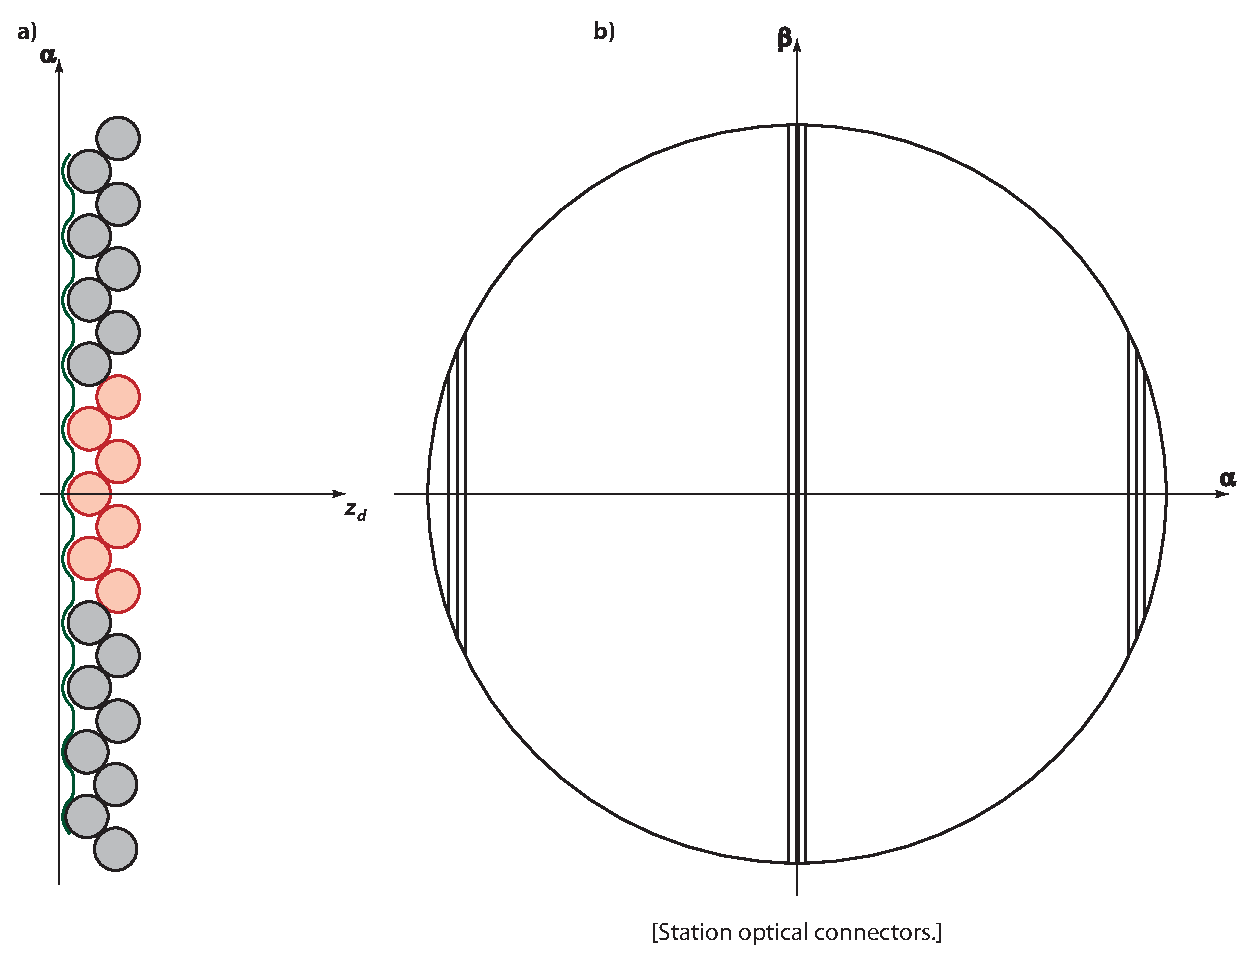
\includegraphics[width=0.95\textwidth]
      {02-Definitions/Figures/doublet-layer.eps}
  }
  \caption{
    (a) Arrangement of the doublet layers in the scintillating-fibre
    stations.  
    The outer circle shows the solenoid bore while the inner circle
    shows the limit of the active area of the tracker.  
    The grey, blue, and green regions indicate the direction that the
    individual 350\,$\mu$m fibres run (moving outward from the centre) in
    the $u$, $v$, and $w$ planes respectively.  
    (b) Detail of the arrangement of the scintillating fibres in a
    doublet layer.  
    The fibre spacing and the fibre pitch are indicated on the
    right-hand end of the figure in \,$\mu$m.
    The pattern of seven fibres ganged for readout in a single
    clear-fibre light-guide is shown in red.
    The sheet of Mylar glued to the doublet layer is indicated.
  }
  \label{Fig:DblLyr}
\end{figure}

\subsubsection{Doublet-layer numbering}
\label{SubSubSect:DblNmbrng}

The order in which the doublet layers were glued onto the station body
is shown in figure \ref{Fig:DblLyrOrder}.
The $u$ layer was glued to the station body first.
The doublet layer was glued such that the ``fibre side'' of the
doublet layer was glued to the station body; i.e. the mylar sheet
faces away from the station body.
The $w$ layer was then glued onto the outer surface of the $u$ layer.
The fibre side of the $w$ layer was glued to the mylar sheet of the
$u$ layer such that the mylar sheet of the ``w'' layer also faces away
from the station body.
Finally, the $v$ layer was glued onto the assembly.
The gluing arrangement was the same as for the $u$ and $w$ layers,
i.e. the mylar sheet of the $v$ layer also faces away from the station
body.
The numbering of the layers, which follows the order in which
the layers were glued onto the station body, is summarised in table
\ref{Tab:DblLyrOrder}.
\begin{figure}
  \begin{center}
    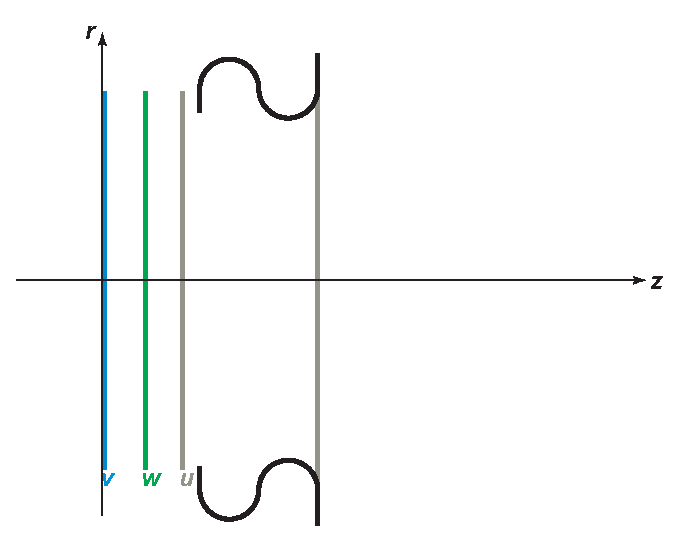
\includegraphics[width=0.55\linewidth]
      {02-Definitions/Figures/doublet-layer-order.eps}
  \end{center}
  \caption{
    The order in which the doublet layers were glued onto the station
    body. 
    The station body is indicated by the solid black lines.
    The $u$ layer (shown as the grey line) was glued to the station
    body first.
    The $w$ (indicated by the green line) was then glued onto the
    outer surface of the $u$ layer.
    The outer doublet layer, the $v$ layer (shown as the blue line)
    was then glued onto the assembly.
    The station reference surface and the direction of increasing $z$
    are shown as the thin black lines. 
  }
  \label{Fig:DblLyrOrder}
\end{figure}
\begin{table}
  \caption{
    Doublet-layer numbering scheme.
    The doublet-layer ``number'' runs from 0 to 2.
    The correspondance between the doublet layer number and the
    view is reported in the column labelled ``Doublet-layer number''.
  }
  \label{Tab:DblLyrOrder}
  \begin{tabular}{|l|r|}
    \hline
    {\bf View} & {\bf Double-layer number} \\
    \hline
    $u$        &                         0 \\
    $w$        &                         1 \\
    $v$        &                         2 \\
    \hline
  \end{tabular}
\end{table}

\subsection{Fibre-channel numbering}
\label{SubSect:FbrNmbrng}

The numbering of the groups of seven fibres ganged for readout is
shown in figure \ref{Fig:FbrChnlNmbrng}.
With the mylar surface facing up, and with the tails leading out to
the station connectors taken to be at the bottom of the figure, the
fibre-channel increases from left to right.
The coordinate measured by the doublet layer ($u$, $v$ or $w$) is
taken to increase in the same direction as the channel number.
The origin of the measured coordinate is taken to be at the position
of the central fibre.
\begin{figure}
  \begin{center}
    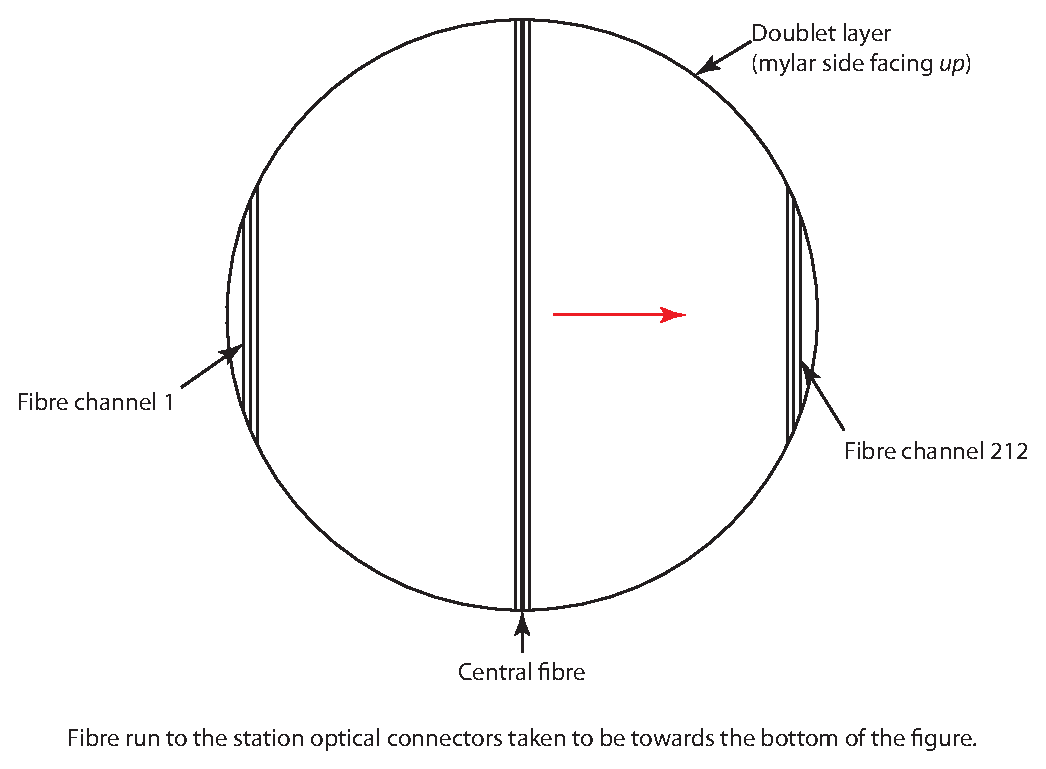
\includegraphics[width=0.75\linewidth]
      {02-Definitions/Figures/fibre-channel-numbering.eps}
  \end{center}
  \caption{
    The order in which fibre channels (groups of seven fibres) are 
    numbered.
    The senstive surface of the doublet layer is indicated by the
    solid circle.
    The direction in which the fibres run is indicated by the vertical
    lines. 
    The station optical connectors are taken to be at the bottom of
    the figure as indicated.
    With the mylar sheet taken to be facing up, fibre-channel number 1
    is to the left of the central fibre.
    The fibre-channel number increases from left to right.
    The ``zero'' of the coordinate ($u$, $v$ or $w$ increases)
    measured by the doublet layer is taken to be the position of the
    central fibre.
    The direction in which the coordinate measured by the double 
    layer increases is indicated by the red arrow. 
  }
  \label{Fig:FbrChnlNmbrng}
\end{figure}

% \section{Reference surfaces and coordinate systems}
\label{Sect:RefSurf&CoordSysts}

\subsection{Doublet layer}
\label{SubSect:RefCoordDoublet}

The doublet-layer reference surface is defined to be the flat plane that is tangential to the outer surface of the mylar plane as shown in Figure \ref{Fig:DblLyrRef&Coord}a. The measured coordinate, $\alpha \in {u, v, w}$, is defined to lie in this plane and the $\alpha$ axis is perpendicular to the direction in which the fibres run. The doublet-layer $z_d$ axis is defined to to be perpendicular to the doublet-layer reference surface increasing in the direction indicated in the figure. The direction in which the measured coordinate, $\alpha$ increases is indicated in figure \ref{Fig:DblLyrRef&Coord}b. The orthogonal coordinate in the doublet-layer reference surface that with $\alpha$ and $z_d$ completes a right handed coordinate system is referred to as $\beta$. The $\beta$ axis is also indicated in figure \ref{Fig:DblLyrRef&Coord}b.

\begin{figure}
  \begin{center}
    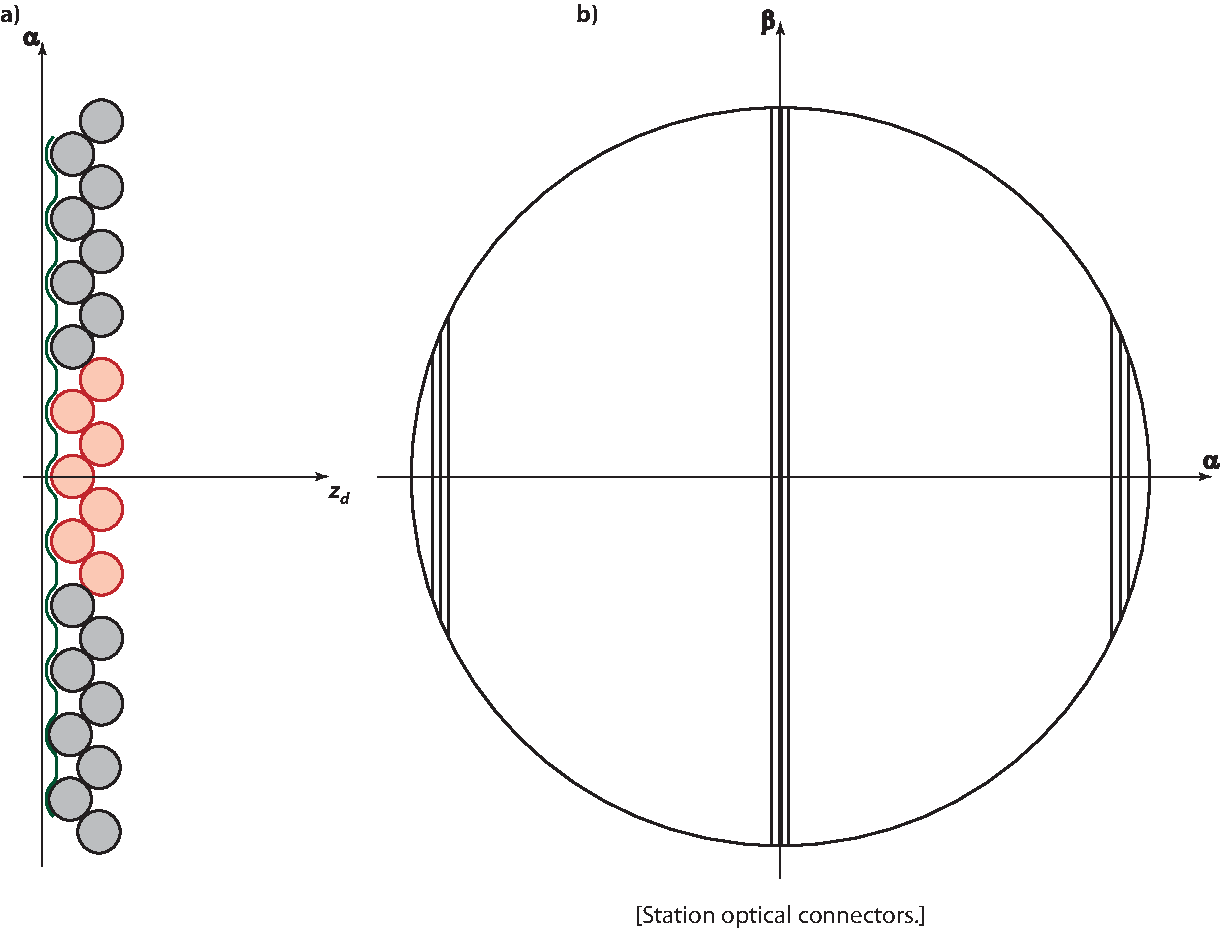
\includegraphics[width=0.7\linewidth] {detectors/tracker/03-Reference-surfaces-and-coordinate-systems/Figures/doublet-layer.pdf}
  \end{center}
  \caption{ Reference surfaces and coordinate-system definitions for the double layer and station. a) The fibres in the doublet layer are shown as the shaded circles, the central channel being shaded pink. The mylar layer is indicated by the solid black corrugated line. The doublet-layer reference surface is indicated by the vertical straight line, the arrow labelled $\alpha$ indicates the direction in which the coordinate measured by the doublet layer ($u$, $v$ or $w$) increases. The direction of the $z_d$ axis is indicated. b) View of doublet layer looking down on the mylar layer with the optical connectors at the bottom of the figure. The coordinate measured by the doublet layer ($u$, $v$ or $w$) is indicated by the axis labelled $\alpha$. The orthogonal axis, i.e. the direction in which the fibres run, is labelled $\beta$. The origin of the $(\alpha, \beta)$ coordinate system is taken to be at the centre of the circular active area.}
  \label{Fig:DblLyrRef&Coord}
\end{figure}

\subsection{Station}
\label{SubSect:RefCoordStn}

The station reference surface is defined to coincide with the reference surface of the $v$ doublet layer (see figure \ref{Fig:StnRef&Coord}). The station coordinate system is defined such that the $y_s$ axis is coincident with $v$ axis, the $z_s$ axis is coincident with the $z_d$ axis of the $v$ layer and the $x_s$ axis completes a right-handed coordinate system.

\begin{figure}
  \begin{center}
    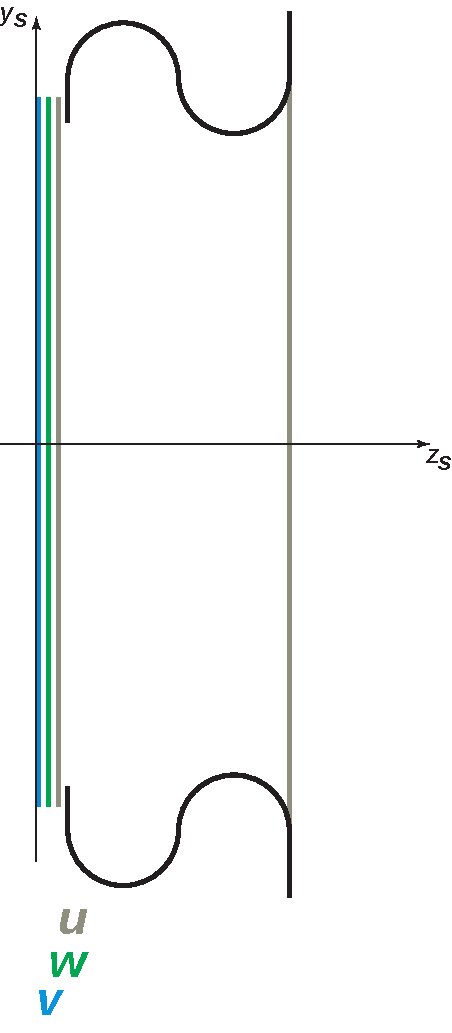
\includegraphics[width=0.22\linewidth]{detectors/tracker/03-Reference-surfaces-and-coordinate-systems/Figures/station.pdf}
  \end{center}
  \caption{ The carbon-fibre station body is indicated by the heavy solid black lines. The three doublet layers are indicated by the solid grey ($u$), green ($w$) and blue ($v$) lines. The station reference surface is shown by the solid vertical line coincident with the reference surface of the doublet layer labelled $v$. The direction $y_s$ axis, defined to be coincident with the $v$ axis and the $z_s$ axes are shown as the solid, black arrows. The $x_s$ axis completes a right-handed coordinate system and therefore points into the page. }
  \label{Fig:StnRef&Coord}
\end{figure}

\subsection{Tracker}
\label{SubSect:TrkrCoordStn}

The tracker reference surface is defined to coincide with the reference surface of station 1. The tracker coordinate system is defined such that the $z_t$ axis coincides with the nominal axis of cylindrical symmetry of the tracker as shown in figure \ref{Fig:TrkRef&Coord}. The tracker $z_t$ coordinate increases from station 1 to station 5. The tracker $y_t$ axis is defined to coincide with the $y_s$ axis of station 1 and the tracker $x_t$ axis completes a right-handed coordinate system.

\begin{figure}
  \begin{center}
    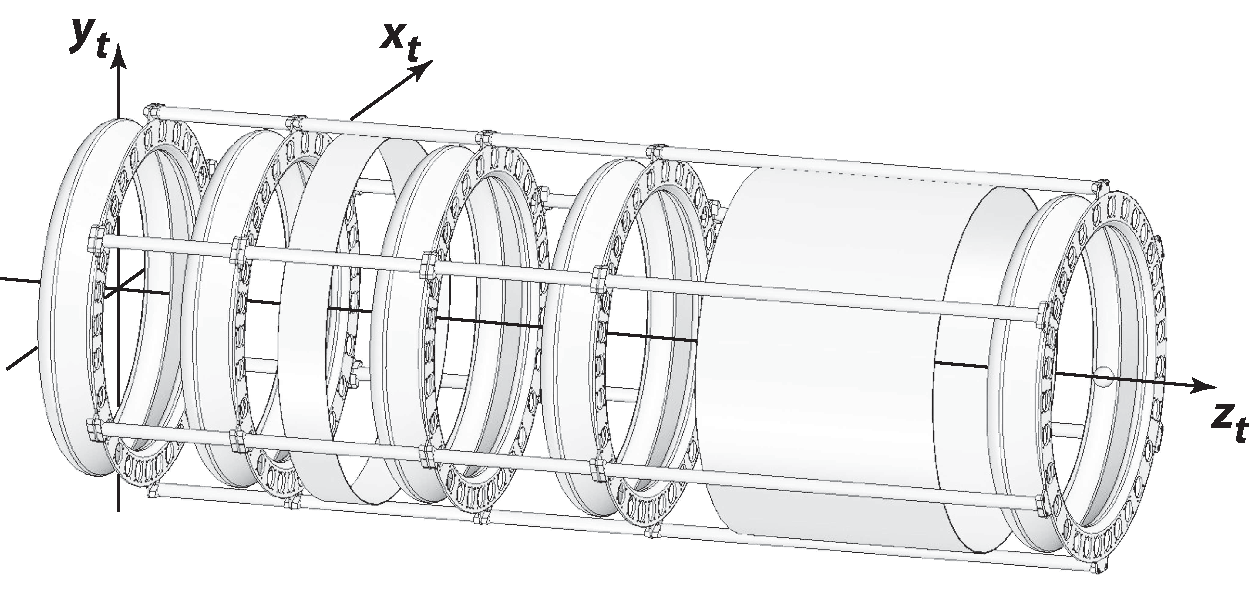
\includegraphics[width=0.7\linewidth]{detectors/tracker/03-Reference-surfaces-and-coordinate-systems/Figures/tracker.pdf}
  \end{center}
  \caption{ The outline of the components that make up the MICE tracker are shown in the line drawing. The tracker reference surface coincides with the reference surface of station 1. The tracker coordinate system is indicated by the solid lines. The $y_t$ axis is defined to be coincident with the $y_s$ axis in the station coordinate system.  The $z_t$ axis runs along the nominar axis of the tracker. The $x_t$ axis completes a right-handed coordinate system. }
  \label{Fig:TrkRef&Coord}
\end{figure}

\subsection{Coordinate transformations}
\label{SubSect:CoordTran}

\subsubsection{Doublet-layer to station}
\label{SubSubSect:DblStn}

The transformation from doublet-layer to station coordinates is achieved using the rotation $\underline{\underline{R}}_{SD}$ defined by: 

\begin{equation}
  {\bf r_s} = 
    \left(
        \begin{array}{c}
           x_s                                                      \\
           y_s
        \end{array}
    \right) = \underline{\underline{R}}_{SD} {\bf m} =
    \left(
        \begin{array}{cc}
           \cos \theta_D & -\sin \theta_D                           \\
           \sin \theta_D & -\cos \theta_D
        \end{array}
    \right) 
    \left(
        \begin{array}{c}
           \alpha                                                   \\
           \beta
        \end{array}
    \right) \, ;
\end{equation}
where $\theta_D$ is the angle which the fibres that make up the doublet-layer make to the $x_s$ axis in the station coordinate system.

% \section{Reconstruction}
\label{Sect:Recons}

\input 04-Reconstruction/04-01-Hits-and-clusters/04-01-Hits-and-clusters
\input 04-Reconstruction/04-02-Space-points/04-02-Space-points
\input 04-Reconstruction/04-03-Pattern-recognition/04-03-Pattern-recognition
\input 04-Reconstruction/04-04-Track-fit/04-04-Track-fit

% \section{Data structure}
\label{Sect:DataStructure}

{\bf Lead author:} Adam

% \section{Algorithms}
\label{Sect:Algor}

{\bf Lead author:} Adam

% \section{Configuration data base}
\label{Sect:ConfigDB}

{\bf Lead author:} Adam

% \section{The Monte Carlo}
\label{Sect:SciFiMonteCarlo}

The tracker Monte Carlo can be run using the script at the beginning of the tracker section.  In addition to the basic Monte Carlo noise from dark count in the VLPCs can be simulated by including the mapper MapCppTrackerMCNoise, which should be run before MapCppTrackerMCDigitization.  Reconstruction after digitization is agnostic to source by design decision.

\subsection{Station Geometry}
The tracker geometry is built in Geant4 on a fibre-by-fibre basis.  The size of the active tracker plane and the fibre diameter is defined in the mice modules.  The fibre offset and translation are determined in code, the length of the fibres are then determined by its position within the plane.  Fibre placement is then iterated over from one end of the plane to the other filling in all gaps within the area.

Each of the three scintillating fibre planes is built up this way.  In addition to these the Monte Carlo also includes a thin layer of mylar sandwiched between these planes.  The relative position of the three tracking planes and the three mylar layers within the station are defined in the mice modules.

\subsection{MC VLPC Dark Count}
When the mapper MapCppTrackerMCNoise is included in the MC each channel is tested for the presence of an integer number of PE randomly appearing in the data.  The chance of this per channel noise is defined by the parameter SciFiDarkCountProbabilty within the data cards, while the number of PE generated is given by a Poisson distribution.  If a noise hit is produced it is recorded to be passed to digitization later. 

\subsection{Building Digits}
When a particle crosses a scintillating fibre in the MC it may deposits some amount of energy in passing determined by Geant4.  The digitization process takes this deposited energy and transforms it into a number of PE as follows: 

\begin{multline}
NPE = Energy \times SciFiFiberConvFactor \times SciFiFiberTrappingEff \times \\
      ( 1.0 + SciFiFiberMirrorEff ) \times SciFiFiberTransmissionEff \times \\
      SciFiMUXTransmissionEff * SciFivlpcQE;
\end{multline}

\noindent
Where the value of each of these variable other than the deposited energy is given in the data cards.

Hits in the same tracker, station, and plane are collected together to form a single digit.  The grouping of digits are merged with any noise effects and a Gaussian smearing is applied to the total NPE to finish the digitization process.

% \section{Performance}
\label{Sect:Performance}

{\bf Lead author:} Adam, Ed and Chris

%\include{detectors/emr}
%\include{detectors/ckov}
%\include{detectors/kl}

\chapter{The Envelope Tool}

The MAUS envelope tool is intended as a tool to support lattice development and
enable visualisation of the MICE accelerator for online use. The tool 
facilitates the visualisation of field elements, propagation of particles and
beams ellipses through those elements.

The envelope tool is intended for use with mostly straight beamlines.

\section{Example Usage}
To call the envelope tool with some example data, source the MAUS environment 
and then do

\begin{verbatim}
$ python ${MAUS_ROOT_DIR}/bin/utilities/envelope_tool/envelope_tool.py \
  --configuration_file ${MAUS_ROOT_DIR/}bin/utilities/envelope_tool/share/pseudobeamline.py
\end{verbatim}

\begin{figure}[!htb]
\centering
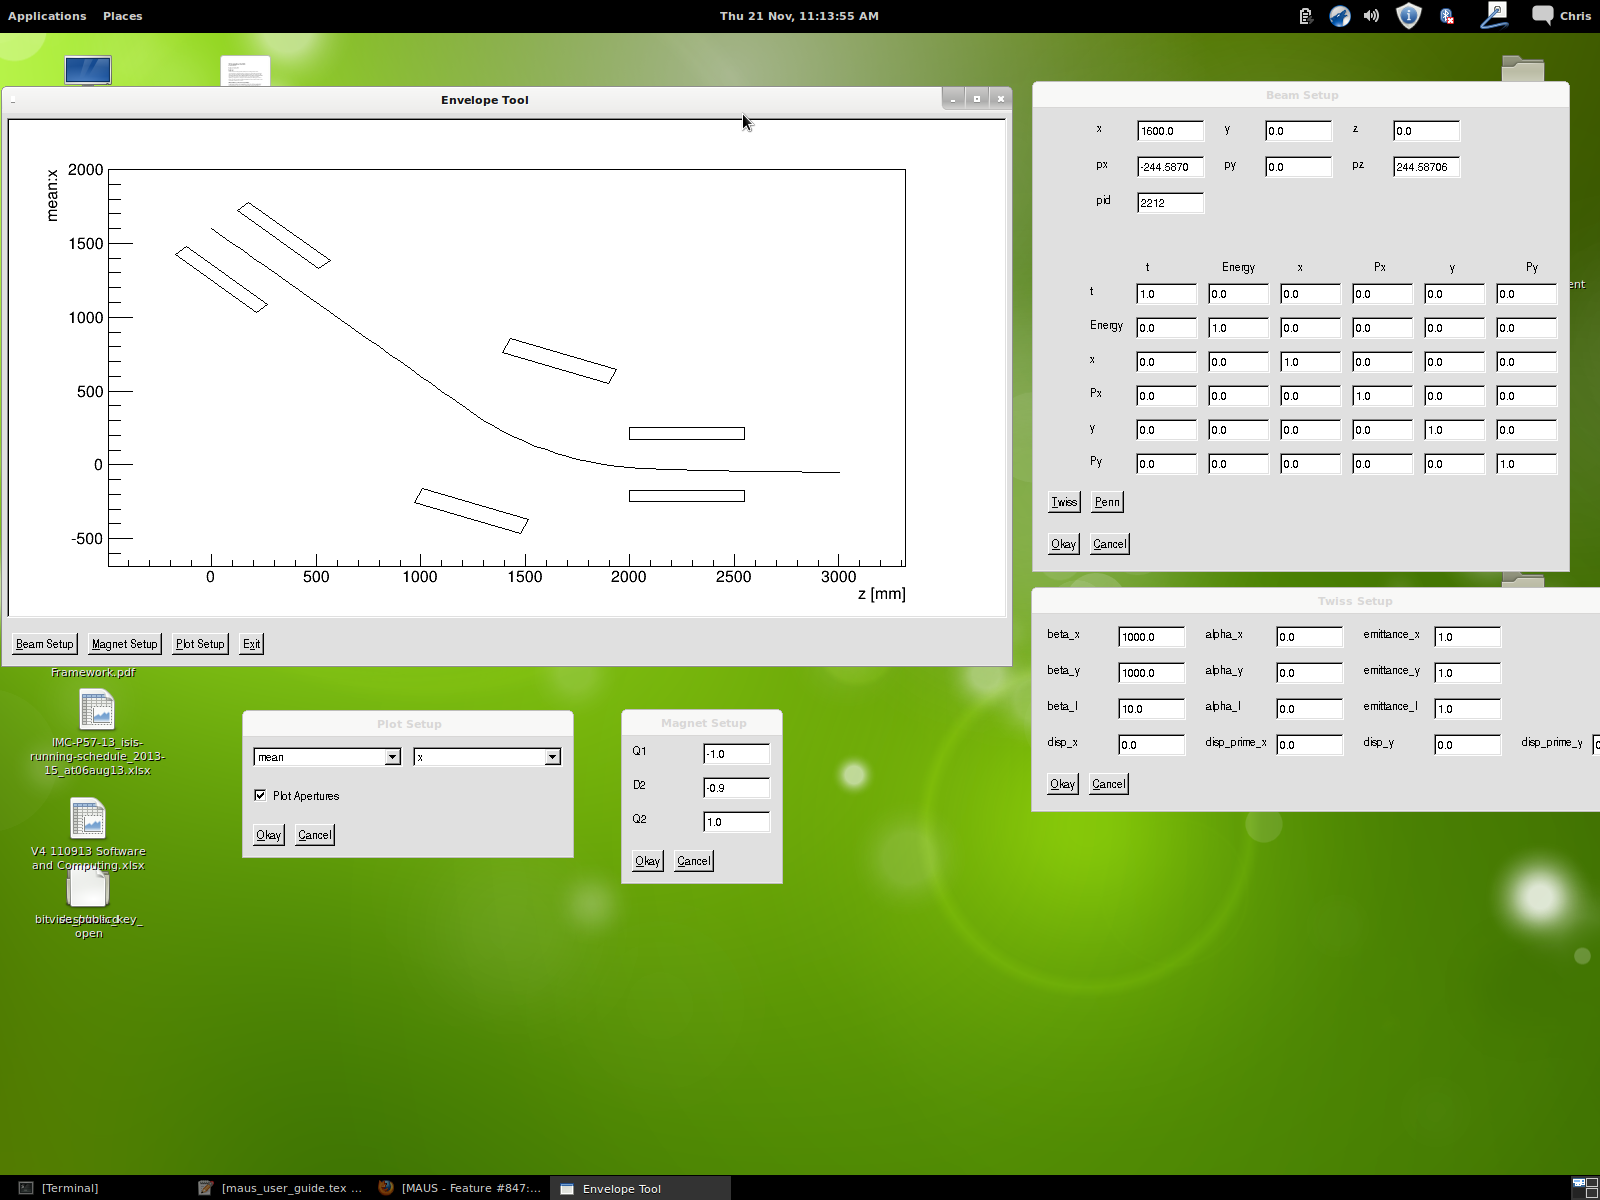
\includegraphics[width=0.9\textwidth]{envelope_tool.png}
\caption{The Envelope Tool used to plot a reference trajectory through a few magnets.}
\end{figure}

\section{Envelope Tool main window}
The Main Window enables the user to view the selected lattice parameters, and
provides buttons to update the beam, lattice and plot parameters.

\begin{itemize}
\item Beam Setup: setup a beam
\item Magnet Setup: setup fields
\item Plot Setup: setup the plot
\item Exit: exit the GUI
\end{itemize}

\section{Beam Setup}

The Beam Setup window enables the user to set beam parameters. The top few cells
set initial position, momentum and particle type of the beam centroid, also
referred to as the `reference particle' or `reference trajectory'. The bottom
few cells set beam ellipse parameters.

Helper windows can be accessed to parameterise the beam ellipse using either a
Penn parameterisation or a
Twiss parameterisation.

\begin{itemize}
\item x, y, z: initial position of the beam particle
\item px, py, pz: initial momentum of the beam particle
\item pid: PDG ID of the beam particle. This is an integer; see Tab. 
\ref{tab:pdg_id} for some common particle ids.
\item ellipse elements: set the elements of the beam ellipse.The matrix must
be symmetric and positive definite or an error will be returned when Okay is
pressed.
\item Twiss: setup the beam using a Twiss parameterisation - beam asymmetric in
x and y with no coupling
\item Penn: setup the beam using a Penn parameterisation - beam cylindrically 
symmetric in x and y with angular momentum
\item Okay: click okay to return to the main window, updating the beam ellipse
\item Cancel: click cancel to return to the main window, losing changes
\end{itemize}

\section{Magnet Setup}
The user can manipulate magnet parameters in this window. When the window is
opened, MiceModules which have the following required parameters are added to
the window.

\begin{itemize}
\item FieldType (string)
\item FieldName (string)
\item Position (hep three vector)
\item Rotation (hep three vector)
\item ScaleFactor (double)
\item NominalAperture (hep three vector)
\item NominalOuter (hep three vector)
\end{itemize}

Other MiceModules will be ignored.

Each magnet is labelled with the magnet FieldName and a text entry is available
to set the scale factor (proportional to field).

\begin{itemize}
\item <field entries>: Enter a float to set the scale factor.
\item Okay: Update the fields in the lattice
\item Cancel: Cancel changes
\end{itemize}

\section{Plot Setup}
The Plot Setup window enables the user to select the desired plot parameters.

\begin{itemize}
\item Plot Type: Select the type of variable to plot.
\item Plot Variable: Select the variable to plot.
\item Plot Apertures: tick to plot physical apertures. If the plot type is
\verb|mean| or \verb|envelope| and plot variable is \verb|x| or \verb|y| the 
apertures will be 
plotted as a 2D projection of the physical apertures in the appropriate plane,
with the beam reference trajectory or beam envelope superimposed. Note that the
rotations applied here are rather simplistic, assuming a 2D geometry in x or y
plane (but not both) Otherwise nominal apertures will be scaled to fit in the 
upper portion of the plotting window.
\item Okay: Update the plot in the main window with the new selection.
\item Cancel: Cancel changes
\end{itemize}


 % envelope utility - could be an appendix


%\chapter{Geometry}
%\include{geometry_definitions}

%\chapter{Appendix A: Run Control Variables}
%\include{run_controls} % automatically constructed by build script

%\chapter{Appendix B: Spill Structure}
%\include{spill_schema} % automatically constructed by build script
%

\end{document}

